% buaa基于ctexbook模板
% 模板选项:
%======================
% I.论文类型(thesis)
%--------------------
% a.学术硕士论文(master)[缺省值]
% b.专业硕士论文(professional)
% c.博士论文(doctor)
%--------------------
% II.密级(permission)
%--------------------
% a.公开(public)[缺省值]
% b.内部(privacy)
% c.秘密(secret=secret3)
% c.1.秘密3年(secret3)
% c.2.秘密5年(secret5)
% c.3.秘密10年(secret10)
% c.4.秘密永久(secret*)
% d.机密(classified=classified5)
% d.1.机密3年(classified3)
% d.2.机密5年(classified5)
% d.3.机密10年(classified10)
% d.4.机密永久(classified*)
% e.绝密(topsecret=topsecret10)
% e.1.绝密3年(topsecret3)
% e.2.绝密5年(topsecret5)
% e.3.绝密10年(topsecret10)
% e.4.绝密永久(topsecret*)
%--------------------
% III.打印设置(printtype)
%--------------------
% a.单面打印(oneside)[缺省值]
% b.双面打印(twoside)
%--------------------
% IV.系统类型(ostype)
%--------------------
% a.win(oneside)[缺省值]
% b.linux (linux)
% c.mac (mac)
%--------------------
% V.ctexbook设置选项(<ctexbookoptions>)
%--------------------
% ...
%======================
% 其他说明:
% 1. Mac系统请使用mac选项,并使用XeLaTeX编译。
% 2. 可加入额外ctexbook文档类的选项,其将会被传递给ctexbook。
%    例如:\documentclass[fontset=founder]{buaa}
% 3. CTeX在Linux下默认使用Fandol字体,为避免某些生僻字无法显示,在系统已安装方正
%    字体的前提下可通过fontset=founder选项常用方正字体。
%=================================================================
% buaa模板已内嵌以下LaTeX工具包:
%--------------------
% ifthen, etoolbox, titletoc, remreset,
% geometry, fancyhdr, setspace,
% float, graphicx, subfigure, epstopdf,
% array, enumitem,
% booktabs, longtable, multirow, caption,
% listings, algorithm2e, amsmath, amsthm,
% hyperref, pifont, color, soul,
% ---
% For Win: times
% For Lin: newtxtext, newtxmath
% For Mac: times, fontspec
%--------------------
% 请在此处添加额外工具包>>
%=================================================================
% buaa模板已内嵌以下LaTeX宏:
%--------------------
% \highlight{text} % 黄色高亮
%--------------------
% 请在此处添加自定义宏>>
%%=================================================================

%master代表学硕 professional代表专硕,其他默认就好
\documentclass[master,public,twoside,win,AutoFakeBold]{buaa}


%============================== 格式设置 ===================================
% 开启/关闭引用编号颜色:参考文献,公式,图,表,算法 等……
\refcolor{off}   % 开启: on; 关闭: off[默认];

% 双面打印时增加·空白页·保证封面、目录、摘要和每章的起始页在奇数页。
% 最终论文可以单面打印,一般不需要打开。
\beginright{off} % 开启: on; 关闭: off[默认];
% 上个命令增加的空白页,设置内容
\emptypagewords{[ -- This page is a preset empty page -- ]}

%盲评模式,开启后不显示学校等信息 ,注意注释致谢部分。
\blindmode{off}  % 开启: on; 关闭: off[默认];

%首页是否改为蓝色封皮,论文提交图书馆保证首页为蓝色封皮。
\bluecover{on}  % 开启: on; 关闭: off[默认];

% 图表目录 ---% 启用: on[默认]; 关闭: off;
\Listfigtab{on} 




%============================= 内容填写 ====================================
% 论文题目-{中文}{英文}
\Title{基于可微分渲染的三维重建与纹理优化}{3D Reconstruction and Texture Optimization based on Differentiable Rendering}

%论文副标题-{中文}{英文},没有副标题注释即可。
% \Subtitle{}{}

% 学位级别
\Branch{工学硕士}

% 院系,专业及研究方向
\Department{计算机科学与技术学院}

% 一级学科/学科专业 
\Major{计算机科学与技术} % 学硕写`计算机科学与技术` 专硕写 `电子信息`

% 二级学科 
\Majorsec{计算机科学与技术} % 学硕写`计算机科学与技术` 专硕写 `软件工程`

%研究方向
\Field{纹理优化}

% 第一导师信息 
\Tutor{赵海峰}{Zhao Haifeng}{教授} % {中文名}{英文名}{职称}

% 第二导师信息,如果没有第二导师,注释下面一行即可。
\Cotutor{付燕平}{Fu Yanping}{讲师} % {中文名}{英文名}{职称}

% 学生姓名 
\Author{刘勇鑫}{Liu Yongxin} % {中文名}{英文名}

% 中图分类号,不用填写
\CLC{}

% 论文编号 ---10357+自己学号
\StudentID{10357E20201107}

% 时间节点 
%入学时间
\DateEnroll{09}{01}{2020} % {月}{日}{年}

%毕业时间
\DateGraduate{07}{01}{2023} % {月}{日}{年}

%论文提交日期
\DateSubmit{05}{23}{2023} % {月}{日}{年}

%论文答辩日期
\DateDefence{05}{15}{2023} % {月}{日}{年}


%%=================================================================
% 摘要 ---{中文}{英文}
\Abstract{%
    三维重建是VR/AR、动画游戏等领域的重要应用之一,需要实现高保真的纹理映射和精细的几何重建。然而,由于现有的基于RGB-D相机的三维重建算法不可避免的遭受噪音的影响,会出现重建模型几何细节丢失和扭曲的问题导致几何误差。在重建的过程中,每一帧的相机位姿依赖于前一帧的计算结果,在计算过程中误差不可避免。经过时间的推移误差会随之累积,估计的相机位姿就会偏离真实位置,从而出现相机位姿估计误差。 受上述误差的影响,在纹理映射过程中,模型顶点投影至图像平面上时就会偏离正确投影位置。通过颜色加权融合后得到的纹理会出现模糊和重影等瑕疵。针对几何误差和相机位姿误差对纹理映射结果的影响,本文提出了两个有效的算法分别对他们造成的纹理映射模糊和重影等纹理进行优化,从而得到高质量、高保真的纹理模型。\par
    为了解决相机位姿估计误差对纹理带来的影响,本文基于可微分渲染提出了一个端到端的优化方法,对相机姿态和纹理进行改进。首先,使用光度一致性纠正几何模型顶点到每个视角的映射关系,然后利用对抗神经网络学习误差容忍度量,容忍纹理重建过程中存在的各种误差。本文方法经过实验证明能够消除初始纹理存在的缺陷,如模糊、伪影和裂缝等。相比于传统方法,本文方法适用于各种具有挑战性的场景,并且可以弥补传统方法泛化能力不足的缺陷。\par
    虽然矫正相机位姿与纹理重合成算法可以降低纹理映射中的位姿误差和噪声影响,但是当重建模型存在严重错位或几何细节缺失时,难以达到理想效果。因此,针对几何误差带来的影响。本文提出了基于可微分渲染的几何矫正方法,它能够通过更新几何模型的顶点位置来重建模型的表面形状。此外,本文采用基于三角形质心的自适应细分方法,以增加几何模型表面的平滑度,从而更容易恢复高频几何细节。最后,本文基于可微分渲染提出了一个联合优化深度学习框架,对相机位姿、纹理和几何模型进行联合优化。这种联合优化方式能够克服单独优化某一因素难以达到全局最优解的限制,从而得到高质量的重建模型。实验结果表明,在公共数据集上,本文提出的联合优化框架相比于其他最新纹理优化方法,在恢复三维重建模型高质量几何细节和高保真纹理细节方面表现更好。
}
{%

    3D reconstruction is one of the important applications in VR/AR, animation and gaming industries, requiring high-fidelity texture mapping and fine geometric reconstruction. However, as the existing 3D reconstruction algorithms based on RGB-D cameras inevitably suffer from noise, the problem of loss of geometric details and distortion of the reconstructed model can lead to geometric errors. In the reconstruction process, the camera pose of each frame depends on the calculation result of the previous frame, and the error is inevitable during the calculation process. The errors will accumulate over time and the estimated camera pose will deviate from the true position, resulting in camera pose estimation errors. As a result of the above errors, the model vertices will deviate from the correct projection position when they are projected onto the image plane in the texture mapping process. The textures obtained by color-weighted fusion will have defects such as blurring and ghosting. To address the effects of geometric errors and camera positional errors on texture mapping results, two effective algorithms are proposed in this thesis to optimize textures such as blurring and ghosting caused by them, respectively, so as to obtain high-quality and high-fidelity texture models.\par
    
     To address the impact of camera pose estimation errors on texture,this thesis proposes an end-to-end optimization method based on differentiable rendering to improve camera poses and textures, addressing the impact of camera pose estimation errors on texture. Firstly, the mapping relationship between the geometry model vertices and each viewpoint is corrected using photometric consistency. Then, an adversarial neural network is employed to learn an error-tolerant metric, accommodating various errors that may exist during the texture reconstruction process. Experimental results demonstrate that this method effectively eliminates the defects present in the initial texture, such as blurring, ghosting, and seams. Compared to traditional methods, this approach is applicable to various challenging scenarios and can compensate for the limitations of traditional methods in terms of generalization capabilities.\par
    
    While the camera pose alignment and texture compositing algorithms can mitigate the effects of pose estimation errors and noise in texture mapping, they face difficulties in achieving satisfactory results when there are severe misalignments or geometric details missing in the reconstructed models. Therefore, to tackle the impact of geometric errors, this thesis proposes a differentiable rendering-based geometry correction method that updates the vertex positions of the geometry model to reconstruct the surface shape. Additionally, an adaptive subdivision method based on triangle centroids is employed to increase the smoothness of the geometry model surface, facilitating the recovery of high-frequency geometric details. Finally, a joint optimization deep learning framework based on differentiable rendering is proposed to optimize camera poses, textures, and geometry models collectively. This joint optimization approach overcomes the limitations of separately optimizing individual factors, enabling the generation of high-quality reconstructed models. Experimental results on public datasets demonstrate that the proposed joint optimization framework outperforms other state-of-the-art texture optimization methods in recovering high-quality geometric details and high-fidelity texture details in 3D reconstruction models.\par
}
\vspace{-5em}

% 关键字 ---{中文}{英文}
\Keyword{%
三维重建,纹理优化,几何模型优化,相机位姿矫正,可微分渲染
}{%
3D reconstruction, texture optimization, geometry model optimization, camera pose correction, differentiable rendering
}


\begin{document}

%%=================================================================
% 标题级别
%--------------------
% \chapter{第一章}
% \section{1.1 小节}
% \subsection{1.1.1 条}
% \subsubsection{1.1.1.1}
% \paragraph{1.1.1.1.1}
% \subparagraph{1.1.1.1.1.1}
%--------------------
%%=================================================================


% 第一章绪论
% !TeX root = ../Template.tex
% [绪论]
% 此处为本LaTeX模板的简介

% \clearemptydoublepage
% \setcounter{figure}{0}
% \setcounter{table}{0}
% \setcounter{algocf}{0}
% \chapter{绪 论}

\chaptera{绪 论}


% 从应用角度来看,三维重建技术可以获取物体的准确三维信息,从而帮助人们更好地理解和分析真实世界的物体,并且可以为计算机图形学、机 
% 器人、虚拟现实等应用提供基础。例如,在计算机图形学中,三维重建技术可以用来创建或者模拟真实世界中的场景;在机器人领域,三维重建 
% 技术可以用来帮助机器人更好地感知环境;在虚拟现实领域,三维重建技术可以用来创建虚拟场景等。

计算机视觉是指利用计算机自动处理图像数据,以解决计算机像人眼一样处理图像问题的技术。三维重建是一种利用计算机视觉和图像处理技术,将真实世界中的物体或场景从二维图像或视频中还原成三维模型的技术过程。RGB-D深度相机能同时捕捉场景颜色信息和深度信息,为计算机视觉、机器人技术、虚拟现实等应用提供了硬件支持。借助于RGB-D相机,可以方便地进行三维重建和纹理重建,极大地减少重建成本,并且可以恢复出精确的三维场景结构和纹理信息。

%%============================

%缺乏图示,vr纹理应用图示,缺乏引用
\section{研究背景与意义}
从图片和视频中恢复出三维场景是计算机视觉领域中的重要研究方向,也是场景理解与分割的重要研究基础。三维重建技术有广泛的应用前景,在建筑、汽车制造、医疗、无人机、游戏、电影制作等领域都有很大的需求。例如,在建筑领域,三维重建技术可以被用于制作建筑物的三维模型,从而更便于设计和建造;而在医疗领域,可以将其用于制作身体的三维模型,帮助医生进行手术规划。在无人机领域,三维重建技术可以被用于制作地面的三维模型,从而更好地辅助无人机的导航;在电影制作领域,三维重建技术可以被用于打造电影中真实的三维场景,从而更好地让观众融入故事情境中。\par
单纯的RGB图像无法准确地恢复出场景的三维结构。由于RGB图像中的物体符合近大远小的规则,导致重叠的物体之间存在深度模糊,无法确定图像中物体的远近关系。因此,需要额外的深度信息来确定图像中物体之间的相对距离。早期的三维重建缺乏直接的深度数据可用,需要利用多个视角之间的视差关系来估计物体深度。然而,这种方法得到的深度误差较高,不仅使得重建过程时间长,而且还可能导致重建结果的不准确,重建出的模型一直无法令人满意。得益于深度相机的出现,现在可以利用该设备获取场景中光线行进路径上的物体与相机之间的距离,重建出具有精细几何细节的稠密三维场景模型。这为三维重建技术的发展提供了硬件支持。RGB-D相机能够直接获取相机光心到物体表面的距离,相比于早期的多视角视差方法,基于该相机的三维重建技术能够实时处理深度数据并在短时间内重建出高精度的场景模型。\par
虽然RGB-D深度相机可以获取相对准确的深度数据,可以提高三维重建模型的效率和准确性。但是,由于深度相机分辨率较低,拍摄图片清晰度不高,重建出模型很容易丢失微小的几何细节。不仅如此,深度相机普遍采用红外光测量距离,容易受太阳光和室内其他光源的影响,产生深度测量噪声与度量误差。并且相机本身在制造过程中可能会出现镜头变形,使得拍摄图片受到切向畸变或者径向畸变影响,导致三维模型顶点投影至平面时发生错位现象。以上深度相机固有的缺陷使得测量数据不可避免地含有噪声,造成三维重建模型的瑕疵和高频几何细节的缺失。三维重建中估计相机位姿时往往采用增量融合的方式,这种方法需要重复地将每一帧的数据与前一帧的结果进行融合,以逐步构建出全局的三维模型。由于估计误差不可避免,这种误差一直会累计并传递至下一帧,导致相机出现漂移现象。即使有回环矫正等位姿修正方法,位姿估计误差也无法完全消除,最终造成重建出的三维模型几何形状偏离预期。在三维模型纹理生成阶段,三维模型中每个顶点会投影至不同彩色图像上以获得顶点颜色。由于几何误差和相机位姿估计误差的存在,同一个顶点投影至不同视角关联的彩色图像时往往会出现偏移,得到不一致的颜色。加权平均后使得纹理映射出现模糊和重影现象。\par
由于存在以上误差,纹理重建结果无法让人满意,在实际应用中仍需人工进行一定的干预。要想获取清晰纹理,必须首要解决相机位姿估计不准确的问题。然后,解决由于几何误差而导致纹理不能和几何模型对齐的瑕疵。先前的工作在提升纹理映射质量方面做出了许多努力。一些方法致力于提升重建模型质量,间接提高纹理映射结果。另外一些方法采用扭曲彩色图像的方法弥补相机位姿的误差。还有一些方法采用联合优化方法,同时矫正相机位姿、恢复三维重建模型几何细节和估计场景光源,来共同提升几何和纹理质量。受可微分渲染方法在单视图三维重建领域\upcite{ShichenLiu2019SoftRA}获得成功的影响,本文采用可微分渲染方法矫正相机位姿,将可微分渲染模块嵌入对抗神经网络中,合成近似真实场景外观的纹理图像。进一步,本文基于可微分渲染提出联合优化框架,不仅能提升纹理质量而且能恢复几何模型的高频细节,得到高保真的纹理。\par
综上所述,本文提出了利用可微渲染矫正相机位姿和采用对抗神经网络合成纹理的策略,以解决纹理映射中存在的模糊和伪影问题。此外,本文在第一个纹理优化框架的基础上,提出了一种联合优化方法,不仅可以提升几何模型重建质量,还可优化纹理以弥补纹理与几何模型存在的错位现象,获得更高保真的纹理模型。
%%============================
\section{研究现状}
\subsection{三维重建}
虽然三维重建技术非常复杂,但随着视觉传感器的进步,不断涌现出各种三维重建算法。其中,基于RGB-D相机的三维重建技术源自于同时定位和地图构建(Simultaneous Localization and Mapping,SLAM)。这是计算机视觉中的一项重要技术,可以通过观察周围环境,确定机器人的位置并重建场景地图。SLAM 涉及多个不同的领域和技术,因此它具有多个分支和分类方法。根据使用的传感器类型不同,SLAM 技术可以分为多类,如视觉SLAM、激光SLAM、惯性SLAM和深度SLAM等。其中,视觉SLAM 利用摄像头或 RGB-D 相机等视觉传感器获取环境图像信息,并通过计算机视觉算法进行处理和分析,能够在未知环境下,对机器人位置和姿态进行估计,并构建地图。在本文中,为了方便起见,将 RGB-D 相机出现之前的视觉 SLAM 技术统称为传统 SLAM。与传统 SLAM 不同,基于 RGB-D 相机的三维重建不仅采用彩色信息,还利用深度信息,并以深度信息为主。传统 SLAM 主要依赖彩色图像信息,其主要目标是定位,次要目标是建图,而且它只能构建稀疏图。基于 RGB-D 相机的三维重建以建图为主体,可以构建稠密高质量的地图,以满足实际应用需求。从 KinectFusion\upcite{RichardNewcombe2011KinectFusionRD} 开始,利用 RGB-D 相机实时重建完整且精密的地图,引发了以 RGB-D 相机作为传感器的 SLAM 技术热潮。后续大部分重建算法为了保持一致,算法名称中均带有单词 “Fusion”,因此基于 RGB-D 相机的三维重建和基于 Fusion 的三维重建是等价的。基于 RGB-D 相机的三维重建可以进一步细分为静态场景的重建和动态场景的重建,但是本文研究的纹理优化是基于静态场景的,因此接下来只介绍静态场景相关的工作。\par

2011年,以KinectFusion为代表的三维重建算法问世,它使用Kinect传感器采集的深度数据,实时融入到截断符号距离场(Truncated Signed Distance Function,TSDF)模型表示中。TSDF是一种三维重建技术,通过将物体所在的空间分割成多个小的立方体块来构建三维实体。每个立方体块的数值表示该块与其最近的物体表面之间的距离。KinectFusion使用帧到模型的最近邻迭代算法(Iterative Closest Points Algorithm,ICP),根据当前帧与全局模型的对应关系,获得每帧图像的相机位姿变换。由于采用稠密体积表示,内存开销大,并且易受相机位姿估计误差影响,因此很难重建大型场景的三维模型。Thomas Whelan等人\upcite{ThomasWhelan2012KintinuousSE}提出了更完备的三维重建系统Kintinuous。相较于KinectFusion,Kintinuous融合了回环检测和回环矫正,以避免位姿估计误差积累导致相机跟踪失败。此外,它使用变形图进行非刚性变换,通过更新模型顶点的空间坐标,减少误差积累,更适合大场景的三维重建。
进一步地,Thomas Whelan等人\upcite{ThomasWhelan2015ElasticFusionDS}提出了采用面元素(Surfel)而非体素的模型表示方法的ElasticFusion。它可以实时捕获稠密的表面地图,并且能够检测多个光源的位置,提高地图质量、跟踪精度和鲁棒性。但是,它需要较高的内存和计算资源,更适合小场景的重建。Prisacariu等人\upcite{VictorAdrianPrisacariu2017InfiniTAMVA}提出了InfiniTAM v3,用于在大范围场景中进行深度信息融合和跟踪的跨平台实时跟踪框架。它采用哈希表来存储隐式体积表示,能够重建比KinectFusion更大范围的3D环境。Angela Dai等人\upcite{AngelaDai2016BundleFusionRG}提出并行化的优化框架Bundlefusion,利用光束平差法(Bundle Adjustment,BA)来优化三维重建模型中相机的位置和物体的三维坐标,以使得重建结果与观测数据之间的误差尽可能小。同时,它利用RGB-D相机采集的彩色和深度图像,通过在线表面重整和全局位姿矫正,得到全局一致的三维重建结果。

最近,神经辐射场(Neural Radiance Fields,Nerf)技术在三维重建领域迅速发展。Dejan等人\upcite{DejanAzinovic2021NeuralRS}提出了基于神经辐射场的非实时三维重建框架,利用神经网络存储符号距离场的隐式表达,得到比单独使用基于颜色或深度数据的方法更详细和完整的重建结果。\par

虽然以上的方法采用各种不同的策略抵抗了在重建过程中采集到的深度数据噪声以及估计相机位姿的累计误差,但是由于重建算法固有的缺陷,生成的三维模型仍然存在几何细节丢失和瑕疵等现象。

\subsection{纹理优化}
三维重建利用计算机技术构建真实场景,需要准确恢复场景的几何形状和表面外观,通过正确的纹理映射可以恢复三维模型的表面颜色。高质量的纹理映射不仅可以掩盖不精确的几何细节,还可以使三维模型更真实。例如,凹凸贴图和海浪贴图等基于纹理贴图的技术在游戏中被广泛应用,以提高游戏场景的真实感。然而,高保真的纹理映射是一项具有挑战性的技术,因为人眼对场景的外观缺陷非常敏感。在纹理映射过程中,需要克服伪影、模糊和裂缝等问题。虚拟现实、混合现实、增强现实等领域中,对重建高保真纹理映射的需求往往比单纯的几何重建要求更高且更具挑战性。好的纹理映射结果可以隐藏几何模型细节,降低重建几何模型的成本,达到几何与纹理、材质模型解耦合的目的,实现模型外观的自由控制。然而,纹理细节也会像三维模型重建一样遭受各种噪声和估计误差的影响。此外,保证纹理与几何模型的正确映射关系也是一个挑战。总之,纹理的优化、重建、映射实质上是借助于优化算法减小重建误差、度量误差和抵抗噪音,从而恢复出真实场景外观的过程。\par 
为了提高三维重建模型的纹理质量,近年来,许多国内外专家和学者在三维重建领域做出了大量工作\upcite{fuyanping,tongliyang,maolibo},并在实现三维重建与纹理映射方面取得了显著进展。本文从影响纹理优化结果的因素出发,按不同的优化思路将相关算法分为以下几类。\par

\vspace*{2mm}\noindent{\bf 基于面投影的方法:}这类方法首先为每个三角形面片选择一张最合适的彩色图像,然后将三角形面片投影到图片上生成面纹理,并存储在二维图像上。同时,计算每个顶点的UV坐标,建立模型顶点和纹理图像像素的映射关系。Lempitsky等人\upcite{lempitsky2007seamless}使用成对儿的马尔可夫随机场建立能量函数,为每个面片寻找最清晰的图片。其中,能量函数的数据项表示为每个面片寻找最佳视图,平滑项表示最小化纹理块之间的细缝。最后,通过图割和$\alpha$膨胀\upcite{boykov2001fast}最小化能量函数,为三维模型生成清晰的纹理图像。采用面投影方法生成纹理图像面临一个挑战,即如何降低相邻纹理块之间的视觉不连续性。其根源在于相机位姿估计不准或重建的几何形状存在缺陷,导致纹理图像和模型发生错位而出现视觉裂缝。Lempitsky等人提出全局颜色校正方案,调整不同块边界顶点的颜色,以使相邻块之间的颜色趋近一致。Waechter等人\upcite{waechter2014let}对此进行了改进并提出了一种新的全局色彩调整算法,不仅考虑相邻顶点之间的颜色差异,还额外考虑了相邻边的颜色,得到更为鲁棒的结果。在全局颜色调整之后,接着使用泊松编辑\upcite{PrezPatrick2003PoissonIE}调整目标图像区域的边界像素颜色,进一步减少细缝。Fu等人\upcite{fu2018texture}提出了一种全局到局部的非刚性优化方法来校正相机的位姿漂移。利用重投影误差优化相机外参,并提出局部扭曲纹理坐标方法,以纠正几何误差引起的纹理坐标漂移。由于相机曝光、位姿和几何误差等因素无法完全消除,以上基于面投影的方法,在局部区域都会产生未完全对齐的纹理块。\par


\vspace*{2mm}\noindent{\bf 基于顶点加权融合的方法:}这类方法为三维模型的顶点赋予颜色,直接作为物体表面纹理\upcite{franken2005minimizing,eisemann2008floating,dellepiane2011flow,wu20083d,aganj2010multi}。具体地,首先将三维模型中每个顶点投影到可见的彩色图像上,得到初始颜色,然后利用加权平均算法计算出该顶点的最终颜色,重复此步骤直到生成所有模型顶点的颜色纹理。这类方法对相机位姿误差十分敏感。基于光度一致性假设,顶点投影到不同视角时应该得到相同颜色,但由于重建模型中存在各种误差,顶点可能会投影到错误的位置得到不一致的颜色,加权平均后会出现模糊现象。为了弥补相机估计误差,Zhou等人\upcite{zhou2014color}采用了模型顶点的重投影误差矫正相机位姿,并对图像施加变形场的方法。该方法以顶点颜色表示整个场景的纹理,为了得到更清晰的外观颜色,需要在优化之前细分网格模型,增加顶点数。然而,这会显著增加计算代价和内存代价,限制算法的适用范围。\par



\vspace*{2mm}\noindent{\bf 基于块合成的方法:}基于块的方法源于图像编辑\upcite{Barnes:2009:PAR}。与以往的纹理优化方案不同,基于块合成方案为每个图像合成一个与三维模型对齐的纹理图像,纠正由几何、相机姿势和光学畸变引起的图像失真。Bi等人\upcite{bi2017patch}借助图像和视频编辑任务领域的块合成技术,首次提出纹理图像合成算法,保留原始图像内容的同时,为几何模型生成一张完全对齐的纹理图像,避免纹理映射结果中的模糊伪影以及裂缝现象。
最近Fu等人\upcite{fu2021seamless}提出了一种新的纹理映射方法。该方法使用一个三向相似度函数来重新合成纹理图边界内条纹的图像上下文,减少纹理接缝的出现。此外,额外引入了全局颜色协同方法来解决从不同视点捕获的纹理图像之间的颜色不一致问题,最终生成视觉逼真的纹理映射结果。基于块的合成方案简单灵活,计算代价低,并能显著减少纹理模糊现象。这种方案不仅可以用于纹理块合成,还可以用于其他视觉应用,如纹理补洞、图像修复等。\par

\vspace*{2mm}\noindent{\bf 基于联合优化的方法:}联合优化方案对重建过程中各种误差进行优化纠正,并使用交替循环策略进行联合优化。Robert Maier等人\upcite{RobertMaier2017Intrinsic3DH3}提出了一种基于阴影恢复形状\upcite{zhang1999shape}(shape-from-shading,SFS)和空间变化的球谐光照函数的子体优化方法,该方法同时优化几何、纹理、相机姿态和场景照明,获得全局一致的高质量三维重建模型与纹理。然而,该方法依赖于SFS,需要分解场景的光照,容易导致纹理拷贝问题。最近的工作中,Fu等人\upcite{YanpingFu2020JointTA}提出了一种基于颜色和几何一致性以及高频法线线索对重建网格进行优化的方法。这种方法有效地克服了SFS产生的纹理拷贝问题,得到了更高质量的重建结果。与之前只优化纹理的方法相比,在几何模型重建遇到细节缺失较大的情况下,这种方法仍然能产生清晰的纹理。受此方法启发,本文的第二个工作提出了联合优化框架,能够得到更加鲁棒的结果。\par

\vspace*{2mm}\noindent{\bf 基于深度学习的方法:}对抗生成网络GAN\upcite{NIPS2014_5ca3e9b1}在图像翻译\upcite{Imagetranslation}、新视角合成\upcite{NovelViewSynthesis}等领域大放异彩,可以生成与真实世界充分接近的高质量彩色图片。例如,优秀的开源框架pix2pix\upcite{isola2017image}和cycleGAN\upcite{zhu2017unpaired}等。受基于块合成纹理方法的启发,Huang等人\upcite{JingweiHuang2020AdversarialTO}使用从弱监督视图中获得的条件对抗损失,近似场景表面以生成逼真的纹理。使用基于学习的方法训练纹理目标函数,以保持对相机位姿和几何重建的鲁棒性。Zhang等人\upcite{9705143}同样借助于可微分渲染方法提出了一种联合优化方法,将几何、纹理和相机位姿共同纳入一个统一的优化框架中,并采用自适应交织策略,提高优化的稳定性和效率。虽然与本文方法类似,但本文在优化几何时额外采用自适应性细分策略。当几何误差过大时,本文方法仍能恢复出几何模型的细节,获取高保真的纹理。
%%----------------------
\section{本文的工作与安排}

\subsection{本文工作}
为了解决当前三维重建中纹理映射存在泛化能力差、瑕疵等问题,本文的研究主要集中在基于RGB-D相机的纹理映射方面。具体来说,本文从三维重建模型的纹理优化和联合优化两个方面展开了系统性的研究。\par

虽然生成对抗网络可以学习误差容忍度量,能够对几何、相机位姿、灯光等各项误差容忍,并生成貌似真实的纹理。但是,相机位姿误差过大时,生成的纹理结果仍然存在模糊和伪影等现象。为了解决这个问题,本文借助可微分渲染提出了一种矫正相机位姿的方法。该方法将模型顶点投影至所有可见的视角,得到渲染图像,并与真实采集的数据进行对比,以产生期望梯度来更新相机位姿。随后,使用矫正后的相机位姿,采用生成对抗网络GAN\upcite{chanmonteiro2020pi-GAN}重新合成纹理图集。本文方法在公共数据集上表现出较好的效果,相比传统方法,其泛化性和鲁棒性更强。\par

受 Fu 等人\upcite{YanpingFu2020JointTA} 联合优化方法的启发,本文借助可微分渲染方法来矫正几何模型顶点位置,以重塑模型形状。为了恢复重建几何模型的高频细节,本文提出自适应三角形细分方案,可增加顶点面片数以增强模型重建的合理性和精确性。此外,本文还提出交替优化策略:首先利用重投影误差矫正相机位姿,然后再矫正经过网格模型细分后的顶点位置,减少初始模型存在的几何误差以及数据集存在的大部分噪声。最后,借助生成对抗网络提升纹理细节,以得到高保真的纹理。实验证明本文的方法在各种场景中均能恢复出高保真的纹理,符合真实世界的三维模型的特征。

\subsection{结构安排}


本文的具体结构如下: \par
第一章 绪论。首先介绍基于 RGB-D 相机的三维重建和纹理映射的背景以及研究意义。其次,按时间顺序探讨本文相关的两个研究领域:基于 Fusion 的三维重建和纹理映射的研究现状。最后,介绍本文的研究思路和过程,以及论文的结构安排。\par
第二章 纹理优化相关技术介绍。在本章中,首先介绍数据获取设备,重建场景的表面表示,纹理表示与获取以及可微分渲染技术的原理。详细描述重建模型的各个部分与纹理映射的关系,以及对纹理映射结果的影响。\par
第三章 基于可微分渲染的纹理优化。本章首先利用可微分渲染技术矫正相机位姿,再借助对抗生成网络生成纹理图像,并在公共数据集上验证方法结果。对应于本文第一个工作。\par
第四章 基于自适应细分的重建模型与纹理优化。详细介绍针对 RGB-D 三维重建模型的联合优化算法,共同优化相机位姿、几何模型和纹理图集,并提出自适应三角形细分方案,增加顶点面片数目以增强模型重建的合理性和精确性。对应于本文的第二个工作。\par
第五章 总结与展望。总结本文主要研究内容,并对纹理优化方法未来的研究工作做出展望。



% 第二章相关理论介绍
% !TeX root = ../Template.tex
% 本LaTeX模板的一般使用说明

% \clearemptydoublepage
% \setcounter{figure}{0}
% \setcounter{table}{0}
% \setcounter{algocf}{0}
% \chapter{相关理论基础}

\chaptera{相关理论基础}
三维重建和纹理优化是一个结合计算机图形学、计算机视觉和代数等知识的领域。它包含多种复杂的理论。本文首先介绍了三维重建和纹理模型所使用的数据获取方式;接着,阐述了如何对重建的三维模型进行表示,以及各种表示方法的优缺点。然后,介绍了常见的纹理表示方式以及如何实现纹理与模型之间的映射,同时给出基于加权融合方法生成初始纹理的详细步骤。最后,本文描述了可微分渲染的基本原理,并介绍了可微分渲染技术在重建模型和纹理优化中的作用。
%
% 缺乏示例图/Kinect相机、小孔成像原理图
%
\section{数据获取}

深度相机是一种能够获取三维场景信息的相机。它通常使用激光或者红外干涉仪来测量距离,并且能够根据这些距离信息生成深度图像或者三维点云。本文实验数据集主要采用微软发布的 Kinect \emph{v}1 相机采集场景的深度图序列和彩色图序列,部分场景下用Kinect \emph{v}2深度相机采集。Kinect \emph{v}1采用结构光方法进行深度测量,通过投影仪发射伪随机散斑红外光点,然后收集被测物体采集结构光图像并计算出相机至物体表面距离。深度相机测量范围在0.5m $\sim$ 4.5m之间,并且随着距离的增加,测量精度有所下降。Kinect \emph{v}1相机分辨率只有640 $\times$ 480,彩色图像的低分辨率使其易于模糊。此外,相机对光源较为敏感,容易受到室内光源的干扰。由于相机硬件的不完美和这些干扰项的存在,采集的数据中可能含有噪声。因此,在三维重建中,通常需要在算法层面处理或纠正这些噪声对数据的影响。Kinect \emph{v}2 相机在第一代基础上做了改进,利用飞行时间(Time of Flight,TOF)原理测量物体深度值。该传感器向目标发射红外光线,通过接收反射光线并记录光脉冲的飞行时间,估算出物体深度。Kinect \emph{v}2 相机可以拍摄分辨率为 1920 $\times$ 1080 的高清彩色图像和深度值更准确的深度图像。由于彩色图像和深度图像的分辨率不同,因此在使用前需要对彩色图像的相机镜头和深度图像的相机镜头进行分别标定。得到采集的深度数据后,一般会将其存储在单通道无符号16位的\emph{png}图像中,单位为毫米。\par 
在深度图上,像素和三维模型上的顶点存在一一对应关系。为了准确描述三维物体的姿态和位置,通常需要使用相机坐标系、世界坐标系、图像坐标系、像素坐标系和模型坐标等不同的坐标系来描述物体的位置和形态。根据小孔成像原理,三维物体最终会映射到图像平面上。在将模型投影到图像平面时,首先将位于世界坐标系内的模型通过刚体变换转换到相机坐标系中,然后按照透视投影原理将顶点变换到图像坐标系的像平面上。其中,图像坐标系的物理尺度为米,坐标原点在图像中心。为了得到统一的尺度表示,不受传感器尺寸的影响,还需要将像平面上的点转化为像素坐标系,并通过畸变矫正处理得到最终的图像数据。不失一般性,设三维模型上一点$\boldsymbol{p} = (X_w,Y_w,Z_w)^\top $,定义刚体变换为$\mathbf{g}\left(\boldsymbol{p},\mathcal{T}\right)=\mathcal{T} \boldsymbol{p} = \boldsymbol{R} \boldsymbol{p}+\boldsymbol{t}$ 。
其中,$\mathcal{T}=\left(\boldsymbol{R},\boldsymbol{t}\right) \in \mathrm{SE} (3),\boldsymbol{R}   \in \mathrm{SO}(3) \text { 和 } \boldsymbol{t} \in \mathbb{R}^{3}$。刚体变换后得到相机坐标系中一点$\boldsymbol{p'}=(X_c,Y_c,Z_c)^\top$。则$\mathrm{u}$为在图像平面$\mathrm{I}$上的投影为:
\begin{equation}
 \mathbf{u}\left(X_c,Y_c,Z_c\right)=\left(\frac{X_{c} f_{x}}{Z_{c}}+c_{x},\frac{Y_{c} f_{y}}{Z_{c}}+c_{y}\right)^{\top}
\end{equation}
其中,$f_x$和$f_y$表示焦距长度,$\left(c_{x},c_{y}\right)^{\top}$表示相机光心位置。最终得到二维像素位置$\boldsymbol{x}=(u,v)^{\top}$。设相机内参为$K$,则三维空间至图像平面的映射关系如下列公式所示:
\begin{equation}
\left(\begin{array}{c}
u \\
v \\
1
\end{array}\right)=\frac{1}{Z}\left(\begin{array}{ccc}
f_{x} & 0 & c_{x} \\
0 & f_{y} & c_{y} \\
0 & 0 & 1
\end{array}\right)\left[\begin{array}{cc}
\boldsymbol{R} & \boldsymbol{t} \\
\mathbf{0}^{T} & 1
\end{array}\right]\left(\begin{array}{c}
X_{w} \\
Y_{w} \\
Z_{w} \\
1
\end{array}\right)=\frac{1}{Z} \boldsymbol{K} \mathcal{T}\left(\begin{array}{c}
X_{w} \\
Y_{w} \\
Z_{w} \\
1
\end{array}\right)
\end{equation}

当相机透镜产生畸变时,它会影响成像平面上的像素位置和图像的形状,使得相邻像素之间的距离不再均匀。这种现象称为相机透镜畸变。如果在三维重建中使用了畸变图像,将会导致误差的积累影响重建结果的精度和质量。为了避免这些问题,需要对相机透镜进行标定和畸变矫正。确定相机内部和外部参数,包括焦距、光心、透镜畸变等,用于后续的三维重建。相机畸变可分为径向畸变和切向畸变。径向畸变是一种常见的畸变类型,光线在穿过透镜时在径向方向上发生弯曲,导致物体形状变形,尤其在图像边缘处更为明显。另一种类型是切向畸变,由于透镜材质和折射率等制造工艺缺陷导致光线在切向方向上发生弯曲,导致图像像素列倾斜或扭曲,通常在图像中心位置出现。对于径向畸变,可以通过泰勒级数进行矫正。而对于切向畸变,可以使用查找表或多项式方法进行校正。通过相机标定和畸变校正,可以提高三维重建的精度和可靠性,减少误差的积累,从而得到更加准确的重建结果。
\vspace{-2em}

\begin{equation}
\begin{array}{l}
x_{\text {corrected }}=x\left(1+\mathrm{k}_{1} \mathrm{r}^{2}+\mathrm{k}_{2} \mathrm{r}^{4}+\mathrm{k}_{3} \mathrm{r}^{6}\right) \\
y_{\text {corrected }}=y\left(1+\mathrm{k}_{1} \mathrm{r}^{2}+\mathrm{k}_{2} r^{4}+\mathrm{k}_{3} \mathrm{r}^{6}\right)
\end{array}
\end{equation}
其中,$x,y$为经过透视投影后的图像位置坐标,$r$为坐标点距成像中心的距离。切向畸变假设透镜和图像平面之间存在一个小的平移量,可以通过平移参数进行矫正。以下是切向畸变矫正公式。
\begin{equation}
\begin{array}{l}
x_{\text {corrected }}=x+\left[2 p_{1} y+p_{2}\left(r^{2}+2 x^{2}\right)\right] \\
y_{\text {corrected }}=y+\left[2 p_{2} x+p_{1}\left(r^{2}+2 y^{2}\right)\right]
\end{array}
\end{equation}

由上述公式共有$k_1,k_2,k_3,p_1,p_2$五个参数,求解参数过程就是图像去畸变过程,具体原理可参考相机标定原理,如经典的棋盘格标定\upcite{888718}。

%
% 缺乏示例图,TSDF、面元表示,网格模型图
%
\section{表面表示}
纹理是三维模型的视觉外观的具象化表示,它依赖于三维模型而存在。对于三维模型的表达方式,通常会根据构成元素的不同进行分类,具体选用哪种表面表示方式取决于重建算法和应用场景。常见的三维模型表示方式包括显式表示和隐式表示。显式表示方式包括点云、网格和体素等,而隐式表示方式包括占据网格和符号距离场等。选择不同的表面表示方式会影响到重建的效率、精度和所需存储空间等方面。\par

在SLAM重建过程中,为了满足实时重建要求,一般采用隐式表示方法中的截断符号距离场或面元素(Surfel)。为了建模真实场景,首先需要定义建模的三维空间。例如,KinectFusion\upcite{RichardNewcombe2011KinectFusionRD} 使用物理尺度下大小为$7m \times 7m \times 7m$的立方体表示室内空间。然后将三维空间划分为$128 \times 128 \times 128$个立方体小块,每个小块作为一个体素。随着分辨率的提高,体素数量急剧增加,相应的计算代价和内存代价呈指数级提高。因此,普通的体素表示方法不适用于大场景物体的重建,更适用于小场景的重建\upcite{nguyen2018rendernet}。由于体素表示相对规整,很容易进行数据更新和融合,并且易于进行GPU并行化处理,因此在基于RGB-D 的三维重建中,常使用体素的隐式表示法,例如截断符号距离场(Truncated Signed Distance Function,TSDF)。在TSDF模型中,每个体素小块存储相对于物体表面位置的距离值,正值表示在表面外,负值表示在表面内。由于重建过程中只关处于物体表面附近的体素,不需要考虑所有体素,因此计算效率大幅提高。\par


TSDF算法\upcite{BrianCurless1996AVM}可分为三个步骤:第一,需要对整个三维场景划分为$N$个规则的网格以表示整个场景。TSDF中每个网格存储距离值$D(p)$和相关权重$W(p)$,其中$p$为体素空间中的一个网格。第二,计算当前深度帧$\mathcal{Z}_{i}$上的TSDF值$d_i(p)$和权重$w_i(p)$。设$p$为单个体素在世界坐标系上的位置$p = (X_w,Y_w,Z_w)^\top$,根据上述介绍的投影流程获取在相机坐标系下z分量和投影至深度帧上的像素所代表的深度值后作差。则$d_i(p)$可表示为:
\begin{equation}
d_{i}(\boldsymbol{p})=\Psi\left(\left(\mathcal{T}_{i} \boldsymbol{p}\right)_{z}-\mathcal{Z}_{i}\left(\pi\left(\mathcal{T}_{i} \boldsymbol{p}\right)\right)\right) 
\end{equation}
其中,$\Psi(x) =\max \left(-1,\min \left(1,x\right)\right)$和投影函数$ \pi: \mathbb{R}^{3} \mapsto \mathbb{R}^{2}$。当前帧权重可表示为:
\begin{equation}
w_i(p) = \frac{ \cos \theta} { \left(\mathcal{T}_{i} p\right)_{z}-\mathcal{Z}_{i}\left(\pi\left(\mathcal{T}_{i}p\right)\right)} 
\end{equation}其中,$\theta$表示物体表面法向量与$p$到点光源连线的投影光线的夹角。
第三,基于当前帧所得的结果融入到全局模型结果中。当前帧的体素依赖于上一帧,整个体素的TSDF值为所有帧的权重乘以得到的TSDF值再平均。体素更新公式如下:
% \vspace{-1ex}
% \begin{align}
% \begin{array}{l}
% D_{i}(p)=\frac{W_{i-1}(p) D_{i-1}(p)+w_{i}(p) d_{i}(p)}{W_{i-1}(p)+w_{i}(p)}  \vspace{2ex}  \\
% W_{i}(p)=W_{i-1}(p)+w_{i}(p)
% \end{array}
% \end{align}


\begin{equation}
D_{i}(p)=\frac{W_{i-1}(p) D_{i-1}(p)+w_{i}(p) d_{i}(p)}{W_{i-1}(p)+w_{i}(p)}
\end{equation}
\vspace{-10ex}

\begin{equation}
W_{i}(p)=W_{i-1}(p)+w_{i}(p)
\end{equation}

\noindent 其中,$D_i(p)$表示融合第$i$帧后的体素加权融合结果,$W_i(p)$代表相关权重。融合所有深度帧后可以得到全局模型。之后可以用光线投射(ray casting,RC)算法\upcite{511}或者移动立方体(Marching cubes,MC)算法\upcite{lorensen1987marching} 抽取出三维网格模型。
在基于RGB-D相机的静态三维重建中,ElasticFusion\upcite{ThomasWhelan2015ElasticFusionDS}使用面元素(Surfel)表示法。每个Surfel代表一个小的面片,包含面片位置、面片方向、颜色、权重、半径以及时间戳等信息。Surfel的大小和密度由表面曲率决定。相比于其他表示方法,Surfel表示法不需要考虑重建模型表面的拓扑结构,因此可以通过增加、删除和移动Surfel来修改表面。正是由于面元素表示方法的灵活性,ElasticFusion可以优化重建地图并提高重建和位姿估计的精度。\par

除了SLAM中的两种表面表示法,基于学习的三维重建中也使用点云、三维网格、体素的隐式表示方法进行非实时的重建。Lars Mescheder等人\upcite{LarsMescheder2018OccupancyNL}使用占据网格表示法,每个体素包含一个二进制占据状态(占据/未占据),隐含地将三维表面定义为分离两种状态的分类决策边界。理论上可以表达三维模型无限制的分辨率,且不需要过多的内存占用。有效解决了原始体素表示存在的高内存低分辨率的缺陷。相似地,以上介绍的符号距离场(Signed Distance Function,SDF)表示方式也很契合多层感知机(Multi-layer Perceptron,MLP)。它可以学习二维连续决策边界表示三维物体的等值面,这种表示不需要占用很多内存,也不需要很深的网络模型就可以表示高分辨率的三维场景。因此,NeRF\upcite{mildenhall2021nerf}、DeepSDF\upcite{park2019deepsdf}等可以低成本代价获取高质量的三维模型。此外,基于SDF表示法易于与光线追踪算法\upcite{hart1996sphere}结合。神经网络更容易找到决策边界即表面位置,提升重建效率,间接获得高保真的重建模型,如Deepvoxels\upcite{Deepvoxels}。点云作为原始的三维表面表示法,使用点的分布表示三维场景。好处是很容易利用传感器进行获取,并只需关注点集的三维坐标,不需要关注点之间的连接关系和表面拓扑结构。PointNet\upcite{qi2017pointnet} 和 PointNet++\upcite{qi2017pointnet++} 是基于点云的表达方法,被广泛应用于点云处理领域。它们使用最大池操作来提取全局形状特征,作为点生成网络的编码器,能够用于深度学习的分类和分割任务。PointNet++ 相比于 PointNet 具有更高的精度和更少的计算量。\par


然而,基于点云的表示法缺乏拓扑信息,生成三维网格变得不那么容易,往往使用泊松重建算法\upcite{kazhdan2006poisson}后处理生成三维网格,无法产生水密表面。基于网格面片表示(三角形面片或四边形面片),可以表达三维模型的表面拓扑结构,且无需关注三维空间内部,比较灵活,而且相比体素表示更节省内存。相比于点云,网格表示法不仅考虑点的三维空间坐标也关注点之间的连接关系,适用于产生水密表面。由于网格表示更容易进行存储、编辑,而且有较多的相关开源软件,如MeshLab\upcite{LocalChapterEvents:ItalChap:ItalianChapConf2008:129-136}进行操作,因此基于网格的表示方法在实际应用中最广泛。但是基于网格表示的三维重建算法并不那么通用,因为大多数方法移动网格顶点或者重新生成网格面片时候会产生自相交的面片。而且只能生成简单拓扑结构的物体,并且需要预设置固定拓扑的模板网格来作为初始的重建模型。究其原因,网格在发生形变过程会改变顶点之间的连接关系,自然而然地造成拓扑结构的变化。此外,重建过程中无法准确预测顶点数量和连接关系,只能尝试多次网格细分增加面片数量。最后,网格模型的拓扑结构复杂多变,不像二维图像那样规则,也无法契合深度神经网络。因此,基于学习的重建方法只适用于重建拓扑结构简单且较小的物体。\par
本文在重建过程中选择了网格表示方法,因为它更适合纹理图集,并且易于进行纹理编辑。SLAM重建完成后,本文用Marching cubes算法\upcite{lorensen1987marching}抽取三维网格。然而,在重建过程中,遮挡和噪声等因素会导致重建出的网格表面存在残缺,不符合2D流形规则,这给纹理优化步骤带来了新的问题和挑战。

%
%缺乏示例图,各种纹理图
%
\section{纹理表示与获取}
\subsection{纹理表示}
纹理作为三维模型的外观表示与三维模型密不可分。为便于编辑,纹理通常以图像形式存储,并保留三维模型与纹理的映射关系。通俗地说,纹理是一种表达每个模型顶点颜色信息的表示。纹理不仅包含像素颜色,还维护了各个像素的位置与顶点之间的对应关系。使用纹理可以为三维模型增添有趣的外观,即使模型本身并不复杂,利用纹理可以伪造模型的几何细节,使其看上去更加丰富。例如,在游戏中常常使用纹理来展示丰富的场景,但计算代价并未增加。如竞技类游戏中的人物皮肤、射击类游戏中的枪械皮肤、墙壁贴图等。纹理通常以2D图片形式存在。根据纹理的表示方式,纹理可以进一步分为一维纹理(只关注某一个方向上的纹理);二维纹理(平面方向上的纹理);三维纹理(空间方向上的纹理)。相比于彩色图像,纹理反映了图像的本质特征,并不依赖于图像颜色或亮度变化,刻画了图形区域的像素灰度级空间分布属性。在纹理重建/优化中,通常使用以下表示方式。\par
\vspace*{2mm}\noindent{\bf 顶点纹理:} 纹理可以作为顶点颜色的表示,在存储三维模型时,最简单的方法是将对应顶点的颜色也直接存储在内部。这种表示方法非常适用于包含纹理网格细分的纹理优化算法,例如 Colormap\upcite{zhou2014color} 和 Intrinsic3D 算法\upcite{RobertMaier2017Intrinsic3DH3}。但是,为了保证图形的真实性,必须有足够多的顶点来指定足够多的颜色。这显然会增加存储开销,并且不易转换为其他纹理表示方式。\par
\vspace*{2mm}\noindent{\bf UV纹理:}这种表示方法使用彩色图像保存纹理,并使用\emph{mtl}文件存储所有纹理图像路径和材质信息。在纹理优化算法中经常使用此表示方法。相比于顶点纹理,它还可以额外指定材质参数,如环境光、高光、漫反射光系数、滤光透射率等。存储几何模型时无需额外存储顶点颜色信息,但会存储每个顶点的纹理坐标。以模型存储格式 \emph{obj} 为例,文件将存储顶点的空间坐标、顶点之间的连接关系以及每个顶点所对应的纹理坐标。假设模型上一点 $p$ 对应的纹理坐标为 $s = (u,v)$,其中 $u,v \in (0,1)$。假设纹理图片的大小分别为 $h$ 和 $w$,那么 $p$ 对应纹理图像上的像素位置为 $(h \times u, w \times v)$。由于在构建几何模型时没有考虑纹理坐标,因此只能通过特定的纹理图像生成算法来设定合适的纹理坐标位置。改变纹理图像必须相应的改变纹理坐标位置,这限制了应用范围。\par

\vspace*{2mm}\noindent{\bf 图集纹理:}这种表示方法比较特殊,来自于\upcite{ShichenLiu2019SoftRA}。相对于UV纹理,它不再将整个三维模型的纹理信息储存在一张图片中,而是预先定义多个正方形纹理块,让每个纹理块表示模型中特定的三角形面片纹理。这种表示方法更加适用于类似于shapenet\upcite{shapenet2015}数据集的场景,因为某些模型的部分面片可能没有纹理信息。此外,这种方法可以方便地和UV纹理进行转换,具有很好的灵活性。\par
\vspace*{2mm}\noindent{\bf 立方体纹理:}使用立方体的六个面来表示场景纹理。一种常见的纹理映射方法是使用球面UV映射,同时使用cubemaps\upcite{greene1986environment}来可视化球面领域。使用立体图来记录从一个单位球体投射出来的颜色信息,由一个单位盒子的六个面组成,因此被广泛用于图形学中的球形映射。另外一种标准的方法来可视化球形函数是使用等角图(equirectangle map)。相比于等角图,立方体地图失真较少,可以避免等角图在顶部和底部产生的失真区域。更多关于纹理表示的介绍可以参考\upcite{tarini2017rethinking,yuksel2019rethinking}。\par
\subsection{纹理获取}
在估计了每帧彩色图像对应的相机位姿之后,可以使用图形学渲染管线,将三维模型的所有面片或顶点投影至所有彩色图上,并通过可见性测试获得每个面片或顶点在可见范围内的颜色信息。如果是面片,可以只投影至一张最清晰的彩色图像上,然后将结果存储在纹理图中,同时保留三维模型顶点与图像像素之间的映射关系;如果是顶点,可以通过加权平均或取置信度最高的投影位置像素的方式,融合所有投影位置的颜色值来得到该顶点的最终颜色信息。最后,可以将生成的纹理信息直接存储到以\emph{ply}格式的三维模型中。为了方便进行模型的投影,本文使用了已经预设好纹理坐标的网格模型。在本文的第一和第二个工作中,生成初始纹理图像的具体算法流程如下:\par



\begin{enumerate}[label=(\arabic*),leftmargin=\parindent,align=left,labelwidth=\parindent,labelsep=0pt]
    \item 预定义一张空白纹理图片$P$,$1024 \times 1024$大小。
    \item 设纹理坐标一点$U = (u,v,1)^\top$,将纹理坐标$u$利用相机外参$\mathcal{T}$与自定义内参$\mathcal{K}$投影至纹理图$P$上,得到像素点$X=(x,y)$。其中$X = U\mathcal{T}\mathcal{K}$。
    \item 记录覆盖像素点$X$的三角形面片$F$,记录面片索引$i$,计算像素$X$在图像平面上投影三角形的重心坐标$b_X\in(0,1)$坐标范围为$0 \sim 1$之间。
    \item 根据像素重心坐标$b_X$和面片索引$i$,计算出像素对应的顶点$v$和法线$\vec{n}$。
    \item 利用上一步求得的顶点$v$和面片$F$,向不同视角投影,求出顶点在视角$j$上投影点的像素颜色$c_j$,然后加权平均后获取最终颜色值$c= \frac{1}{N}  \sum_j^N c_j $,N为视角总数。
    \item 将所有顶点颜色存储到空白纹理图$P$上,将图片路径存储至\emph{mtl}文件中。
\end{enumerate}
重复上述步骤直到所有纹理坐标都投影完毕。 





\section{可微分渲染技术介绍}
渲染来自于计算机图形学,按照渲染方法可以细分为光栅化、光线追踪、体渲染等。光栅化渲染算法对每一个三角形面片进行单独渲染,可以在屏幕上快速显示3D图像,但是它不能处理高级的光照和阴影效果;光线追踪算法是一种基于物理光学原理的渲染技术,它可以模拟光线在3D空间中的传播、折射、反射等现象,实现高质量的图像渲染。在光线追踪算法中,光线从相机位置出发,经过每个像素,并沿着场景中的物体表面传播,最终到达光源或被吸收。通过对光线和物体的交互关系进行计算,算法可以计算出每个像素的颜色值和明暗程度,实现逼真的光影效果和高质量的全局光照效果。但是它需要较长的计算时间,常用于真实感图形渲染。体积渲染也是计算机图形学中的一种技术,用于在三维场景中模拟物体的材质和光线。它通过在每个像素上模拟光线与场景中的对象的交互来生成图像。与其它渲染技术不同,体积渲染可以模拟物体内部的材质和光线,并且可以生成逼真的阴影和渐变效果。常用的体积渲染技术有雾化、半透明渲染和烟雾效果等。由于以上算法渲染过程并不可微分,无法直接嵌入深度学习框架中。为了能用梯度下降算法更新场景参数,要么改变前向渲染过程\upcite{ShichenLiu2019SoftRA}使其可微分,要么手工设计后向传播的梯度\upcite{HiroharuKato2017Neural3M}。
神经渲染是一个可微分渲染中的前沿领域,它将机器学习技术与计算机图形学和物理学知识相结合,旨在通过训练神经网络来建模场景中几何、光照和材质之间的复杂关系,从而生成逼真的图像或视频。与传统渲染技术不同的是,神经渲染可以更灵活地生成视觉内容。通过利用可微分操作,例如神经辐射场或可微分路径跟踪。利用神经网络来代替传统的渲染器,以获得可控和逼真的输出。目前在三维重建\upcite{yariv2020multiview}或者新视角合成\upcite{mildenhall2021nerf}\upcite{zhang2020nerf++}领域已经取得了显著效果。更多关于神经渲染的介绍请参阅论文\upcite{tewari2020state}。\par
可微分渲染(Differentiable Rendering,DR)旨在通过获得渲染过程的有用梯度来解决端到端优化的集成问题。通过微分渲染,DR弥合了2D和3D处理方法之间的差距,允许神经网络在操作2D投影的同时优化3D实体,而无需收集三维实体的属性或者标注。具体地,利用渲染器,相机内外参以及三维模型渲染出彩色图片,然后与真实采集的图片计算其差异,并且反向传播误差以更新场景的各个参数。例如,顶点位置、材质、场景灯光和相机位姿等属性。现有的可微分渲染研究按照渲染质量可以分为两类:基于物理的渲染方法,专注于生成逼真的图像质量或者追求更高的性能,往往使用渲染方程\upcite{kajiya1986rendering}的微分近似来模拟真实世界的光的反射与材质属性,渲染模型更加符合真实世界光照。第二种是基于经验的可微分渲染方法,使用简单的着色模型,如Blinn-Phong光照模型\upcite{blinn1977models}来对真实世界光照做经验上的近似。可微分渲染器通过从投影像素到3D参数生成导数来近似梯度,相比基于物理的渲染,参数量少而且效率高。\par
可微分渲染是一系列技术合集,并不具体指某项技术。根据三维实体的表面表示,它可以细分为基于体素表示、基于隐式表示、基于点云表示或者基于网格表示的渲染方法。体素是三维空间中的单位立方体,其规则形状与三维卷积有天然的结合优势。Yang等人\upcite{nguyen2018rendernet}提出了一种基于3D卷积的可微分渲染卷积神经网络,它具有一种创新投影单元,可以将三维形状转化为二维图像。但由于体素的存储代价随着场景分辨率的提高而显著增高,因此重建场景大小受到限制。在基于学习的方法中,最常用的是体素隐式表示,其中占据网格和符号距离场等技术。如上一节所述,占据概率和截断符号可以隐式地表示为神经网络的决策边界,这样使用有限的内存代价就可以表达无限的分辨率。如\upcite{niemeyer2020differentiable,jiang2020sdfdiff,liu2020dist}等采用解析计算方法,使前向渲染过程可微分,从而获取高质量的渲染图像。近年来,在神经网络中以参数化的方式来表示几何信息越来越常见,这比三维显式表面表示更具有内存效率,可以充分利用GPU的并行处理能力。隐式表示的可微分渲染也逐渐成为主流。由于点云获取较为方便,因此成为三维数据表示的自然选择,而且点云可以方便地集成到深度神经网络中,渲染时通过汇聚点云上所有可见的点特征,转换为彩色图像像素,如\upcite{wiles2020synsin,lassner2021pulsar}等。

基于网格的渲染方法可以分为近似梯度、近似渲染和全局照明三类。通过改变前向或后向渲染的方式或者用梯度近似渲染三角形面片,可以将其渲染至图像中。但基于可微分渲染的推断几何模型形状方面,为了保持网格拓扑结构不发生变化,通常需要预先定义一个模板网格,限制了重建物体的范围。\par

本文利用基于网格的可微分渲染来更新和优化纹理、几何模型形状和相机位姿,而并不关注材质、灯光等属性。在考虑性能和效率的情况下,本文使用基于光栅化的渲染器pytorch3d\upcite{ravi2020pytorch3d}。该渲染器包含两个组件,一个是光栅化组件:它选择影响每个像素的三角形面片,另一个是渲染组件:它计算每个像素的颜色。光栅化步骤:使用刚体变换和透视投影将三角形面片投影到图像平面上,得到覆盖每个像素的一组三角形面片。在传统的光栅化中,每个像素仅受其沿z轴最近的三角形面影响。在可微分渲染中,将为这些三角形面赋予不同的概率,其中每个面片的概率与其覆盖像素位置的顶点z坐标的相对位置相关,距离相机光心的距离越近,概率就越大。最后,按照概率加权融合不同的三角形面片,形成像素值,作为最终的像素颜色。渲染算法:Blinn-Phong光照模型中,物体颜色来源于三种光的累加:环境光$I_a$、漫反射光$I_d$和高光$I_s$。这些光照项会乘以各自的相关系数,最终得出像素的颜色。
\begin{equation}
    L = k_aI_a + k_dI_d+k_sI_s
\end{equation}
其中,$k_a,k_d,k_s$分别表示环境光照、漫反射光照和高光项系数。

\section{本章小结}
本节主要介绍了基于RGB-D相机的三维重建和纹理优化的相关知识,包括数据获取、表面表示、纹理获取和表示以及可微分渲染技术等。三维重建利用RGB-D相机采集的彩色图和深度图,本文首先介绍了深度相机的特点,接着阐述相机成像模型,并推导了三维模型顶点从世界坐标系向像素坐标系转换的过程。最后,介绍了图像去畸变的原理。第二部分中,本文首先介绍了三维重建模型的不同表面表示方式,讨论了各种表面表示方法在不同重建场景下的应用和优缺点。第三部分,本文介绍了纹理的特点以及与三维模型之间的映射关系,并列举了在纹理优化过程中使用的不同纹理表示方法。最后,简要介绍了本文为三维模型生成初始纹理模型所使用的算法流程。在最后一部分,本文首先介绍了三种常见渲染方法的特点及应用场景。其次,阐述可微分渲染的基本原理,并讨论了现阶段可微分渲染发展中的两个分支及其各自的特点。然后,本文具体介绍了可微分渲染技术的种类及其应用场景。最后,介绍了本文工作一和工作二所使用的可微分渲染框架。


% 第三章工作一

% \clearemptydoublepage
% \setcounter{figure}{0}
% \setcounter{tableEng}{0}
% \setcounter{algocf}{0}
% \chapter{基于可微分渲染的纹理优化}

\chaptera{基于可微分渲染的纹理优化}

\section{引言}
得益于消费机RGB-D相机的普及,人们能够很容易的对真实世界的场景进行建模得到场景和物体的三维模型。近几年,基于RGB-D的三维重建方法取得了前所未有的进步。然而,纹理优化/重建的关注度不如几何重建高,对于游戏、混合现实、虚拟现实等娱乐化数字产业来说纹理细节往往比几何细节更加重要。最近的工作\upcite{RichardNewcombe2011KinectFusionRD,ThomasWhelan2012KintinuousSE,ThomasWhelan2015ElasticFusionDS,SungjoonChoi2015RobustRO,VictorAdrianPrisacariu2017InfiniTAMVA,niessner2013real}已经可以获取高质量几何模型,但是纹理获取结果的质量无法令人满意。\par

造成这一现象的直接原因在于重建模型本身的形状缺陷和相机位姿估计误差,导致纹理图像与几何模型发生错位或者纹理映射关系混乱,使得最终生成的纹理在视觉上会出现模糊伪影等现象。从本质上看,有以下几点因素使得纹理映射模型结果不尽人意。1)深度相机自身存在镜头误差和采集数据时受噪声影响使得计算深度距离时出现度量误差。2)重建算法中当前帧的相机位姿估计依赖于前一帧的相机位姿,某一帧相机位姿的估计误差会影响全局进而发生相机漂移或者追踪失败。3)采集的深度图序列和彩色图序列依靠时间戳来描述对应关系,二者相机快门不一定同步,产生错位现象。由于上述因素的影响,直接将多个视点图像投影到另一个与视角无关的纹理贴图的纹理映射过程中,不可避免地会产生模糊和重影伪影。所以,重建出的三维模型难以直接应用于其他领域,这是三维重建技术应用目前面临的难题。\par

由于消费级的深度相机拍摄的深度图分辨率较小、噪音大、视野小,测量距离有限。利用这样的深度数据进行重建不可避免的会出现几何细节的失真或丢失。在重建几何模型时,通常会使用TSDF技术来将多帧的深度数据融合到一个体素网格中。为了抵消重建过程中的噪声,每帧的TSDF值通常会采用加权平均策略进行融合,但这也会导致最终的重建模型失去一些锐利的几何细节。对于纹理映射,由于相机位姿估计误差及几何误差的存在,模型顶点投影至不同视角的彩色图像上,往往不会获得一致的颜色,在加权平均后顶点颜色会发生变化,最终生成的纹理在视觉上非常模糊。为了得到清晰的纹理,先前的工作使用不同的方法来克服重建模型中的误差。Zhou等人\upcite{zhou2014color}采用非刚性扭曲来抵抗相机位姿存在的误差。Bi等人\upcite{bi2017patch}采用基于块合成方法,重生成纹理图以补偿几何模型和相机位姿中的误差。Fu等人\upcite{fu2018texture}采用全局到局部优化方法以矫正投影矩阵以及纹理坐标。最近Huang等人\upcite{JingweiHuang2020AdversarialTO}借助对抗神经网络,学习误差容忍度量,并使用像素重生成管线重新合成新的纹理图像。虽然生成对抗网络有强大的生成能力,对多种不同误差都有很好的抵抗效果。但是当某些误差因素过大时,如相机位姿,重生成的纹理图像仍然存在模糊伪影现象。因此本文对相机位姿单独进行优化后再借助生成对抗网络重新生成具有照片级清晰度的纹理图像。\par
基于深度学习的方法在鲁棒性和易用性等方面相对于传统的纹理优化方面有优势,因为神经网络可以识别模型重建过程的各种噪声,然后重新生成新的适配与几何模型的纹理抵抗这些噪声。然而,随着误差值的上升,纹理图像的合成效果逐渐下降,尤其是在图像对应的相机位姿非常不准确的情况下。某些数据集上由于相机估计误差较大,几何模型顶点投影不同的彩色图像上,往往得到不同的颜色,在加权融合后纹理会非常模糊,而且单纯用对抗神经网络合成的纹理图无法根除这一现象。由Fu等人\upcite{fu2018texture}的工作得到启发,本文将优化算法和纹理合成算法有机地结合起来。首先,借助于梯度下降算法,更新每个视角对应的相机位姿。然后,对每个顶点投影至可见视角中获取的颜色做加权平均处理生成纹理。对于纹理中存在模糊区域,则借助对抗生成网络重新合成。\par
传统的相机位姿矫正算法往往借助李群和李代数\upcite{sola2018micro}理论矫正相机位姿,计算代价高。受可微分渲染在单视图三维重建\upcite{liu2020general}\upcite{ShichenLiu2019SoftRA}中的成功启发,借助于可微分渲染可以对三维场景的各个组件进行优化,如顶点位置、灯光、相机投影矩阵等。借助于梯度下降算法更新渲染器所含元素,并且很容易集成到神经网络中而无需额外参数。经过实验证明,优化相机后生成的纹理与初始的纹理相比模糊伪影区域显著减少,接近于真实场景的外观。经过对抗生成网络后可以恢复出模型真实表面外观。本文算法在公共数据集上的定量和定性结果表明,相对于仅使用优化法或合成法的纹理优化算法,本文算法在性能和效果方面均有显著提高。


\section{算法流程}
\begin{figure}[!t]
    \centering
    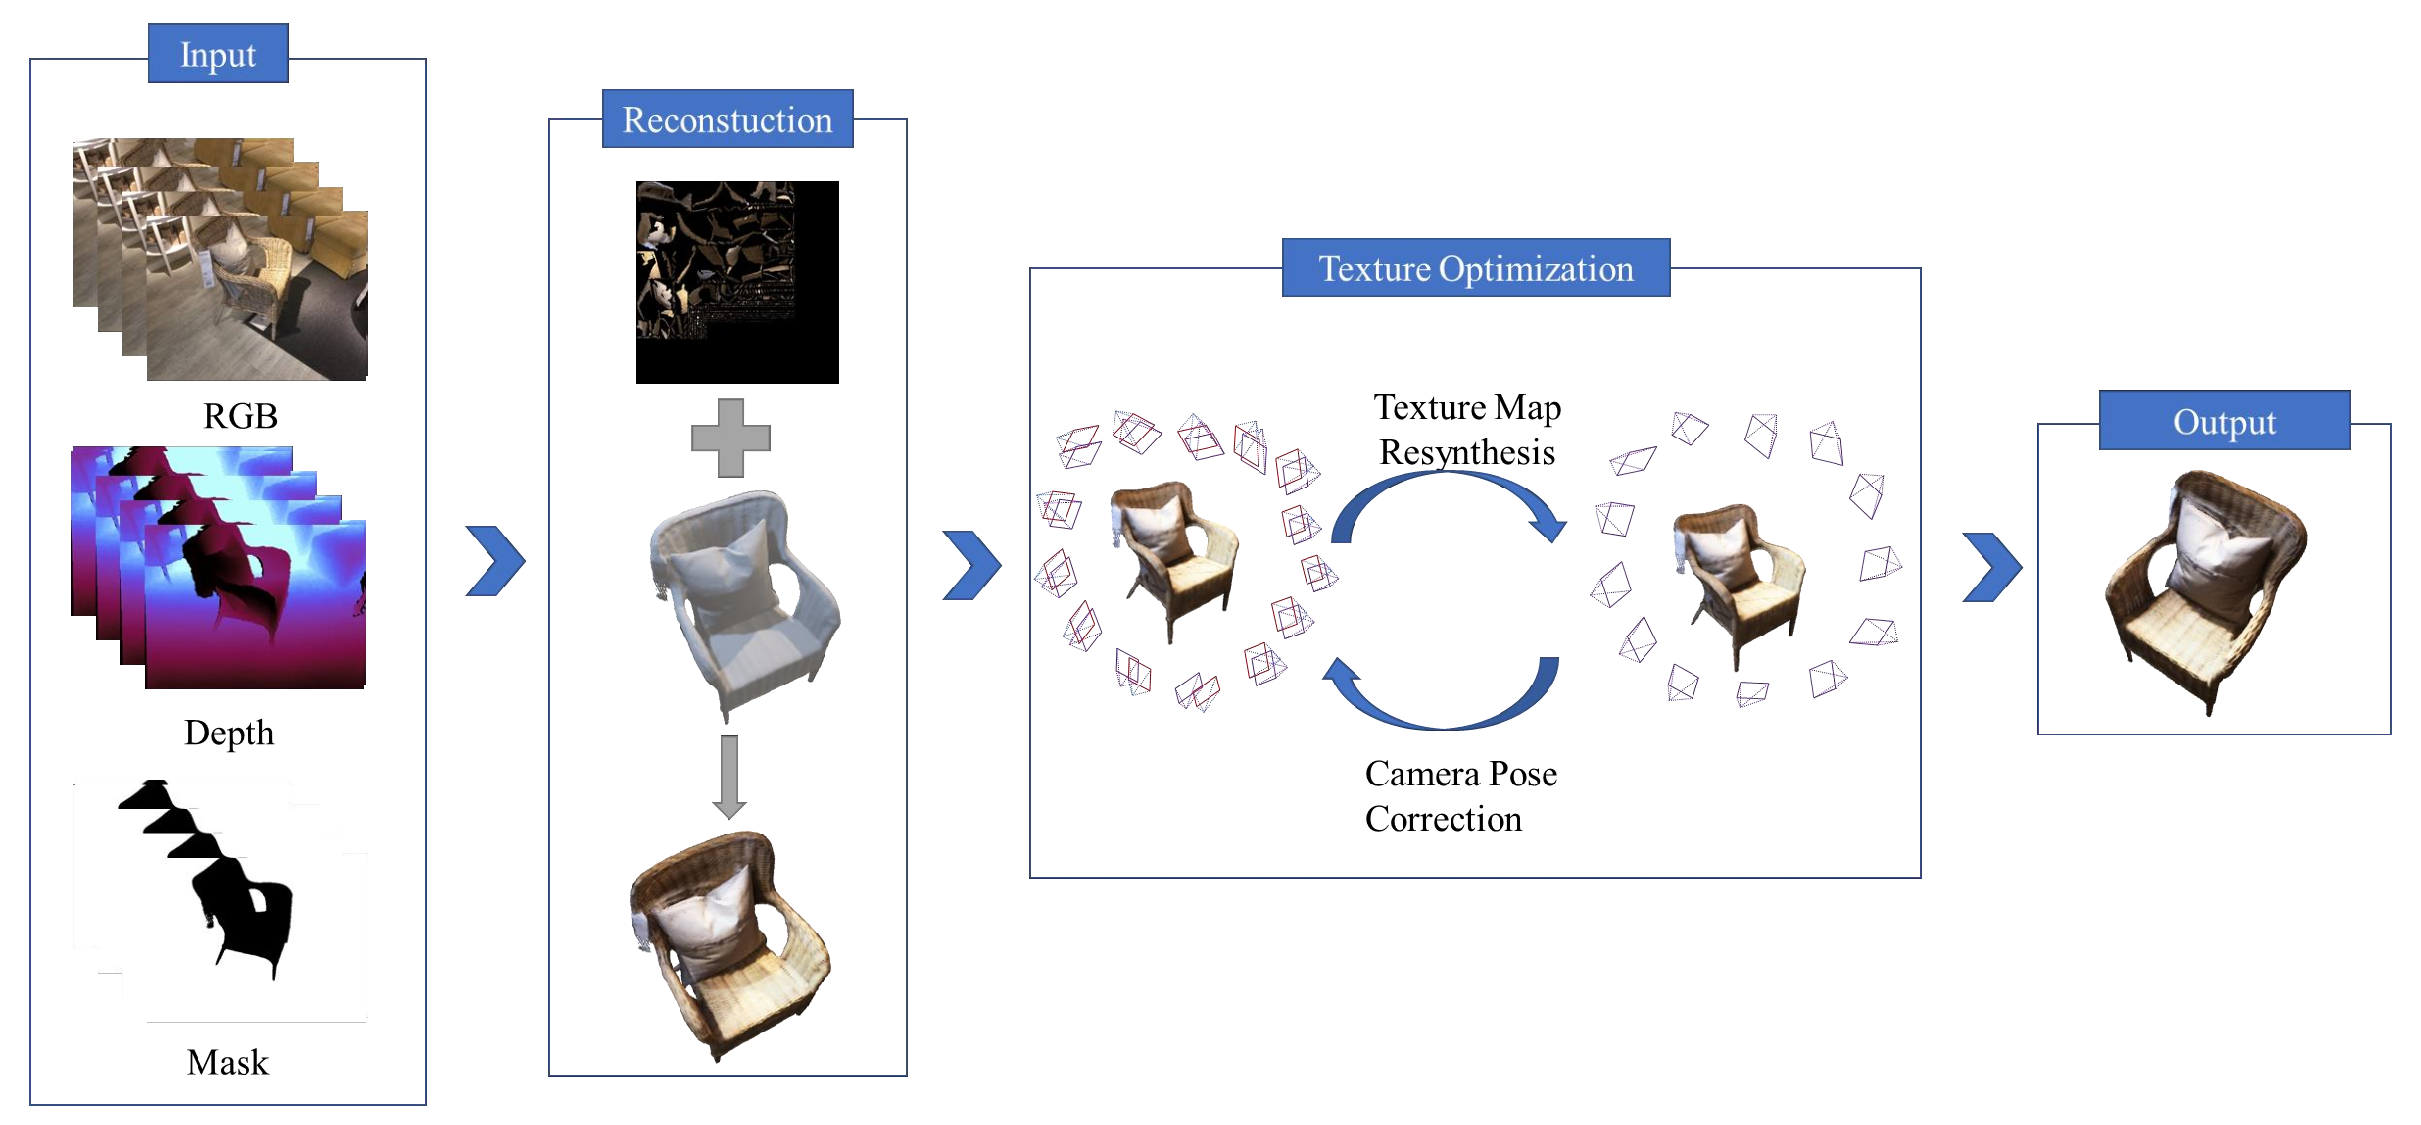
\includegraphics[width=1\columnwidth]{pic/work1/work1.pdf}
    \bicaption{基于可微分渲染的纹理优化概述}{The overview of texture optimization based on differentiable rendering}
    \label{fig:work1}
\end{figure}

本文旨在通过RGB-D相机采集的深度图片和彩色图片,并将不同视角的彩色图适配到几何模型上以生成具高保真的纹理贴图。为了达成这一目标,本文提出结合相机位姿矫正与纹理合成算法提高纹理模型的清晰度和保真度。如图~\ref{fig:work1}所示,算法以彩色图、深度图和相应的掩码图作为输入,通过三维重建得到初始的重建模型。在纹理优化阶段,首先利用可微分渲染矫正相机位姿,接着,利用对抗生成网络合成一幅新的纹理图像,以适配重建模型。具体地、本文的算法分为四个步骤。\par
\noindent\textbf{模型重建:}RGB-D相机采集的原始数据为图片或者视频格式,需要进一步处理转换为同步的的彩色图序列和深度图序列。在公共数据集上,一般会提供深度图集、彩色图集、对应的相机内外参以及用重建算法\upcite{SungjoonChoi2015RobustRO,AngelaDai2016BundleFusionRG,RichardNewcombe2011KinectFusionRD}重建出的初始几何模型。在极少数没有提供几何模型和相机位姿的数据集上,本文通过重建算法\upcite{LongYang2018SurfaceRV}重建初始的几何模型并估计初始的相机位姿。\par
\noindent\textbf{预处理:}在预处理阶段,本文从所有帧中选出最清晰的彩色图像当作候选图像,消除冗余和重叠度较高的视角的影响。同时确保所选关键帧所代表的视角覆盖范围与原始数据集一致。额外采用多视角进行监督,避免单视角因相机漂移导致位姿异常值影响纹理优化过程。具体地,本文为每一帧都选取邻近视角,训练时使用用源视角和扭曲后的视角共同监督。\par
\noindent\textbf{相机位姿矫正:}为了借用可微分渲染框架矫正相机位姿,首先渲染三维模型至某一视角的彩色图像,然后再将真实图像与渲染图像经过损失函数优化相机投影矩阵。矫正相机位姿完成后,再通过将模型的顶点投影至所有可见视角,并采用加权平均算法来融合对应颜色,生成纹理图像。为了便于后续纹理优化,本文将以UV纹理形式保存至二维图像中。\par
\noindent\textbf{纹理优化:}受图像翻译模型\upcite{isola2017image,wang2018high}的启发,本文借助对抗生成网络,以初始纹理为基础生成新的UV纹理。在获取纹理到图像的映射关系和相对准确的相机位姿后,再用源视角$I_A$的邻近视角$I_B$扭曲到源视角当作真例,渲染图像为假例,用对抗生成模型优化纹理图。\par

\subsection{数据预处理}
\noindent\textbf{重建模型:}对于RGB-D数据集,本文使用消费级深度相机kinect \emph{v}1或者kinect \emph{v}2在固定曝光和白平衡模式下拍摄。拍摄完成后,可以得到深度图集和彩色图集以及相机标定后的内参,并没有相机位姿与重建模型。由最近的纹理优化方法G2Tex\upcite{fu2018texture}得到启发,本文也借鉴G2Tex模型重建方案。其初始输入为深度相机扫描的深度图集合和彩色图集合,并借助基于RGB-D三维重建算法\upcite{LongYang2018SurfaceRV}利用稀疏序列融合(Sparse-Sequence Fusion,SSF)的增强策略,获取高可用、高质量的RGB-D序列重建TSDF模型,最后使用移动立方体算法提取出网格模型。重建几何模型的关键帧选取策略依照如下公式进行:
\begin{equation}
E(i)= \lambda_{1} E_{\mathrm{jit}}(i)+\lambda_{2} E_{\mathrm{dif}}(i)+\lambda_{3} E_{\mathrm{vel}}(i)+\lambda_{4}E_{\mathrm{cla}}(i)+E_{\mathrm{sel}}(i)
\end{equation}
其中,$E_{\mathrm{sel}}(i)$表示当前帧$i$是否作为三维重建的有效帧的控制项,$E_{\mathrm{jit}}(i)$用于度量当前帧$i$与上一个有效帧的抖动强度比较,尽量保证选取平滑非抖动帧进行重建,$E_{\mathrm{dif}}(i)$确保前后有效帧间有超过阈值重叠覆盖率,避免相机跟踪失败,$E_{\mathrm{vel}}(i)$度量相机运动速度,避免相机运动过快产生的模糊帧,$E_{\mathrm{cla}}(i)$是图像清晰度度量指标,衡量彩色图片清晰度以保证选择的彩色图像最清晰。经过重建算法后本文得到初始网格模型$M$。\par
\noindent\textbf{关键帧获取。}由于RGB-D相机是手持进行拍摄,拍摄过程中不可避免出现相机抖动或者相机镜头平移速度过快的情况,使得拍摄的图片出现内容模糊、失真等现象。为了根除这个现象,本文会根据 Crete 等人 \upcite{FrederiqueCrete2007TheBE}提出的图片的模糊度度量指标评估每一个彩色帧。对于彩色图超过100张的数据集,本文设置一个大小为5的滑动窗口,在每个窗口内选择模糊度最小的图片作为关键帧$KF$,根据数据集的大小灵活调整窗口大小。经过实验证明选择关键帧并不仅不会影响优化效果而且会线性减少优化时间。 \par
\noindent\textbf{辅助视角选取。}受Huang等人\upcite{JingweiHuang2020AdversarialTO}的启发,本文为每个原始视角$T_s$选取一个辅助视角$T_t$,使得辅助视角重投影至原视角作为真例以此来监督渲染的图片。令$p_s$,$p_t$分别表示原始视角和目标视角的齐次坐标,则二者的对应关系可以描述为:
\begin{equation}
	p_s\sim KT_{t\rightarrow s}D_tK^{-1}p_t \label{work1:wrap}
\end{equation}
其中,$D_t$表示目标视角的深度值。由于遮挡和深度图存在噪声的缘故,目标视口扭曲到原始视角因未对齐会产生残缺现象。为了防止残缺部分过大,本文计算任意两个视口计算z方向夹角$\theta$,当$\theta\le15^{\circ}$时,两个视角加入至源视角-目标视角位姿集合。

\subsection{相机位姿矫正}
\begin{figure}[ht]
    \centering
    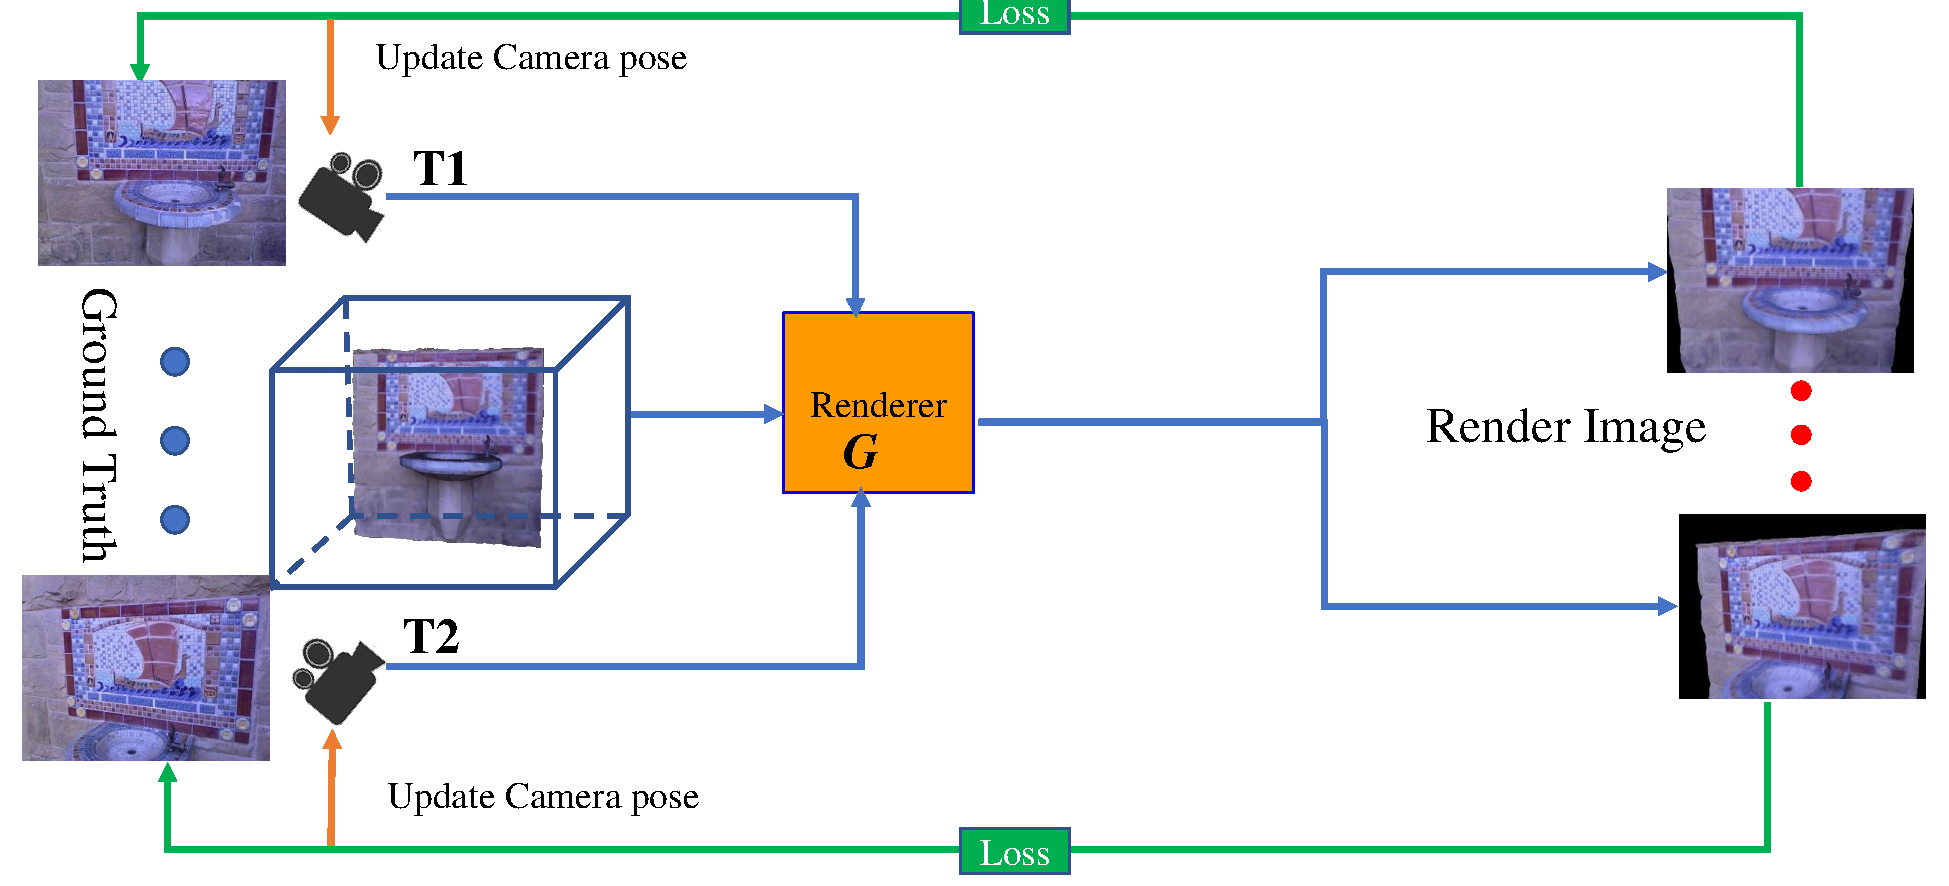
\includegraphics[width=1\columnwidth]{pic/work1/cameras.pdf}
    \bicaption{基于可微分渲染的相机位姿矫正概述}{Overview of camera pose correction based on differentiable Rendering}
    \label{fig:cameras}
\end{figure}

在本节中,本文会详细介绍相机位姿矫正的原理与步骤。如图~\ref{fig:cameras}所示,本文算法的核心在于利用渲染技术渲染模型至不同视角,然后再利用光度一致性误差,产生梯度更新相机位姿矩阵。在模型渲染中,模型会进行刚体变换和透视投影操作。刚体变换的旋转表示有旋转矩阵、欧拉角、轴角表示、四元数等。本文采用旋转矩阵表示,一方面易于向其它表示方式转换,另一方面易于将顶点位置变换到笛卡尔坐标系下。令$ \left \{ \mathbf{I_i} \right \} $表示输入图像集合,$\left \{ \mathbf{T_i} \right \}$表示相机位姿集合,$\left \{ \mathbf{P_i} \right \}$表示图像对应的模型顶点集合。旋转矩阵定义为:
\begin{equation}
	T = \left[\begin{array}{cc}
		R & t \\
		0 & 1
	\end{array}\right]
\end{equation}
$T \in \mathbf{SE}(3)$,$R \in \mathbf{SO}(3)$并且$t\in\mathbb{R}^3$,其中,$T \in \left \{ \mathbf{T_i} \right \}$为4$\times$4矩阵。\par 
将三维重建模型定义在世界坐标系下,并以模型中心为坐标原点。经过刚体变换后,以相机所在位置为坐标原点,模型位于相机正前方。然后,本文采用透视变换将处于相机坐标系下的模型顶点投影至二维图像平面上。根据相机成像模型定义刚性变换为$\mathbf{G}(p)=Tp$,$p \in \left \{ \mathbf{P_i} \right \}$,变换后的顶点齐次坐标为$\mathbf{g}=[g_x, g_y, g_z,g_w]^\top$。设投影图像平面变换为$\mathbf{U}$,本文按照以下公式计算图像平面中的像素位置:
\begin{equation}
\mathbf{U}\left(g_{x}, g_{y}, g_{z}, g_{w}\right)=\left(\frac{g_{x} f_{x}}{g_{z}}+c_{x}, \frac{g_{y} f_{y}}{g_{z}}+c_{y}\right)^{\top} \label{project}
\end{equation}
其中,$f_x,f_y$表示相机在$x,y$方向的焦距长度,$c_x,c_y$分别表示光轴对于投影平面坐标中心的偏移量。这些参数可以利用相机标定获取\upcite{888718}。\par


在基于RGB-D的三维重建中常使用基于三维点云配准的最近邻迭代(Iterative Closest Point,ICP)\upcite{besl1992method,chen1992object}及其衍生算法估计初始的相机位姿。由于存在噪声相机位姿估计存在累积误差,即使后续优化中采用回环检测矫正,也并不能完全消除存在的误差。使用不完美的相机位姿渲染图片,渲染图片和采集图片会发生错位现象。在传统的优化相机方案中,通常计算网格顶点重投影误差来优化相机投影矩阵$T$。设模型上一顶点$p$,初始颜色为$C(p)$(初始颜色,利用顶点投影后的像素颜色平均可得),定义$\Gamma(x,y) $为灰度图像上$(x,y)$位置的颜色值。顶点颜色与投影至视角$i$上的像素颜色值会存在差值,定义残差项为:
\begin{equation}
	R_{i, \mathbf{p}}=C(\mathbf{p})-\Gamma_{i}\left(\mathbf{U}\left(\mathbf{G}\left(\mathbf{p}, \mathbf{T}_{i}\right)\right)\right)
\end{equation} \par
定义优化目标为:
\begin{equation}
	E(\mathbf{T})=\sum_{i} \sum_{\mathbf{p} \in \mathbf{P}_{i}} R_{i, \mathbf{p}}^{2}
\end{equation}

利用高斯牛顿迭代算法\upcite{wedderburn1974quasi}对上述公式进行迭代求解,并且更新一次相机位姿$T$后,重新计算每个顶点的颜色$C(p)$,最终获得精确的相机位姿以及帧间一致的顶点颜色。受传统优化方法得到启发,本文借助于可微分渲染算法投影顶点至图像平面,使用UV纹理保存顶点颜色,通过$L_1$范数度量图像间的颜色差异,最后用梯度下降算法优化相机位姿矩阵$T$。\par
考虑到渲染能力和效率,以及本文无需对模型表面材质进行额外建模,因此使用基于SoftRas的渲染框架\upcite{ravi2020pytorch3d}和布林冯着色模型\upcite{blinn1977models},渲染目标遵从以下规则:
\begin{equation}
	C_i = (I_a + I_d) * P_i + I_s
\end{equation}
其中,$I_a$,$I_d$,$I_s$分别表示环境光系数、漫反射光和高光系数。$C_i$,$P_i$分别表示彩色图像素和纹理像素。为了最大限度的还原具有高保真度的纹理,本文只保留环境光,设置高光和漫反射光系数为0。对于相机外参$T$,本文采用以上介绍的投影和表示方法。渲染框架的所有模块都是可微分的,而且不会增加参数量,因此可以直接作为神经网络的一部分,进行端到端的训练。具体地,每一次渲染本文会随机选择某个视角,在该视角下生成彩色图$\tilde{I}_c$深度图$\tilde{I}_d$以及轮廓图$\tilde{I}_s$,即$\tilde{I}_c,\tilde{I}_d,\tilde{I}_s = Render(M_0|T_i)$。令$I_c, I_d, I_s$分别表示彩色图、深度图和掩码图真值。本文首先使用光度一致性损失来优化已选帧的相机位姿。
\begin{equation}
	E_c = \left \| I_c - \tilde{I}_c  \right \|_1 
\end{equation}

然而,仅仅具有光度一致性损失不足以约束相机位姿以朝着本文期望的方向更新,在某些场景中纹理较为单一或者纹理细节较少时,仍有可能发生相机漂移现象。因此,本文额外考虑深度图损失,以增加几何一致性的约束。
\begin{equation}
	E_d = \left \| I_d - \tilde{I}_d  \right \|_1 
\end{equation}

受SoftRas\upcite{ShichenLiu2019SoftRA}启发,本文也采用轮廓损失来对几何进行约束。这个轮廓损失函数为:
\begin{equation}
	E_s = 1 - \frac{\left \| \hat{I_s}\otimes I_s  \right \|_1 }{\left \| \hat{I_s}\oplus  I_s- \hat{I_s}\otimes I_s \right \| }_1  
\end{equation}
其中,$\otimes $和$\oplus $分别是按元素计算的乘法运算符和求和运算符。最后本文按照各个损失对优化相机参数的贡献来赋予每个损失不同的权重系数。在实验研究中,本文设置权重系数为$\lambda_c = 0.1$,$\lambda_d = 1$,$\lambda_s = 1$。\
\begin{equation}
	L_T = \lambda_c E_c + \lambda_d E_d +\lambda_s E_s \label{pose}
\end{equation} \par

需要注意的是,在不同的场景下,本文可能需要微调优化相关的超参数,而且相机位姿本身没有真实值可供参考。因此,评估相机位姿的准确性唯一的方法是使用矫正后的相机位姿$T'$生成新的纹理图像,并将其与原始纹理进行比较。若新生成的纹理图像越清晰,则说明优化的效果越好。


\subsection{纹理重合成}

\begin{figure}[ht]
    \centering
    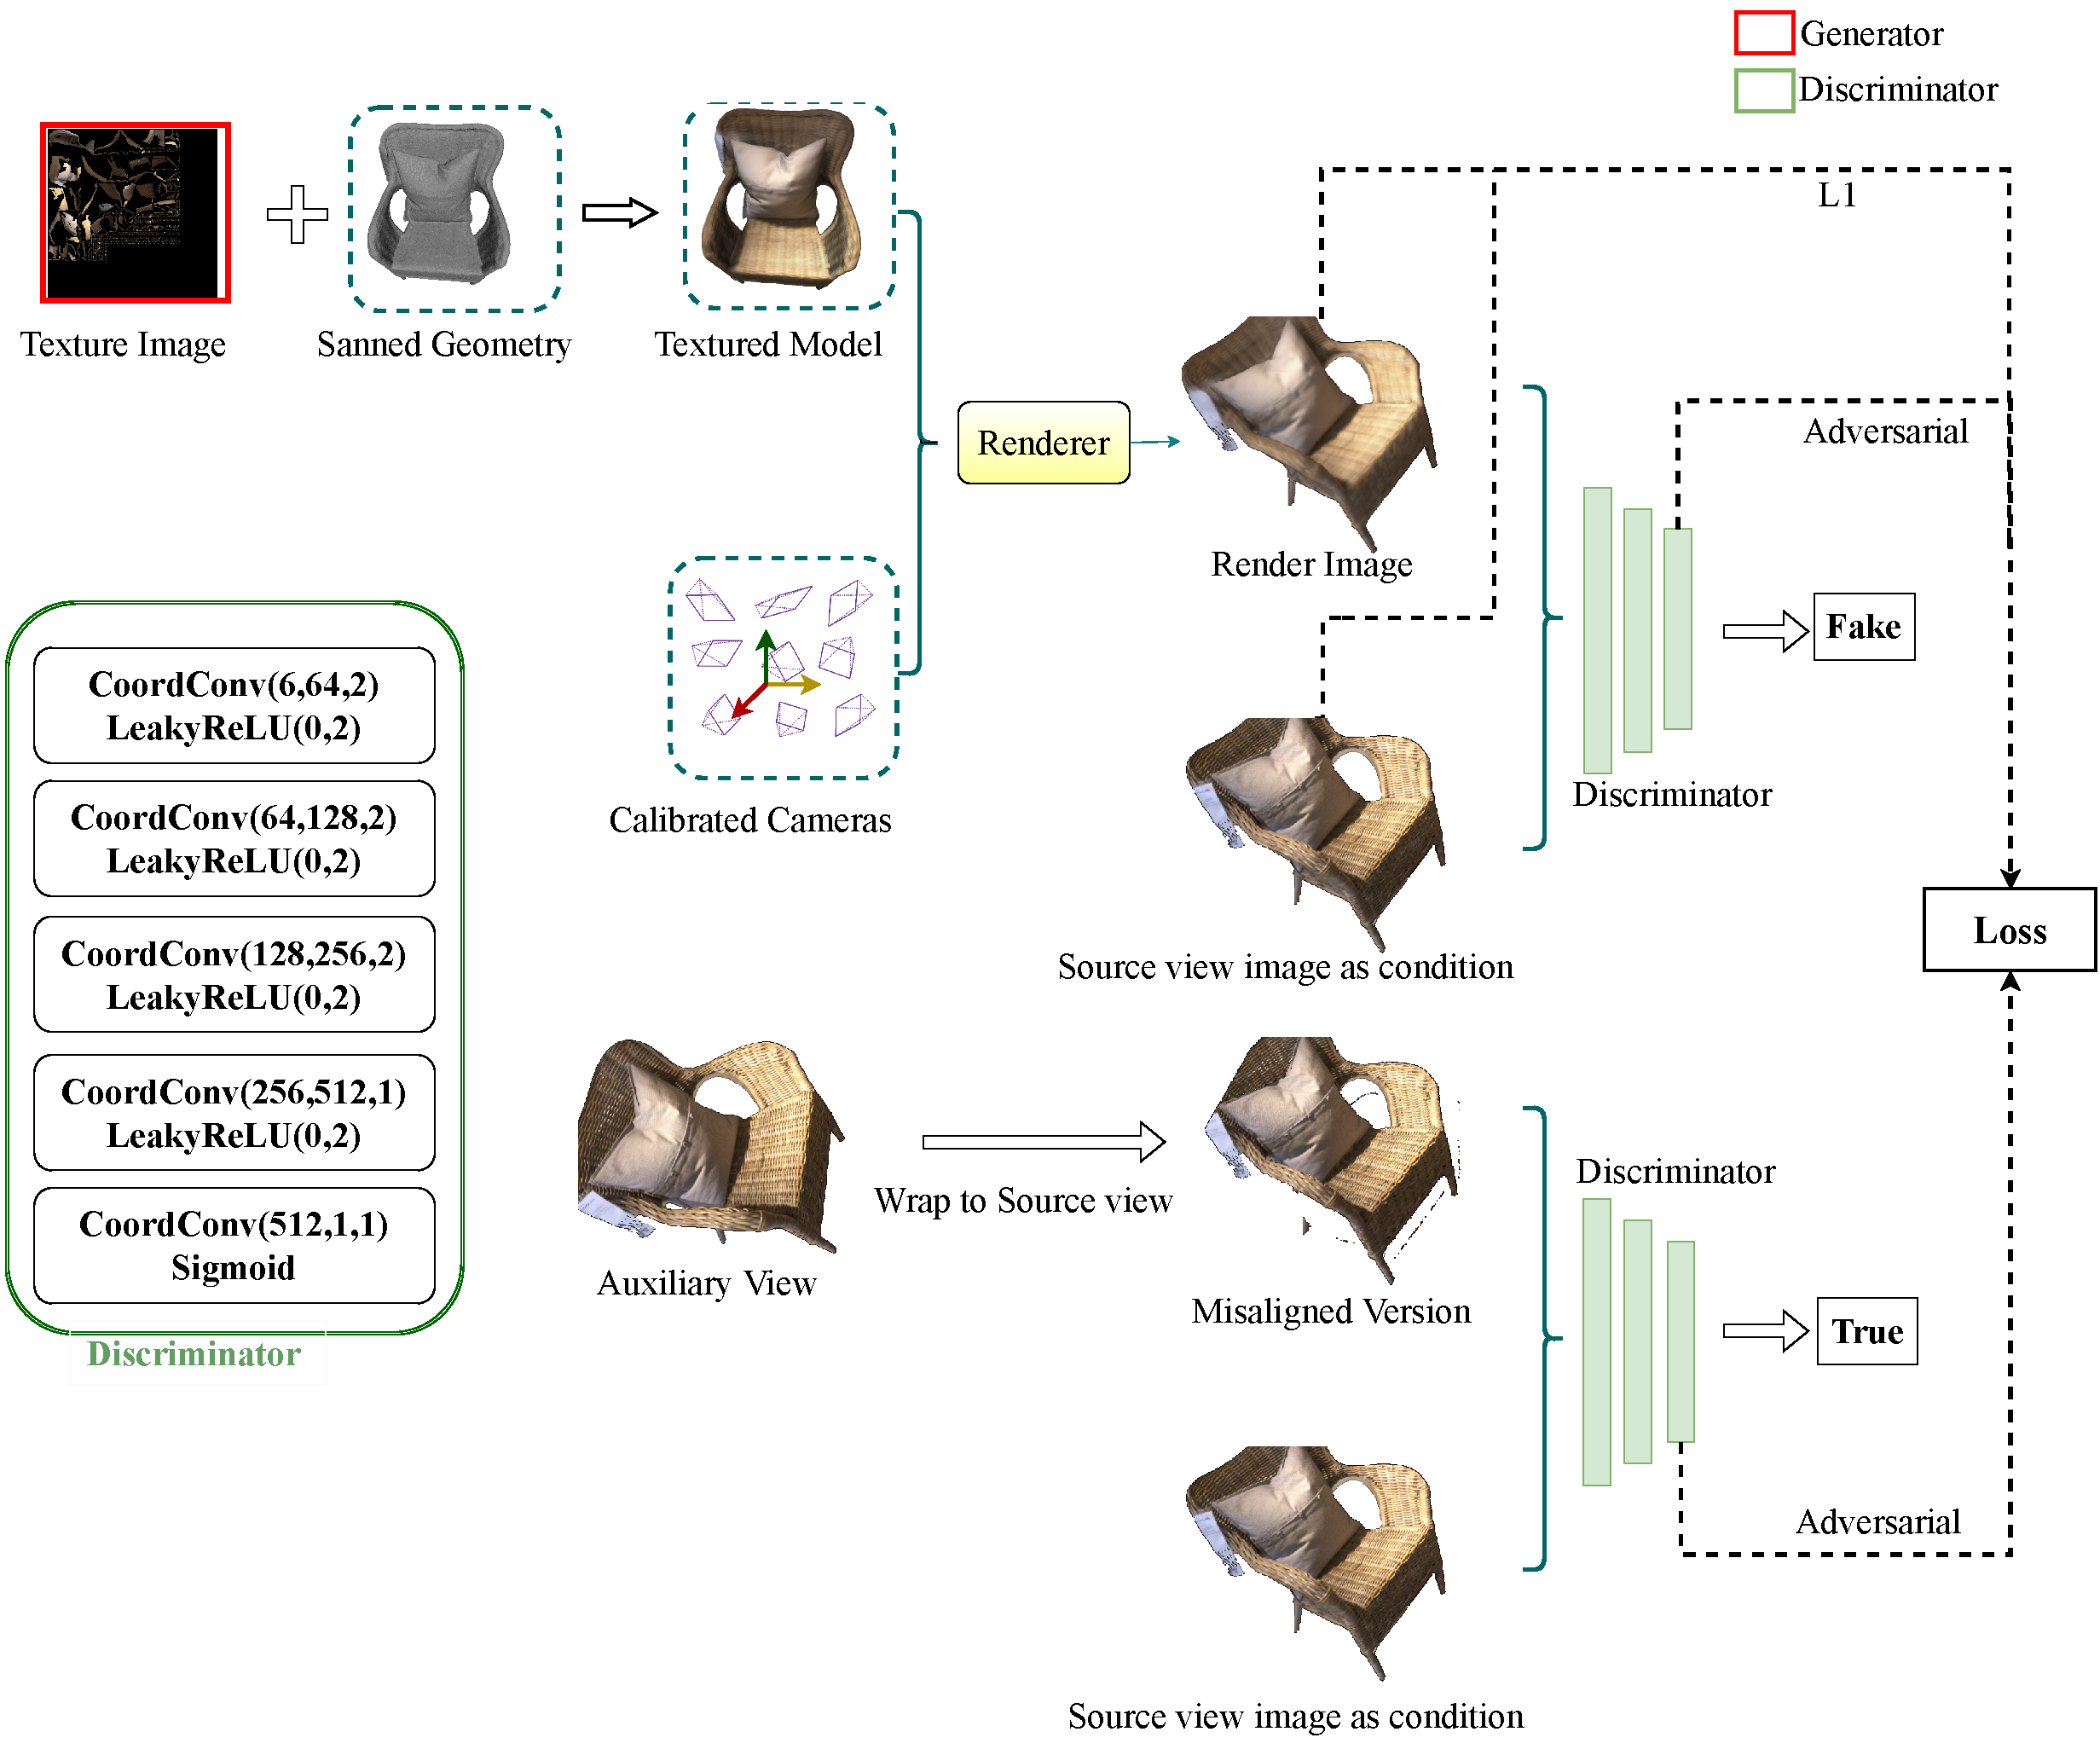
\includegraphics[width=1\columnwidth]{pic/work1/Texture.pdf}

    \bicaption{基于GAN的纹理图像优化概述}{Overview of texture image optimization based on GAN}
    \label{fig:Texture}
\end{figure}

仅仅矫正相机位姿是不够的,优化结果并不能完全消除噪声。传统方法中单纯优化相机步骤后,结果往往需要结合网格细分或者扭曲纹理图像或者纹理坐标,使得进一步使得图像与几何模型对齐,从而抵抗重建模型的噪声以弥补几何误差带来的影响。对于本文的纹理优化算法,本质上也存在这个问题。况且,本文采用顶点加权融合方式生成的纹理,在局部区域会存在模糊并且会丢失细节现象。受到Huang等人\upcite{JingweiHuang2020AdversarialTO}的启发,本文使用对抗生成网络来学习重建模型和拍摄的彩色图片之间错位的容忍度。本文使用基于$\pi$GAN\upcite{chanmonteiro2020pi-GAN,liu2018intriguing}的判别器,通过像素重生成管线合成纹理图。网络结构类似于pix2pix\upcite{isola2017image}的条件对抗网络,利用判别器$D$学习区分真实图片和渲染图片,并产生多视角一致性的纹理图像。本文使用辅助视角重投影至原视角$\boldsymbol{I}_{B \rightarrow A}$为真例,监督可微分渲染生成的彩色图像为假例,以更新纹理图像,并将原始视角的彩色图像作为生成对抗网络的条件。相应地,对抗损失函数定义如下:
\begin{equation}
	L_{a d v}=\log D\left(\boldsymbol{I}_{A}, \boldsymbol{I}_{B \rightarrow A}\right)+\log \left(1-D\left(\boldsymbol{I}_{A},\boldsymbol{I}_{A}^{D R}\right)\right) 
\end{equation}
其中,$\boldsymbol{I}_{A}^{DR}$表示基于源视角的渲染图像。为了使得对抗生成纹理的优化更加稳定,本文额外增加L1损失,避免优化过程陷入局部最小值,并提供初始的指导。L1损失定义如下:
\begin{equation}
L_T = \left \| \boldsymbol{I}_{A}- \boldsymbol{I}_{A}^{D R} \right \| 
\end{equation} \par
 最终本文的优化目标为:
\begin{equation}
	L = L_{adv} + \lambda L_T \label{texture}
\end{equation}

在优化期间,本文设置纹理图像$P$背景像素值为0,$\lambda$为10。每隔1000轮次会指数衰减$\lambda$的数值。\par
具体地,如图~\ref{fig:Texture}所示,对于每一次优化迭代,本文随机选择两个输入图像,$I_A$(源图像,图中所示Source view)和$I_B$(辅助图像,图中所示Auxiliary View),以及对应的相机姿态$T_A$和$T_B$,$I_A$作为GAN网络的条件。“真实图像”为按照公式\ref{work1:wrap}将辅助视角扭曲到源视角后得到图像$I_{B\to A}$(图中所示Misaligned Version)。由于遮挡和相机位姿不准确等因素,$I_{B\to A}$图像会发生残缺现象或者未残缺的部分与源图像$I_A$相比,像素会发生轻微的移位。“伪”图像是根据当前的相机位姿$T_A$从三维纹理模型渲染形成的图像(图中所示Render Image)。纹理的模糊伪影会反映至渲染图像上,判别器识别伪图像和真实图像间的差异,生成器重新生成纹理像素使得渲染图像和扭曲图像充分接近以匹配图像视角与纹理模型的映射关系。在纹理优化过程中,本文通过调整纹理像素的颜色,最大化生成损失,使得纹理图像在判别器视角下看起来更逼真。在判别器优化过程中,本文最小化对抗性损失,降低假样本与真样本之间的概率分布差异。最后,本文对总损失与L1损失函数进行线性组合,提高纹理优化效果。\par
经过若干次迭代交替训练判别器$D$和纹理$P$后,判别器会正确识别渲染图片中存在的伪影模糊或者裂缝现象,纹理图像会被重新生成,以弥补渲染图片和真实图片之间错位,使两者充分接近,达到欺骗判别器的目的。经过优化后的纹理相比与用加权融合方法生成的纹理更加真实,更接近于真实拍摄的彩色图片。\par


\subsection{迭代优化}

本文并未将优化方法和合成方法集成到一个模型中。相反,本文采用交替优化方案,以寻找生成最佳纹理。一般来说,矫正相机位姿和对抗生成网络合成纹理顺序可以交换,但是本文实验研究发现,先矫正相机姿态有助于提高纹理的保真度。一方面,相机位姿是纹理映射的核心,若相机位姿完全无误差,则不同视角直接贴在几何模型中就可以生成完美的纹理图。换句话说,位姿对纹理生成的影响最大。另一方面,合成纹理图也依赖于位姿变换,位姿越准确,合成效果越好。在外部迭代中,本文矫正相机位姿后再合成纹理模型,并且整个优化过程重复$N$次。在内部迭代中,本文根据不同场景设置相机位姿迭代次数$S_1$,纹理优化迭代次数$S_2$。一般情况下,本文设置$N \le 3,S_1 \le 40,S_2 \le 4000$,即可生成清晰的纹理图像。

\section{实验结果与讨论}
\paragraph*{\textbf{比较方法}}
在这个部分,本文会在公开的RGB-D数据集上,通过和以合成法为代表的纹理优化方法ATO\upcite{JingweiHuang2020AdversarialTO},以及以优化法为代表的纹理优化方法Zhou\upcite{zhou2014color},并使用他们在GitHub提供的源代码进行比较。由于Zhou采用顶点颜色加权融合方法生成纹理映射结果,最终结果以顶点颜色存储。这与本文和ATO使用UV纹理的纹理表示方案不同,其生成纹理的清晰度与顶点数目成正相关。为了公平起见,本文按照Zhou的选帧策略,选取最清晰的帧作为关键帧,并使用三角形中点细分方法对重建模型细分两次,以增加顶点数目。最后,设置优化轮次为关键帧数目的10倍。其它超参数均按照源代码给定的设置。本文在不同数据集的多个场景中进行了定性及定量实验分析,证明了本文方法的有效性。数据集既包含小场景,也包含大场景,既包含了含有丰富纹理细节的场景,也包含了单一纹理及弱纹理的场景。最后,本文将展示消融研究结果,以证明本文优化方案中各个组件的必要性。\par
% \paragraph*{\textbf{评估指标}}
\noindent\textbf{评估指标}\quad
为了对所生成的纹理进行定量研究,本文采用多种指标来衡量生成纹理与真实图片之间的差异。目前,纹理优化结果并没有一种行之有效的定量评估指标。一方面,因为大部分纹理映射算法会采用wrap图像的方法以适配几何模型,导致渲染图像无法完全与采集图像对齐。仅使用图像间的评估指标有待商榷。另一方面,纹理映射结果的表示形式多样,没有一个通用的标准形式。因此,评估纹理映射的好坏主要以\textbf{定性}比较为主。但是,定量评估指标能够在一定程度上反映纹理图像的清晰度和保真度。本文使用经典的图像间评估指标来进行定量分析,如峰值信噪比(Peak Signal-to-Noise Ratio,PNSR)\upcite{de2003improved}用于量化受损压缩影响的图像,能够反映图像的保真度,结果越高代表重建图像质量越好;结构相似性指数(Structural Similarity Index,SSIM)\upcite{brunet2011mathematical}是一种评价两张图片相似度的指标,它综合考虑了图片的亮度、对比度和结构信息,符合人类对图像的视觉感受,评价结果越高越好;学习感知图像块相似度(Learned Perceptual Image Patch Similarity,LPIPS)\upcite{zhang2018unreasonable}也称为感知损失,以神经网络计算误差的方法度量两张图像之间的差别,更符合人类的感知,其结果越小越好。在定量评估方面,首先渲染纹理模型至不同视角,并使用所有视角的结果的平均值来作为最终结果。


%\paragraph*{\textbf{训练设置}}
\noindent\textbf{训练设置}\quad
本章方法使用Ubuntu 18.04 LTS进行训练和测试,显卡为单个NVIDIA GeForce RTX3090 24GB,在训练网络时使用Adam优化器训练模型,并设置超参数$\beta_1=0.5,\beta_2=0.999,\epsilon =10^{-8}$。在矫正相机位姿时设置初始学习率为0.0001,用对抗生成优化纹理时设置初始学习率为0.01。


\begin{figure}[!t]
\centering
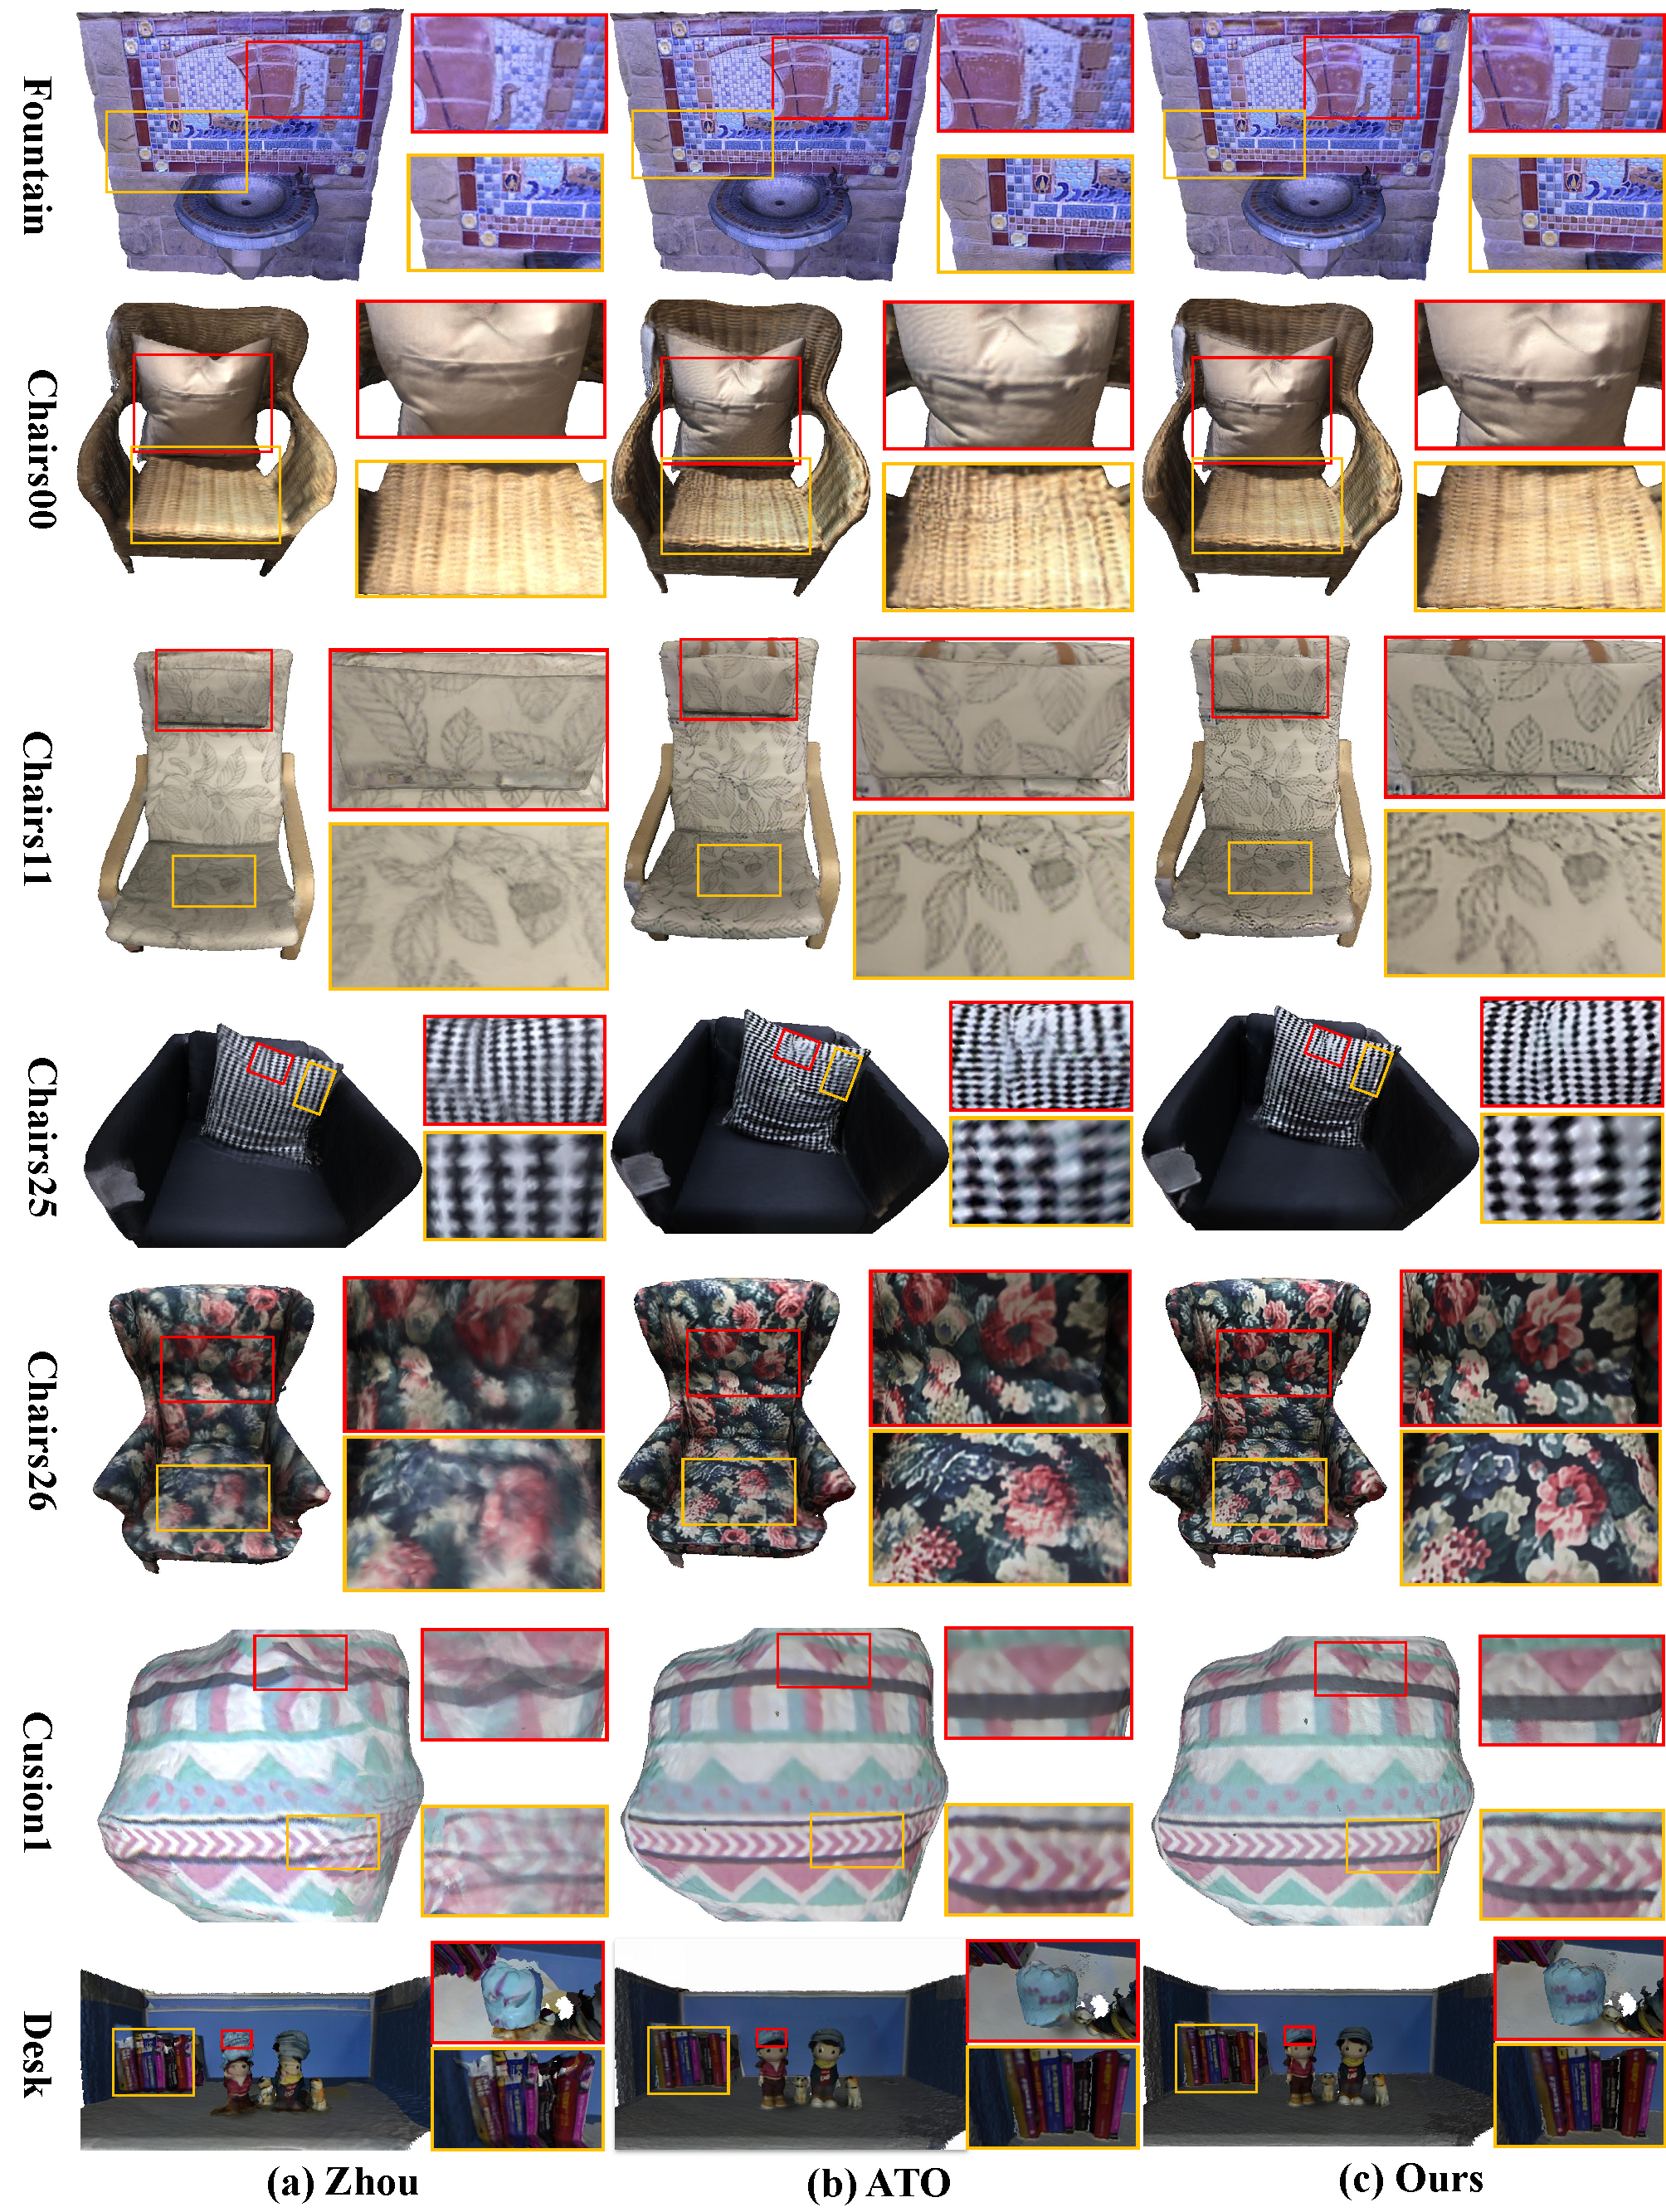
\includegraphics[width=1\linewidth]{pic/work1/visual.pdf}

\bicaption{公共数据集上不同方法的定性比较}{Qualitative comparison of different methods on public datasets}
\label{fig:ex1_1}
\end{figure}

\subsection{公共数据集上结果与分析}
本文首先在ATO\upcite{JingweiHuang2020AdversarialTO}发布的椅子数据集上数据集上进行实验比较。如图~\ref{fig:ex1_1}第二三四行所示,可以看出本文的方法得到了最佳的视觉效果,ATO采用对抗神经网络方法合成纹理图,虽然能够容忍较小的相机误差和几何误差,但是在局部地方仍然有模糊现象。例如,在$\emph{Chairs00}$ 场景下(图第一行)红色框所标注的枕头细节。本文方法与Zhou在枕头表面纹理更加平滑,不会含有噪声。在$\emph{Chairs11}$场景下,本文方法比起Zhou与ATO更加凸显椅子树叶图案的细节,如第三行红色框所展示内容。单纯的对抗生成大体上能合成貌似真实的结果,但是在相机位姿误差影响下干扰了神经网络合成图像细节的能力,这一点在纹理更加丰富的$\emph{Chairs26}$场景下更加明显。从图中橙色和红色框标注的内容上可以看出,虽然ATO纹理合成结果相比于Zhou显著减小了模糊程度,更加贴近真实结果。但是仍旧会存在伪影现象。从结果上看,本文成功地将纹理映射中的模糊伪影影响降至最低。如图第四行,在\emph{Chairs25}场景下,虽然ATO可以生成整体效果较好的纹理图像,但是在局部区域却出现了非常明显的模糊现象,导致原本清晰的黑色线条变得杂乱不清。Zhou采用顶点颜色融合方法生成纹理,当某些顶点投影位置错误时会影响加权结果导致纹理模糊,在纹理较为单一场景如$\emph{Chairs00}$与$\emph{Chair11}$下问题并不明显,但是在图案比较明显的$\emph{Chairs26}$场景下,瑕疵十分明显。例如,该场景下橙色框所展示的花瓣,图片颜色上没有区分度,局部细节存在模糊现象。本文也在Zhou发布的数据集$\emph{Scene3d}$,其中最具代表性的$\emph{Fountain}$场景下进行对比,相比于$\emph{Chairs}$数据集下的场景,该场景的视角非常稀疏,对依赖于大量数据训练的ATO与本文方法带来新的挑战。从最终结果看本文的纹理映射结果整体效果最好,无论是恢复瓷砖表面的细节(图片红色框展示)还是生成墙壁上的字体(图片橙色框展示)方面,更符合真实场景。而Zhou与ATO纹理映射结果要么存在模糊伪影,要么缺乏纹理细节。由于本文先矫正了相机位姿,为模型提供了更正确的纹理映射,又采用对抗生成方法增强纹理高频细节,所以无论从整体还是局部更符合真实场景。\par

为了证明本文在微小模型下,复杂场景下也能恢复出高保真的外观模型。本文采用Fu等人\upcite{fu2018texture}发布的数据集上进行评估。该数据集用Kinect一代相机拍摄的数据集,它获得的深度图和彩色图的分辨率较低 (640 $\times$ 480),更容易受到运动模糊,相机抖动的影响。而且获得的彩色图像中物体几何特征和色彩细节并不明显。同时该数据集上存在阴影、光照等其它噪声,相机位姿相比于$\emph{Chairs}$,$\emph{Fountain}$存在更多噪声。从图中后三行所示,Zhou只能保证场景下整体效果,但是局部细节普遍存在瑕疵。一方面源于重建模型不精确,经过中点细分又加剧了几何误差的影响。另一方面,Zhou用高斯牛顿矫正相机位姿,非刚性优化矫正内参。相比于Adam优化器\upcite{kingma2014adam}优化时梯度下降更易陷入局部最小值,残差项减小的更慢,影响了优化效果。如图$\emph{Cusion1}$场景中的黑色线条存在重影现象;$\emph{Desk}$场景下左边人物帽子未能正确产生纹理映射效果。ATO在三个场景下能生成正确纹理映射结果,但是某些细节处的伪影未能完全根除。例如,在$\emph{Bolster1}$橙色框所示图案,$\emph{Desk}$场景下人物帽子上的字体细节,人物旁边书籍名称等。本文方法相比于ATO与Zhou无论是整体视觉效果还是局部细节均展示了本文方法的优越性。\par

最后本文采用定量分析法,对整个纹理模型渲染的图像用上述介绍的评估指标进行定量分析,结果如表~\ref{tab:evluation_ex2}所示。其中G2TeX包含$\emph{Bloster1}$、$\emph{Cusion1}$、$\emph{Desk}$三个场景,$\emph{Scene3d}$包含$\emph{Fountain}$一个场景,$\emph{Chairs}$包含$\emph{Chairs00}$、$\emph{Chairs11}$、$\emph{Chairs26}$三个场景。以上所有指标均为所有场景下,不同视角渲染图片得到的度量平均值。从结果上看,本文的指标高于两者,说明纹理优化中相机位姿矫正的必要性。

\begin{table}[ht]
\bicaption{公共数据集上不同方法的定量比较}{Quantitative comparison of different methods on public datasets}
\renewcommand{\arraystretch}{1.3}

\label{tab:evluation_ex2}
	\centering
    \scalebox{0.9}[1]{
		\begin{tabular}{lcccccccccc}
            \hline
			{Datasets} & \multicolumn{3}{c}{G2Tex (3 models)}  &\multicolumn{3}{c}{Scene3d (1 models)} & \multicolumn{3}{c}{Chairs (3 models)}\\
			{} & PSNR$\uparrow$ & SSIM$\uparrow$ & Perceptual$\downarrow$ & PSNR$\uparrow$  & SSIM$\uparrow$ & Perceptual$\downarrow$ & PSNR$\uparrow$ & SSIM$\uparrow$ & Perceptual$\downarrow$ \\
			\hline
			zhou & 22.758 & 0.920 & 0.070 & 21.684 & 0.649 & 0.276 & 17.637 & 0.583 & 0.287 \\
			ATO & 23.734 & 0.941 & 0.058 & 25.463 & 0.770 & 0.269 & 21.235 & 0.680 & 0.250 \\
			Ours & \textbf{25.185} & \textbf{0.949} & \textbf{0.042} & \textbf{26.716} & \textbf{0.793} & \textbf{0.251} & \textbf{21.462} & \textbf{0.696} & \textbf{0.247} \\
            \hline
		\end{tabular}
		}
	\normalsize
\end{table}

%%
% 分别研究损失函数、仅深度图、仅彩色图。分别研究没有优化相机位姿、没有对抗生成网络情况,并添加随机噪声结果
%
\subsection{消融实验}
\begin{figure*}[ht]
\centering
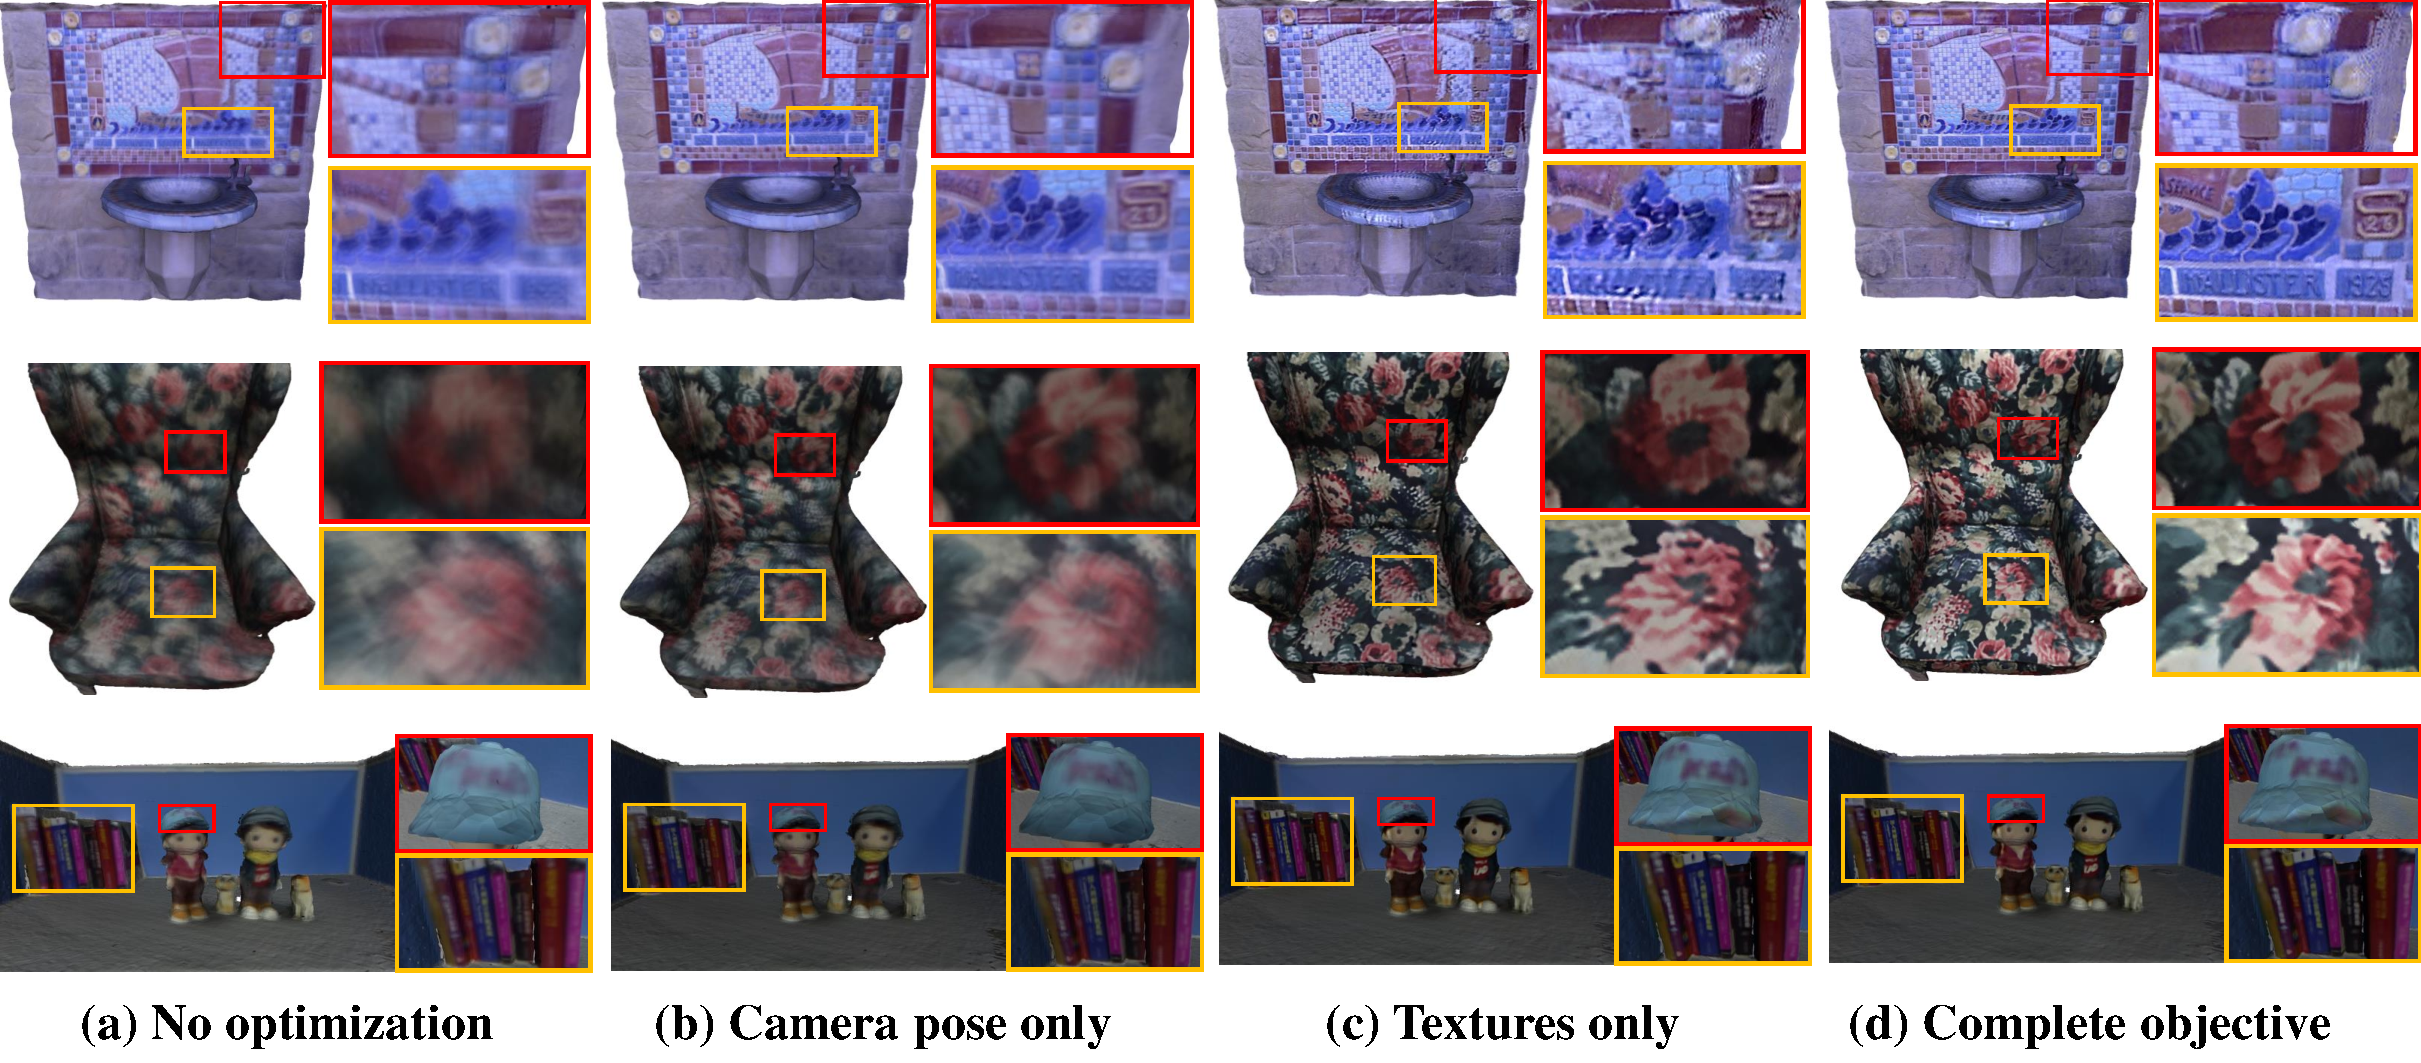
\includegraphics[width=1\linewidth]{pic/work1/final.pdf}
\bicaption{消融实验中纹理渲染结果定性比较}{Qualitative comparison of texture rendered results in ablation study}
\label{fig:ex1_2}
\end{figure*}
在这个部分,本文将研究方法中各个部分的有效性。为了更有说服力,本文选择纹理更加丰富,视觉效果强烈的$\emph{Fountain}$、$\emph{Chairs26}$、$\emph{Desk}$场景。本文分别在只矫正相机位姿,只使用对抗生成网络以及联合优化情况下展示定性结果比较。\par
如图~\ref{fig:ex1_2}所示,本文首先展示了使用图像反向投影至几何模型上生成的初始纹理映射模型(如图第一列)。在没有任何优化的情况下,视觉效果非常模糊。如图第二列所示,若没有矫正相机位姿,则渲染图片和真实图片会出现错位现象。仅仅使用可微分渲染矫正相机位姿,可以减少纹理模糊的程度,但是无法增强图像亮度、对比度等纹理细节。没有对抗生成网络时,无论是纹理细节还是整体视觉效果相比于最终结果明显下降。仅使用对抗生成网络,则可以显著提升纹理清晰度和保真度,但是存在和ATO一样的方法缺陷。本文通过矫正相机位姿,为对抗生成网络合成纹理图片寻找正确的优化方向。本文在定量评估表~\ref{tab:ablation1}中也得出了相同的结论。\par
\begin{table}[h]
\renewcommand{\arraystretch}{1.3}
\bicaption{消融实验中纹理渲染结果定量比较}{Quantitative comparison of texture rendered results in ablation study}
\label{tab:ablation1}
	\centering
%    \scalebox{0.80}{
		\begin{tabular}{lcccc}
			\hline
			{Methods} & \tabincell{c}{No pose \\ correction} &\tabincell{c}{No adversarial \\ loss} & \tabincell{c}{Complete \\ method} \\
			\hline
			PSNR$\uparrow$ & 18.515 & 24.763 & \textbf{25.330}\\
			SSIM$\uparrow$ & 0.710  & 0.764 & \textbf{0.764}\\
			Perceptual$\downarrow$ & 0.094  & 0.043 & \textbf{0.043}\\
			\hline
		\end{tabular}
%	}
%	\normalsize
\end{table}


\subsection{算法局限性}
本文的优化算法虽然已经取得了一定的成效但是仍旧有以下不足的地方。
\begin{enumerate}[label=(\arabic*),leftmargin=\parindent,align=left,labelwidth=\parindent,labelsep=0pt]
\item 无法自定义纹理坐标。本文使用\emph{obj}格式保存三维模型,需要额外存储纹理坐标以表示几何与纹理图像(UV纹理)的映射关系。\emph{ply}存储格式转为\emph{obj}格式时需要额外生成纹理坐标,但本文算法不包含纹理坐标产生流程,限制了算法通用性。
\item 需要更多的数据。本文主要使用基于深度学习的方法更新相机位姿和纹理图像,因此需要大量的训练数据来进行模型的更新。相比传统方法只需要覆盖 $360^{\circ} $ 的图像,本文需要更多的数据来获得最佳效果。在使用较小的数据集上,本文的优化效果可能会受限制,这限制了本文在小场景下的应用。
\item 在某些场景下,几何模型可能存在许多误差,即使优化纹理图像也无法保证其正确的映射关系。特别是在几何模型存在孔洞和非流形拓扑结构的情况下,这一现象将更加常见。
\end{enumerate}





\section{本章小结}

针对基于RGB-D三维重建产生的模糊纹理问题,本文提出了针对RGB-D三维重建模型的相机位姿矫正与纹理重合成结合的纹理优化算法。首先,本文输入三维重建的模型与采集得到的图片序列及其对应视角的相机位姿参数,用可微分渲染方法渲染纹理至图像,并使用重投影误差产生梯度更新相机投影矩阵;然后,用对抗生成网络重新合成新的纹理图像以适配重建模型;最后,输出一个完整且全局一致的纹理模型。实验结果表明本文的算法在大场景、小场景、在含有丰富纹理细节和含有弱纹理场景下,都能恢复出高保真的纹理,也证明了本文算法的高通用性和强鲁棒性。





% 第四章工作二
% \clearemptydoublepage
% \setcounter{figure}{0}
% \setcounter{tableEng}{0}
% \setcounter{algocf}{0}
% \chapter{基于网格自适应细分的几何与纹理优化}


\chaptera{基于网格自适应细分的几何与纹理优化}
\section{引言}

由于消费级深度相机的广泛普及,3D场景的重建得到了极大的关注。借助于深度相机人们能够很容易的对真实世界的场景进行建模得到场景和物体的三维模型,基于深度(RGB-D)相机的静态场景\upcite{RichardNewcombe2011KinectFusionRD,ThomasWhelan2012KintinuousSE,ThomasWhelan2015ElasticFusionDS,SungjoonChoi2015RobustRO,VictorAdrianPrisacariu2017InfiniTAMVA,AngelaDai2016BundleFusionRG}和动态场景重建\upcite{newcombe2015dynamicfusion,innmann2016volumedeform,yu2017bodyfusion,yu2018doublefusion,xu2019unstructuredfusion,su2020robustfusion,slavcheva2017killingfusion,gao2019surfelwarp,dou2016fusion4d}技术也发生了前所未有的进步。然而,三维重建结果无法满足虚拟现实、混合现实、动画、影视、游戏等领域的需求,一方面是重建几何模型存在瑕疵;另一方面,即使几何模型结果满足基本需求模型外观也无法达到与照片相媲美的程度,很难使人满意也无法直接应用。\par

要获得高保真的纹理映射模型,需要满足两个标准:精确的重建模型和清晰且全局一致的纹理。然而,实际应用中这两个标准常常受到以下因素的干扰。首先,深度相机采集的深度并非绝对准确,当测量距离大于一定阈值时会存在大量误差,并且室内光源的影响也会增加测量误差。其次,在几何模型的三维重建过程中,现有算法为了抵御噪声会使用加权平均方法,这会抹去几何模型的高频细节,使得重建模型整体较为完美但在细节处存在瑕疵。最后,多种误差因素相互叠加,即使采用回环矫正、位姿图优化等算法,相机位姿也只能保证相对准确。这些因素综合影响了图像和几何模型的准确对齐,获取高质量、高保真的纹理映射就需要做进一步的优化。\par


先前的工作采用各种方法试图解决以上所述问题,一般通过合成纹理图像\upcite{bi2017patch}、矫正相机位姿\upcite{zhou2014color}或者细分网格顶点\upcite{ChengleiWu2014RealtimeSR}方面,生成更高质量的三维模型。有的工作不止着眼于单个组件的优化,在先前工作基础上额外提出优化策略使得纹理映射结果更加逼真。如G2Tex\upcite{fu2018texture}采用在基于面投影方法上额外使用从全局到局部的相机位姿矫正方案,成功消除了纹理边界处的大量细缝,生成照片级纹理图像取得了良好的效果。Seamless\upcite{fu2021seamless}也采用面投影方式,并额外采用块合成的方法在纹理边界处重新合成图案以消除纹理。大部分工作聚焦于如何改进或者生成纹理图像以弥补重建模型的误差,但是补偿能力有限,并且只适用于重建模型误差较小情况,未考虑纹理、相机位姿、几何模型之间的耦合性关系,在优化场景的选择上有限制。Intrinsic3D\upcite{RobertMaier2017Intrinsic3DH3}是首个基于明暗变化恢复形状(Shape From Shading,SFS)方法,对场景中的模型形状、模型颜色、相机位姿以及场景光照进行联合优化,但是由于SFS方案会产生纹理复制现象制约了Intrinsic3D方法的应用。最近Fu等人提出JointTG\upcite{YanpingFu2020JointTA}方案对几何、相机位姿、纹理分别进行迭代优化,再采用分层方案代替混合优化策略成功解决Intrinsic3D纹理复制问题并且速度更快。然而,该方案的复杂框架针对不同的优化方案和目标函数进行分别设计,因此在可扩展性和健壮性方面存在一定的挑战,特别是在重建误差较大的情况下。\par

受可微分渲染在三维单视图模型重建\upcite{liu2020general,ShichenLiu2019SoftRA}中的成功启发,本文
提出了一个基于可微分渲染的联合优化深度学习框架,用于同时优化相机位姿、纹理和几何模型。克服现有只对一个因素进行优化而难以达到全局最优解的障碍,并最终得到带有清晰的纹理与精细几何细节的三维重建结果。该框架的核心是一个可微分渲染模块,该模块需要共同参与纹理模型渲染至图像的几何模型、纹理和相机位姿,因此梯度可以在各个组件之间进行传递更新。该框架使用共同的图像间损失函数来优化不同的组件,并具有较高的可扩展性和灵活性。此外,为了突出恢复模型的高频细节,本文还引入了自适应质心细分方法,即仅在纹理丰富区域细分几何模型,以优化几何模型的细节。为了加快模型的收敛速度和优化效果,本文提出了一个交替优化方案,该方案采用分层迭代更新每个组件,从而提高模块的灵活性和训练过程的稳定性。最终,本文成功重建了带有清晰纹理和精细几何细节的三维模型。\par

本文的实验表明,与最先进的方法相比,本文的联合优化框架相比于最新纹理优化方法在真实数据上的可视化结果表现优异。展示了本文在恢复出三维重建模型高频几何细节和表面纹理方面具有优势。\par
总的来说,本章主要包括以下几个贡献:\par
\begin{enumerate}[label=(\arabic*),leftmargin=\parindent,align=left,labelwidth=\parindent,labelsep=0pt]
\item 本文提出了一种基于可微分渲染的全新联合优化方案,将几何模型、纹理图像和相机位姿统一放置于同一框架内,对每个组件分别进行交替优化,最终实现高质量的三维几何模型和高保真的纹理图像。
\item 本文采用对抗生成网络以增强纹理图像的真实感。此外,设计的渲染模块可以灵活嵌入到神经网络中,并且可以自由选择网络结构和优化方式,使整个系统具有高度的可扩展性。
\item 在网格顶点的优化过程中,本文提出了一种自适应细分方法,该方法仅在纹理丰富区域进行细分,可以有效减少计算代价,同时实现与全局细分相同的效果。
\end{enumerate}

\section{算法流程}
\begin{figure}[!t]
    \centering
    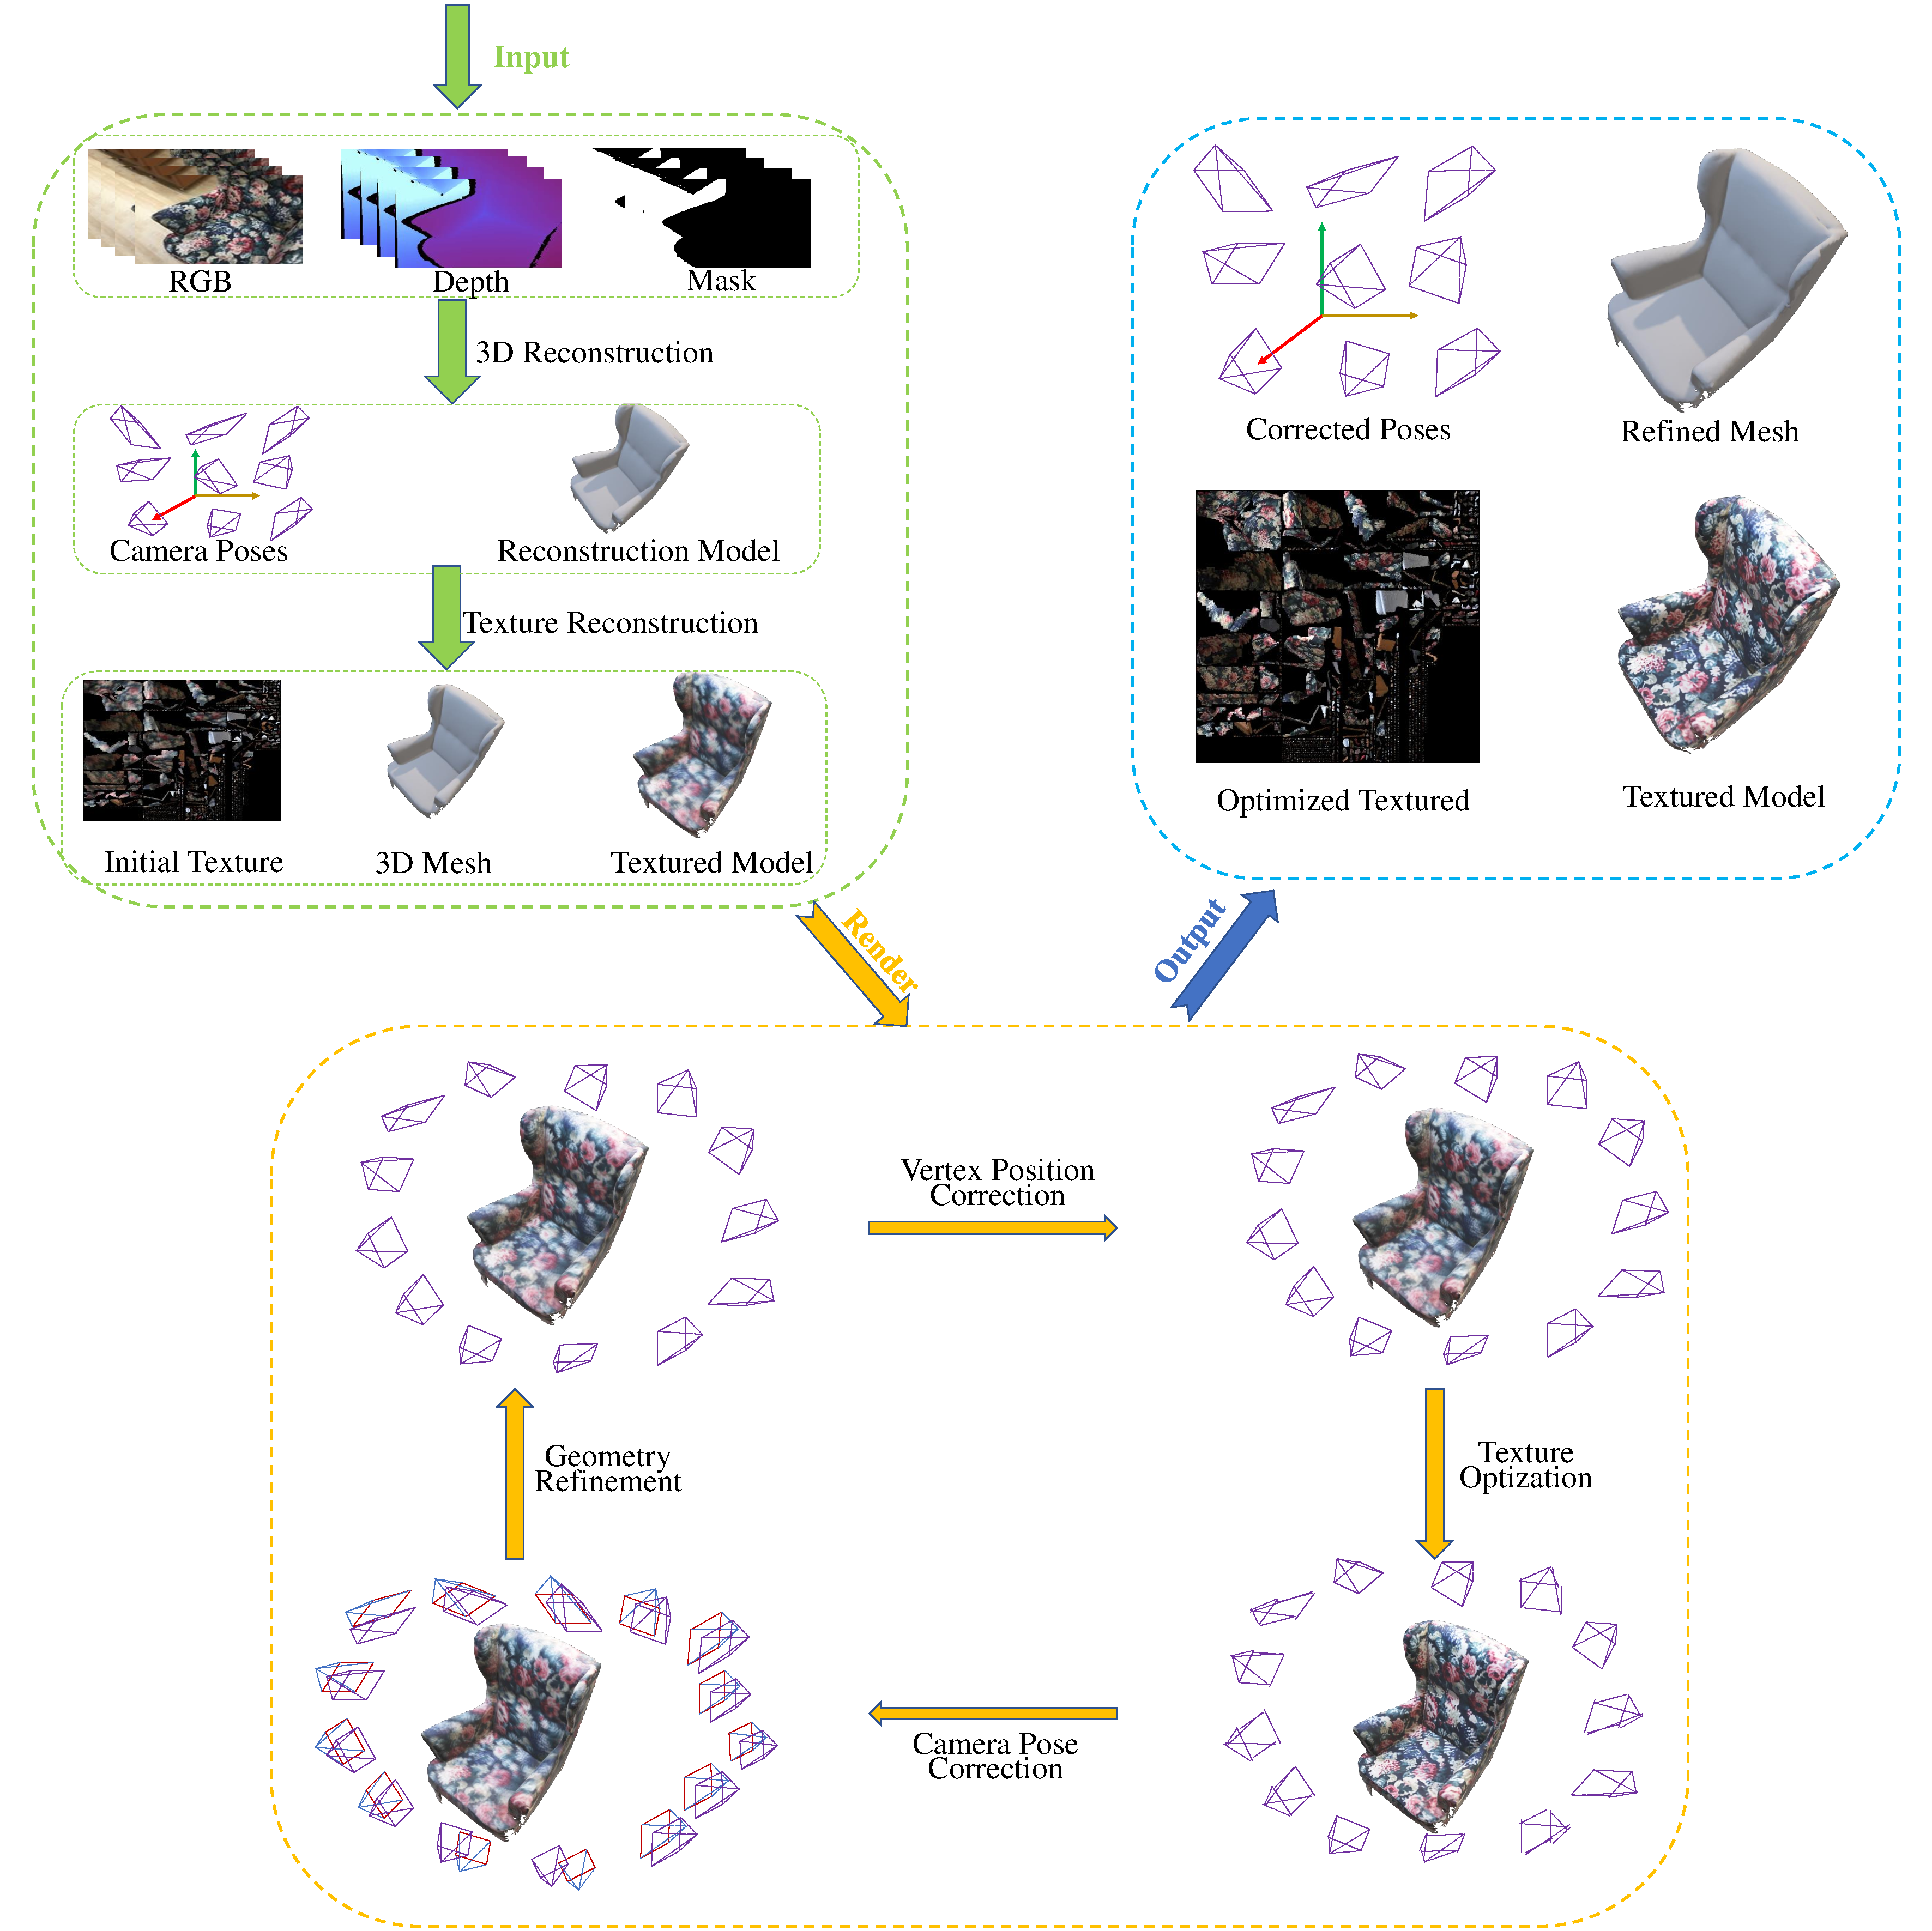
\includegraphics[width=1\columnwidth]{pic/work2/work2.pdf}
    \bicaption{基于可微分渲染的联合优化概述}{The overview of Joint optimization  based on differentiable rendering} 
    \label{fig:work2}
\end{figure}

本文提出的方法旨在利用RGB-D相机获取带有精细几何细节和高保真纹理贴图的三维模型,并通过联合优化算法实现此目标。具体而言,本文通过优化几何模型、纹理图像和相机位姿来实现其重建。优化几何模型可以恢复模型中高频的几何细节,而优化纹理则可以重新生成高保真度的纹理,并通过优化相机位姿来矫正估计不准确的相机位姿。图~\ref{fig:work2}展示了本文算法的完整流程。算法输入包括彩色图像、深度图像和掩码图像,通过三维重建产生初始的三维模型和每个图像对应的相机位姿。然后,利用纹理重建算法生成初始的纹理图像,但由于各种误差存在,初始纹理通常比较模糊。接下来,借助可微分渲染技术,本文矫正相机位姿的不精确性,并利用自适应细分方法在模型中增加几何细节,以及更新其位置以矫正几何误差,最后利用对抗生成网络重合成纹理图像。经过多次迭代优化,最终可以得到具有高频几何细节和优化后的纹理图像的三维模型。\par

在这个部分,本文将详细阐述本文提出方法的具体步骤。本文采用$P$表示纹理图,$M$表示初始几何模型(采用网格表示),$T$表示相机外参,$K$表示相机内参。其中,$I_c$、$I_D$和$I_S$分别表示手持RGB-D相机拍摄的彩色图、纹理图以及采用标准计算机图形学管线生成的掩码图。纹理、几何模型和相机位姿是本文目标恢复清晰保真纹理的关键,且三者之间耦合性极高。值得注意的是,渲染本身就需要纹理、相机和几何模型的共同参与,这与本文的优化目标高度契合。借助pytorch3d\upcite{ravi2020pytorch3d}可微分渲染框架,本文可以依据其渲染流程制定更加合理的优化策略,即分别对每个部分进行交替迭代优化而非采用多变量共同优化的混合策略,可以使得纹理、相机位姿和网格的优化过程相对独立,但是又高度内聚。下一个章节中,本文将详细介绍在优化框架中,纹理、相机位姿和网格的各自优化过程。\par


\subsection{数据预处理}
本文的算法可以是深度相机采集的原始数据,但是为了保证输入数据的规范性以及符合优化算法的输入,原始数据还需经过预处理,本文仍旧采用第三章第四节所述预处理方法。由于在网格重建后往往会有重复顶点,三角形面片可能会自相交,不符合网格的2D拓扑流形结构,在移动顶点位置后会发生显而易见的的裂缝。此外,由于在重建过程遮挡,噪声干扰等因素使得重建模型存在明显的孔洞。为了防止优化过程出现异常情况,如裂缝现象。本文先用meshlab\upcite{LocalChapterEvents:ItalChap:ItalianChapConf2008:129-136}剔除重复顶点和面片以及零面积面片,以保证几何模型的规范性。


\subsection{相机参数优化}
在基于RGB-D的三维重建中,通常使用光束平差法\upcite{BA}估计初始的相机位姿,然而估计结果只能保证相对准确,使用不完美的相机位姿渲染图像会导致渲染图像和采集图像错位。为了解决这个问题,本文利用可微分渲染框架对相机位姿进行矫正。在第三章中介绍的相机优化方法的基础上,本文额外增加了一个变形场$F$,用于矫正相机内参。为每个图像添加一个非刚性的优化过程,以矫正因不精确的几何和光学畸变而导致的复杂扭曲。设图像平面$I_i$上一点$\mathbf{u}$,定义在图像$I_i$上的变形函数$F_i$,$f_{i,l}$为二维向量。则变形函数定义为:
\begin{equation}
	\mathbf{F}_{i}(\mathbf{u})=\mathbf{u}+\sum_{l} \theta_{l}(\mathbf{u}) \mathbf{f}_{i, l}
\end{equation}
其中,$\theta_{l}(\mathbf{u})$为双线性插值函数,考虑到在给投影顶点施加移动向量,投影位置会在像素点之间,所以本文应用双线性插值函数为投影选择最佳的合适位置。由于投影过程与矫正过程是可微的,相机内外参矫正可以有机地结合。\par
受三维重建算法\upcite{DejanAzinovic2021NeuralRS}启发,本文使用6层Relu\upcite{agarap2018deep}激活函数的多层感知机在像素空间内附加二维变形场,以考虑输入图像中可能的扭曲或相机固有参数的不准确性。本文实验研究后发现,在同一场景中,所有图像扭曲失真情况的原因相同,如可能来自于相机内参的不准确性。在矫正域每一帧共享多层感知机的参数。在优化过程中,相机光线首先使用在使相机位姿投影至图像平面上然后从变形场检索的2D向量,然后用重投影误差函数公式\eqref{pose},共同优化变形场和相机位姿。

\subsection{基于自适应细分的网格优化}
\begin{figure}[ht]
    \centering

    \includegraphics[width=1.0\columnwidth]{pic/work2/mesh.pdf}
    \bicaption{基于可微分渲染的几何模型优化概述}{Overview of geometric model optimization based on differentiable rendering}
    \label{fig:mesh}
\end{figure}


仅仅优化相机参数不足以保证网格上任意顶点投影至每个视角得到一致颜色,尤其是在网格重建误差较大情况下。此外,在重建三维模型时一般会选用加权平均方法来抵抗重建过程中的噪声,虽然这种方法卓有成效,但是会造成过平滑的效果致使网格失去几何高频细节。本文同样也借助于可微分渲染方法恢复出几何表面的高频几何细节。本文为网格上每个顶点施加偏移量来矫正几何误差。\par
仅仅只更新顶点位置不足以保证几何模型细节突出,因为几何模型本身就过于平滑。本文采用质心细分网格方法增加三角形面片数目,一方面能使得模型更加契合真实世界场景,另一方面能减小顶点优化时发生漂移现象。即使如此,细分网格代价是巨大的,增加顶点面片数目会线性增加渲染时间,并且在一些含有平面较多且纹理单一的几何模型上细分视觉效果并不明显。本文实验中发现优化几何模型时,顶点移动频繁发生在纹理丰富的地方,而纹理较为单一时顶点移动并不明显。因此本文建议根据场景本身的纹理丰富程度来决定是否要细分以及细分的程度。如图~\ref{fig:subdivion}所示网格自适应细分流程。具体地,本文遵循以下步骤:
\begin{enumerate}[label=(\arabic*),leftmargin=\parindent,align=left,labelwidth=\parindent,labelsep=0pt]
	\item 用soble算子提取所有视角的梯度图$\nabla g_i$,作为细分面片的依据。
	\item 计算几何模型上每个面片$f_j$投影至每个可见视口$i$的面积$A_{ij}$,并求出面积总和$\sum_{i}^{n} A_{ij}$。
	\item 计算每个面片$f_j$采样概率$\sum_{i}^{n} A_{j} / \sum_{j}^{m}\sum_{i}^{n} A_{ij}$,其中m为几何模型中面片数量,n为视角数量。
	\item 按照概率对所有面片进行无放回随机抽样,并设定采样概率阈值为0.5,在阈值概率之上面片才会被选取。
	\item 对所选择面片$f_j$进行质心细分。
\end{enumerate}

\begin{figure}[ht]
    \centering
%  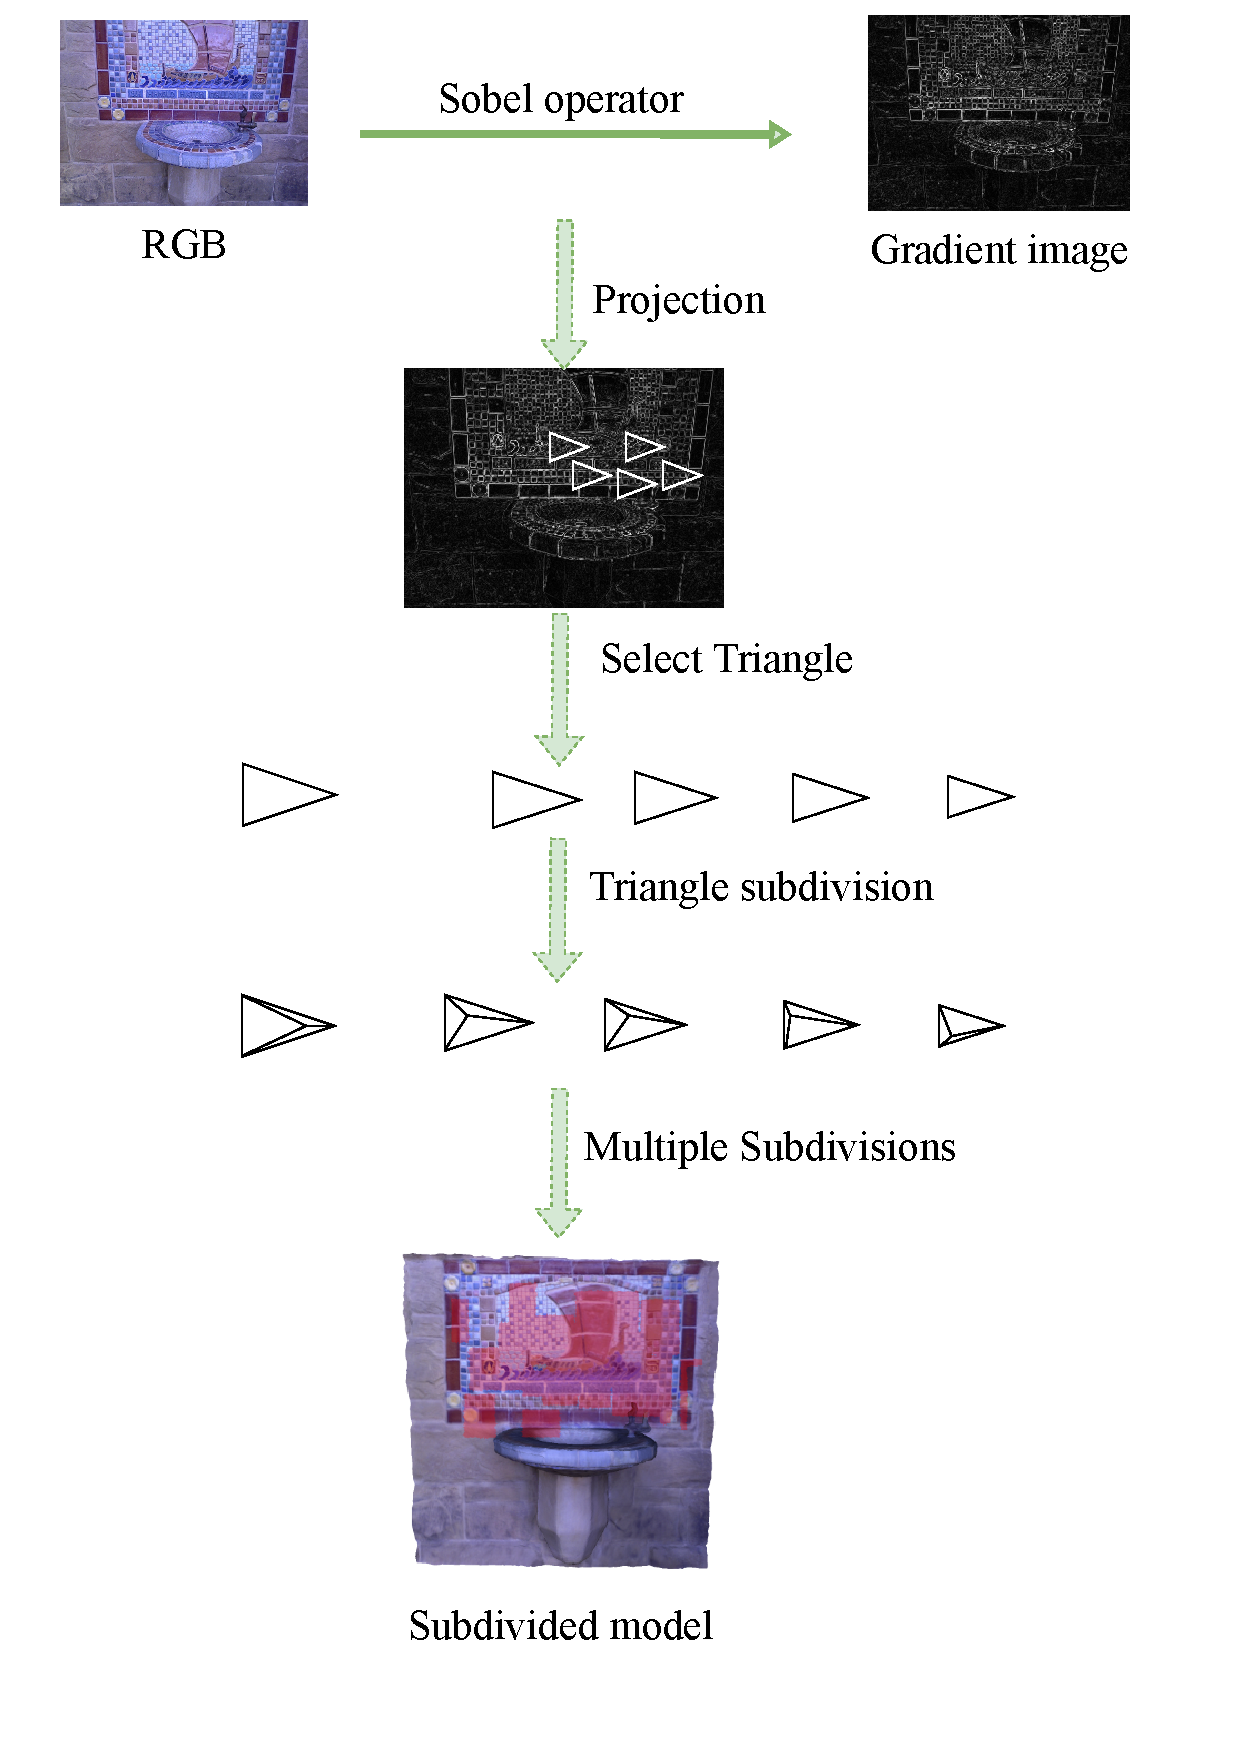
\includegraphics[height=0.5\textheight,keepaspectratio]{pic/work2/Mesh_subdiv.pdf}
    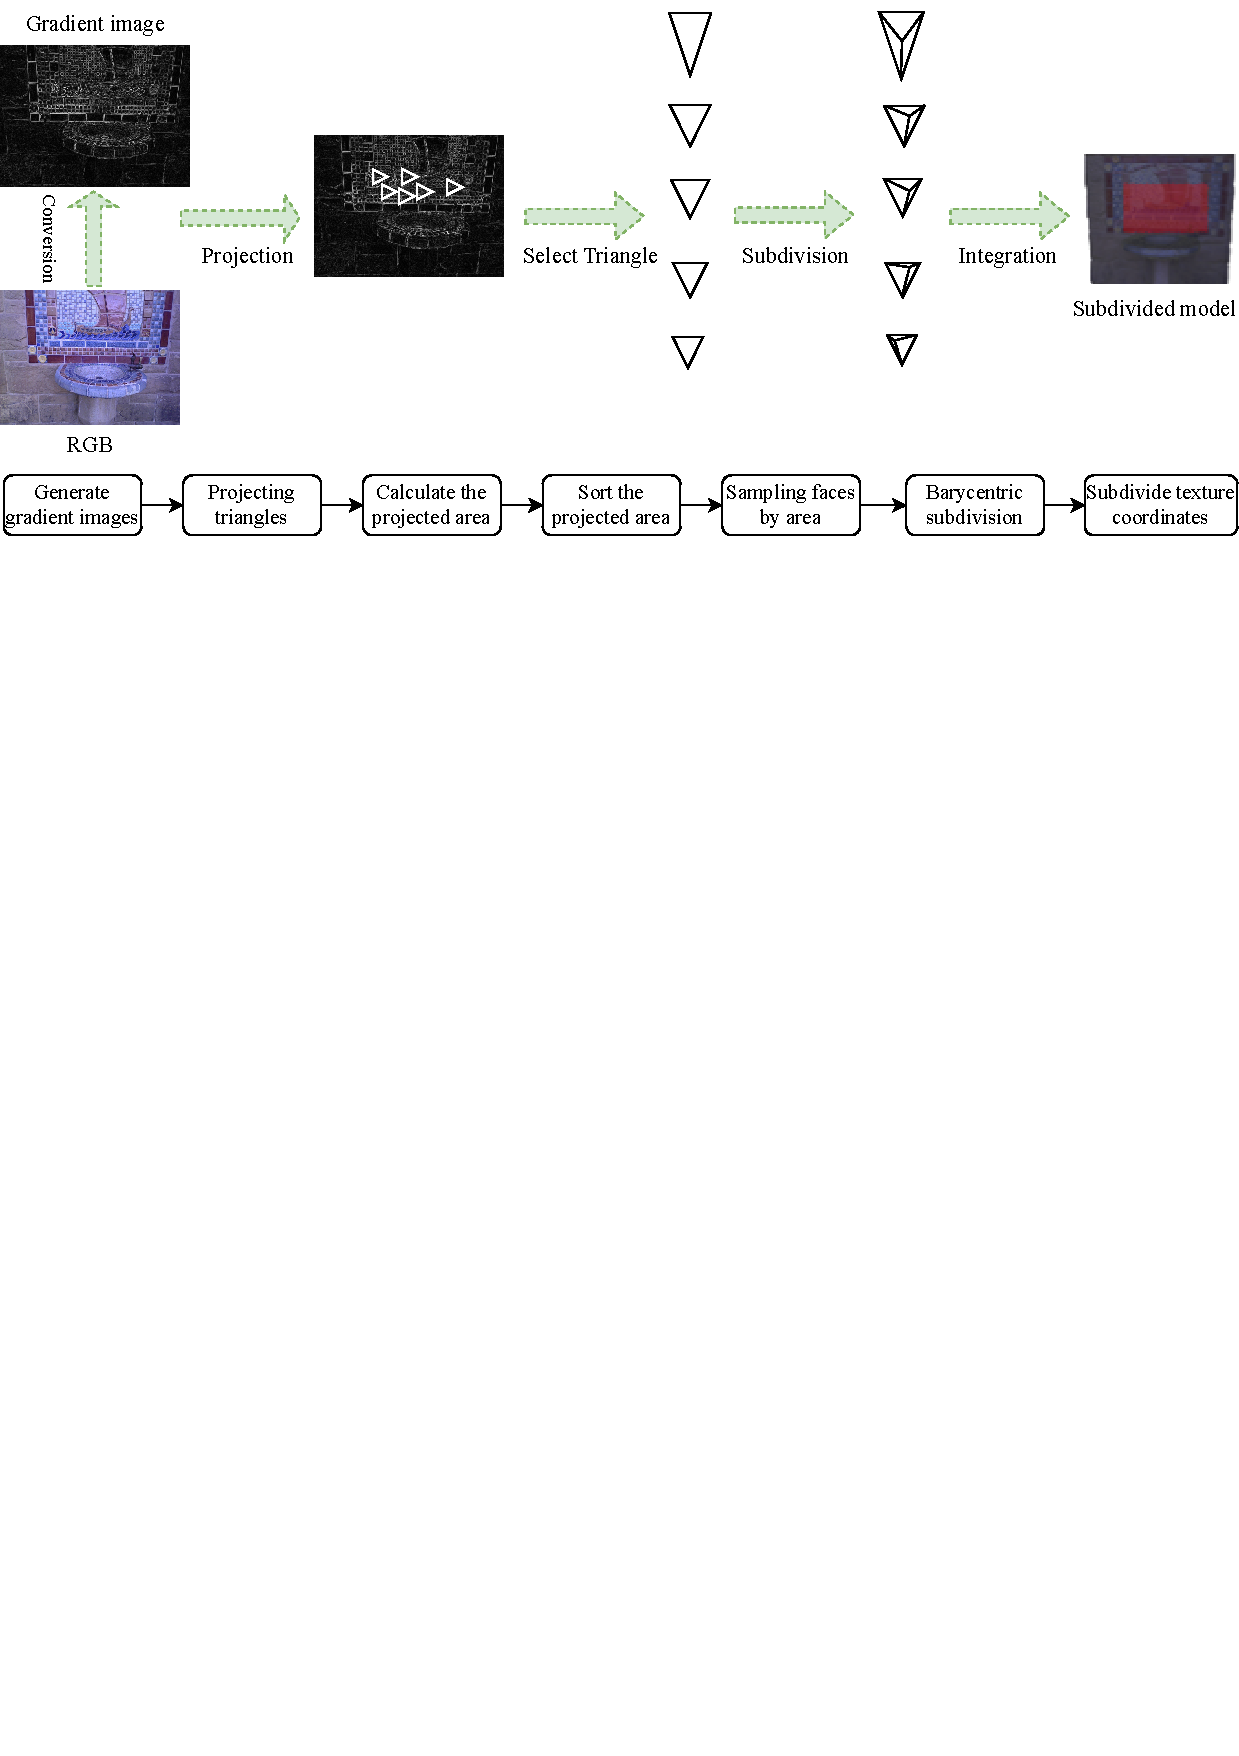
\includegraphics[width=1.0\columnwidth]{pic/work2/mesh_subdivision.pdf}

    
    \bicaption{网格自适应细分概述}{Overview of Adaptive Mesh subdivision }
    \label{fig:subdivion}
\end{figure}

本文在第四步随机抽样时,为了防止太多的面片不在查询集合中,本文使用中位数而不是平均值作为采样阈值。细分完成后,本文仍用同样的方式增加对应的纹理坐标,以保持顶点和纹理坐标的对应关系。\par
优化几何模型时仅仅有图像间损失是远远不够的,因为每次迭代中顶点移动不受约束,会破坏网格模型的拓扑结构,导致三角形退化。因此本文在图像损失基础上增加了几何正则化项,即拉普拉斯项、法线一致性项和$L2$ 范数。\par
拉普拉斯项定义为顶点坐标减去其临近顶点的加权和,在优化过程中可以保持局部几何特征不变。在优化过程中,拉普拉斯损失项可以帮助模型收敛到一个更加平滑的解,从而提高几何模型优化的准确度和稳定性。它也可以有效抑制因噪声或不规则采样而产生的噪点,使得优化结果更加符合实际。令$V \in \mathbb{R}^{n\times3}$为存储顶点位置的矩阵,则拉普拉斯项定义为:
\begin{equation}
	E_l = \sum_{i=1}^{n}\left \| LV \right \|_2 
\end{equation}
其中,$L\in\mathbb{R}^{n\times n} $是网格的拉普拉斯图。\par
在优化过程中为了防止顶点偏移初始位置太远,本文用$L_2$正则化项来约束顶点偏移量。其中$\mathbf{v}_{i}$为初始网格的顶点坐标,$\widetilde{\mathbf{v}}_{i}$为当前网格顶点的坐标。
\begin{equation}
	E_{r}=\sum_{i}^{n}\left\|\mathbf{v}_{i}-\widetilde{\mathbf{v}}_{i}\right\|^{2}
\end{equation}

最后,为了保证网格具有平滑性,本文额外使用了网格法线一致性损失。即利用余弦相似度计算相邻面片的法线一致性。
\begin{equation}
	E_n= \frac{1}{|\overline{\mathcal{F}}|} \sum_{(i, j) \in \overline{\mathcal{F}}}\left(1-\mathbf{n}_{i} \cdot \mathbf{n}_{j}\right)^{2}
\end{equation}
其中,$\overline{\mathcal{F}}$代表共享一条边的相邻三角形面片的集合。$i$,$j$表示任意一对儿三角形面片。\par
最终网格重建损失项表示如下:
\begin{equation}
	L_M = L_T + \lambda_l E_l +\lambda_r E_r+\lambda_n E_n
\end{equation}
在实际优化中,本文分别设置$\lambda_l = 1000$,$\lambda_r = 1000$,$\lambda_n = 10$。\par

详细更新流程如图~\ref{fig:mesh}所示,对于重建模型本文首先进行自适应细分策略,然后经过可微分的光栅化阶段,从Zbuff中获取深度图和掩码图像。然后本文用布林冯着色模型\upcite{blinn1977models}对投影像素着色得到渲染图像,最后损失项回传梯度,更新网格顶点位置。

\subsection{纹理重合成}
仅仅只矫正相机位姿和网格顶点位置是不够的,优化结果并不能完全消除噪声。况且本文采用顶点加权融合方式生成纹理,仍存在模糊并且缺失细节。对于残留的微小位姿误差、几何误差、光源干扰等再使用优化算法收效甚微。受纹理图像合成法\upcite{bi2017patch,JingweiHuang2020AdversarialTO}的影响,本文利用图像合成法合成新的纹理图。具体算法与第三章所著的纹理合成模型相同。本文在此基础上额外添加了频域空间损失以保证纹理合成不会出现模糊失真。\par

在生成对抗网络中尽管合成图像已经足够逼真,但是真实图像和生成图像在空间域中仍旧存在不易察觉的差距。将图像变换至频域后,这种差距变得尤为明显。基于这种发现,Jiang等人\upcite{jiang2021focal}提出新的频域损失,减少图像间的频域差距。本文由此得到启发,在对抗生成网络中加入频域损失函数。它可以自适应的关注深度生成模型难以合成的频率分量,纠正对神经网络存在的偏差性。从而提升模型在图像空间域合成的微小细节的能力。文本在公式\eqref{texture}基础上本文额外添加了Focal Loss损失:
\begin{equation}
	L_\mathrm{FFL}=\frac{1}{M N} \sum_{u=0}^{M-1} \sum_{v=0}^{N-1} w(u, v)\left|F_{r}(u,v)-F_{f}(u, v)\right|^{2}
\end{equation}
其中,$M,N$为图像宽高,$w(u,v)$为图像$(u,v)$位置处的频域分量权重。\par
经过若干次迭代交替训练判别器$D$和纹理$P$后,神经网络会学习三维场景中存在的各种误差,并在生成容忍这些误差的清晰的纹理图像,而不需要额外更新已有的纹理映射关系。 与加权融合方法生成的纹理相比,优化后的纹理更逼真,更接近真实彩色图像。\par

\subsection{交替优化}
相似于之前工作\upcite{YanpingFu2020JointTA},本文使用联合优化策略优化相机参数、几何模型和纹理。本文用相机-几何模型-纹理优化顺序进行。一方面是在相机和网格优化中纹理生成方法不同于对抗神经网络的像素重生成方法,另一方面在矫正相机参数和网格后,对抗生成网络效果重生成的纹理更加贴近于真实世界场景。具体地,本文采用外部循环方法分别优化参数集合$(T,M,P)$。本文首先固定参数$(M,P)$,通过最小化损失函数$L_T$以优化每一帧的相机参数$T$至$T'$;其次,本文使用参数$(T',P)$最小化损失函数$L_M$优化几何模型$M$至$M'$;最后本文使用并固定前两次的结果参数$(T',M')$最小化对抗损失$L_{adv}$来优化纹理$P$至$P'$。\par
在时间和效率的权衡下本文重复外循环优化策略3次。并且本文遵从由粗到细的策略优化不同的目标。具体地,在每一次外部迭代$t\in \left \{ 1,2,3 \right \}$中本文用指数衰减方式控制内部迭代次数,即内部迭代次数为$\text{epoch}  =\frac{s}{2^{t-1}}$,其中s为每一个内部迭代初始的轮数。此外,学习率也会相应地进行调整。实验研究发现,利用指数衰减策略,可以保证最终效果的同时显著减少优化时间。本文设置初始的优化相机参数、优化几何模型和纹理次数分别为50,50,100。

\section{实验结果与讨论}
在本节中,本文在各种不同的真实场景下进行定性分析,以证明所述方法的有效性。本文与最近提出的纹理优化方案G2Tex\upcite{fu2018texture},JointTG\upcite{YanpingFu2020JointTA}和ATO\upcite{JingweiHuang2020AdversarialTO}进行比较。其中G2Tex为基于面的投影方案生成的场景纹理,面纹理直接来自于投影图像,最终生成的纹理清晰度与拍摄照片一致。这种方案旨在解决相邻面片纹理间的错位现象。ATO、JointTG与本文提出的方法,主要以顶点颜色加权融合生成物体纹理,虽然不会发生纹理图像的错位,但是容易产生模糊伪影等问题。不同的是ATO采用生成对抗网络重新生成新的高清纹理图像,作为纹理映射结果。JointTG通过联合优化方法,同时优化纹理、网格和相机位姿抵抗重建模型过程中的噪声以获取最清晰的纹理。对于另一个联合优化方案Intrinsic3D\upcite{RobertMaier2017Intrinsic3DH3},因为Intrinsic3D在优化过程中,采用细分体素方案生成密集网格作为算法的结果,不需要在算法输入时候提供网格模型。而本文数据集提供了初始的网格模型,为了标准统一,所以不再进行实验对比。
在实验中,使用各个方法发布的源代码进行比较。由于G2Tex与JointTG作者在论文中说明需要选择关键帧作为算法的输入。在某些没有发布关键帧序列的场景下,如椅子数据集\emph{Chairs},本文按照清晰度度量指标选出若干张覆盖物体全景且最清晰的图像为关键帧,作为G2Tex与JointTG算法的输入。最后,本文用消融学习策略证明本文所提出的算法的有效性。本文的实验环境与评估指标等其它实验设置均和第三章所描述的保持一致。


\subsection{公共数据集上结果与分析}
\begin{figure}[!t]
\centering
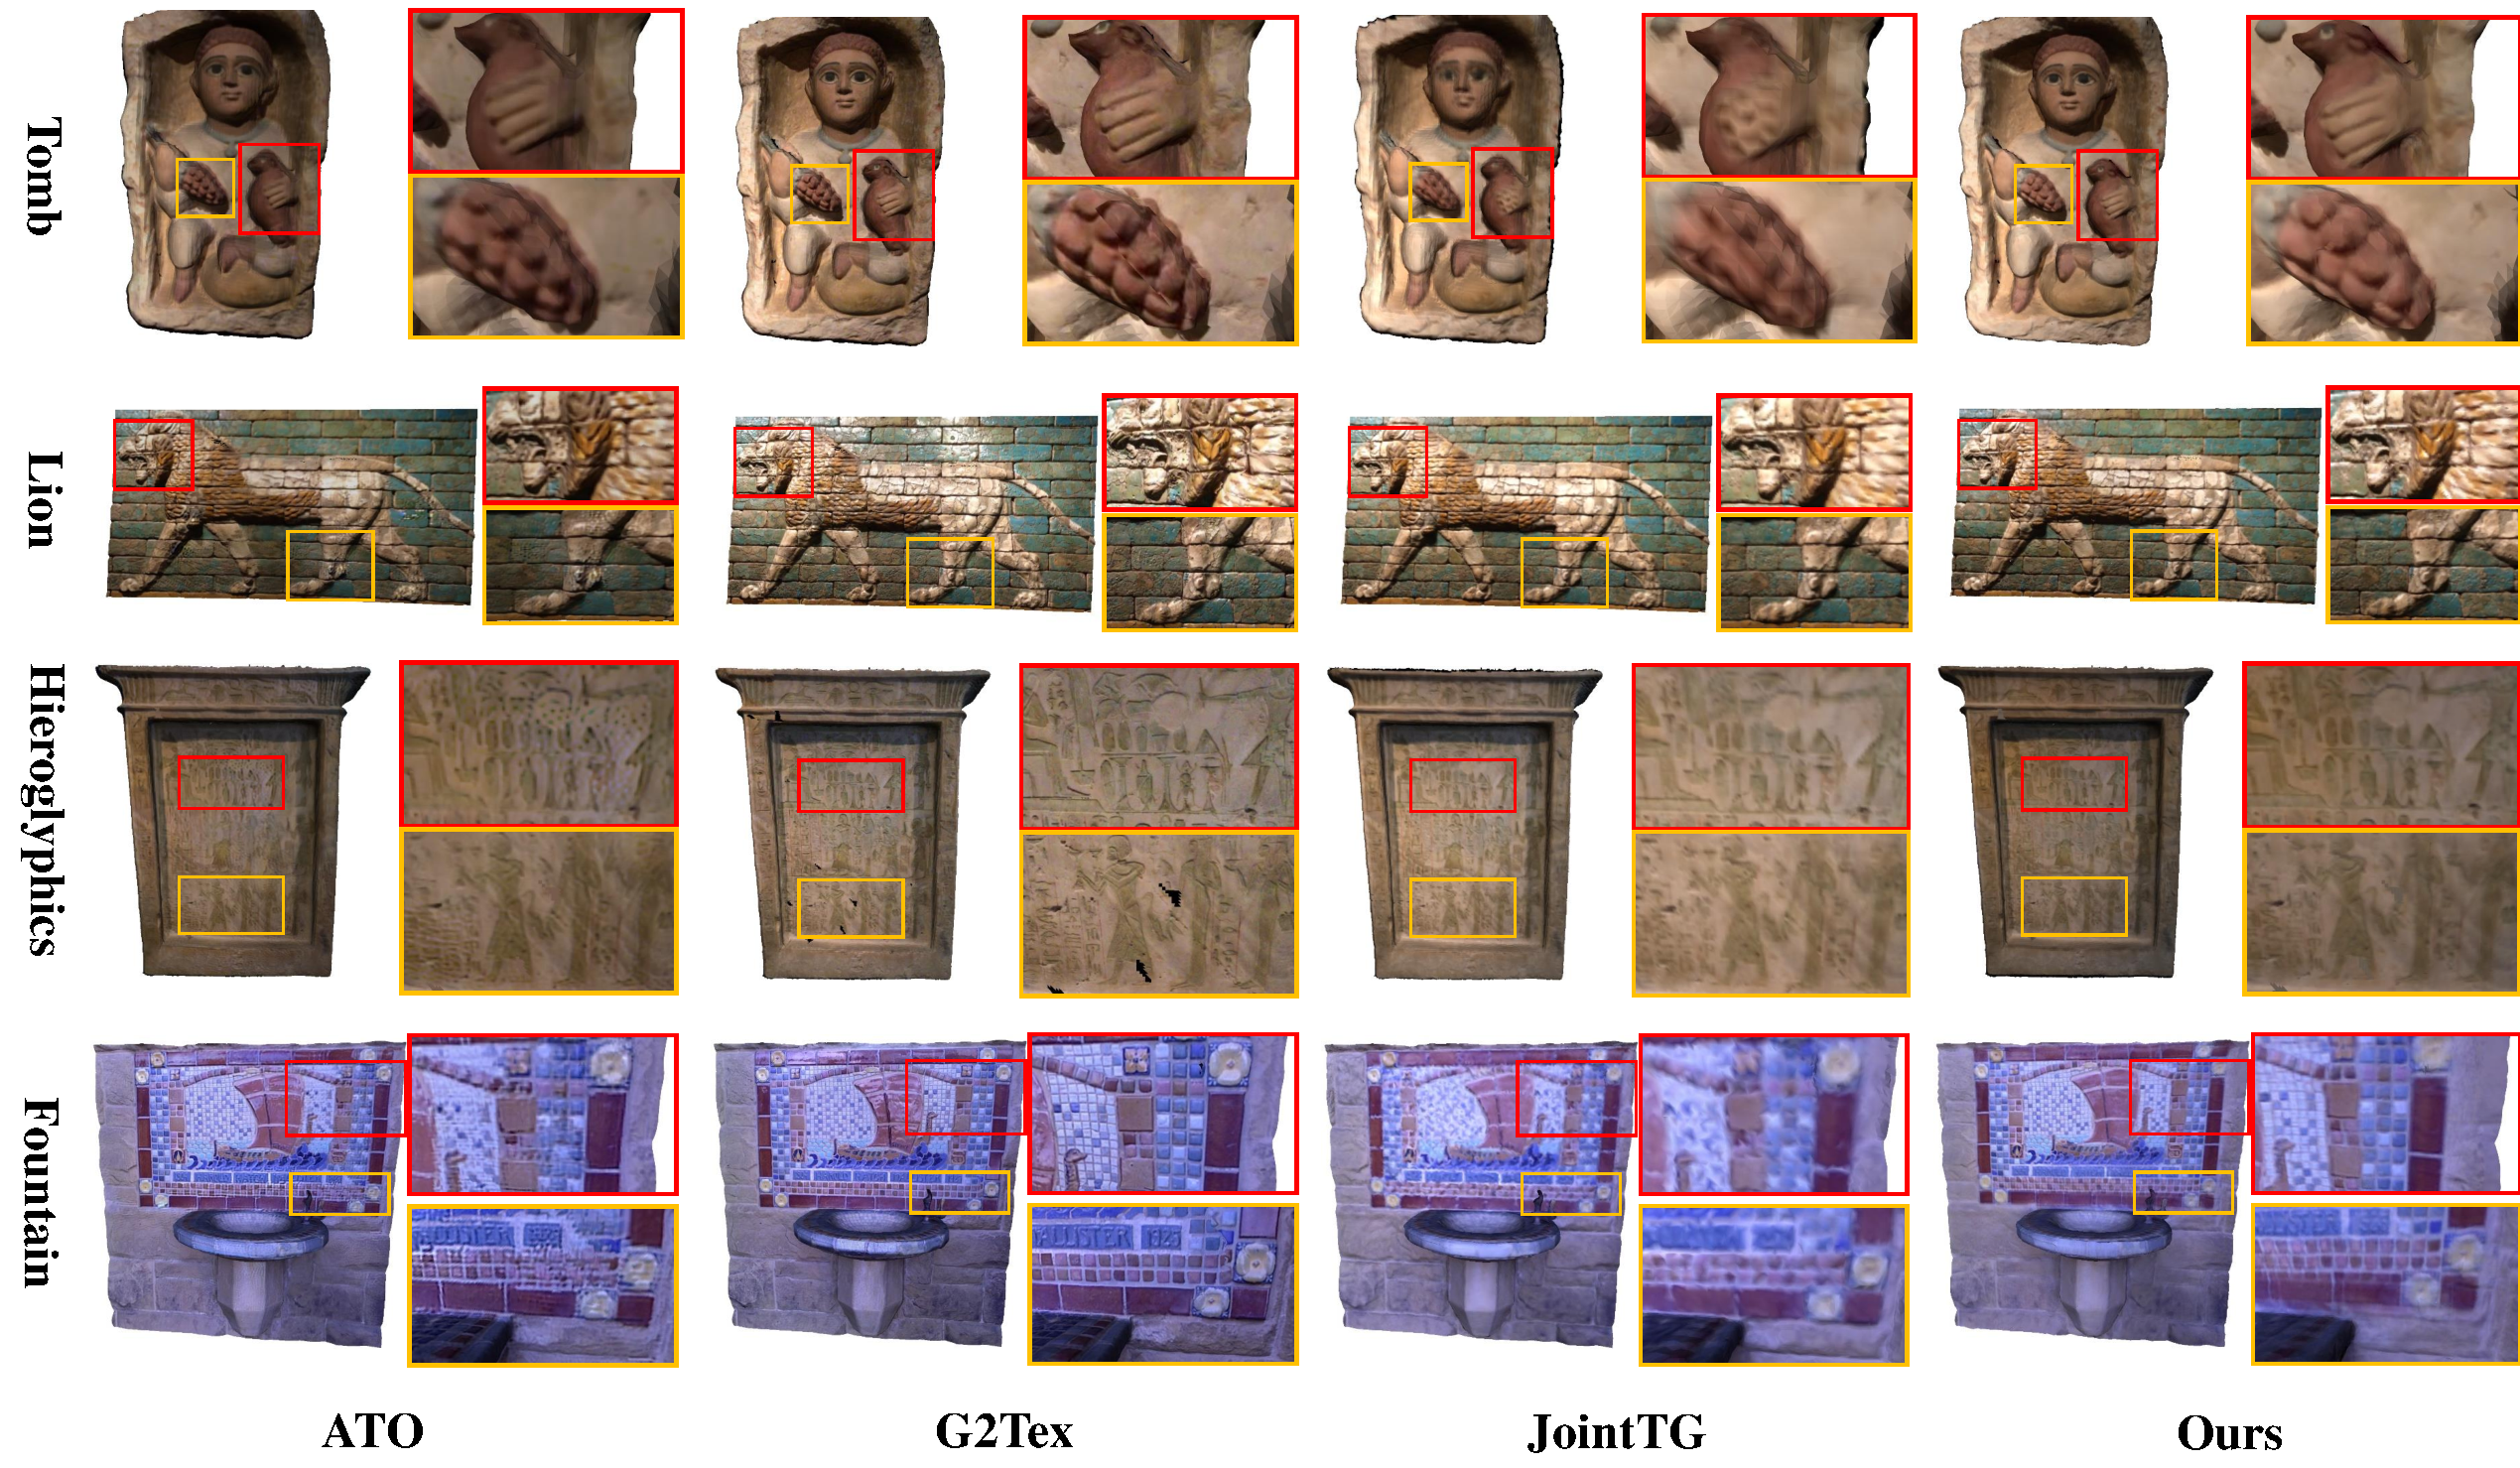
\includegraphics[width=1\linewidth]{pic/work2/compare3.pdf}
\bicaption{公共数据集上不同渲染方法的视觉比较 1}{Visual comparison of different rendering methods on public datasets 1}

\label{fig:ex2_3}
\end{figure}

本文首先在Intrinsic3D发布的公共数据集上进行评估,初始网格模型来自于Intrinsic3D重建出的体素模型。为了便于使用本文用Marching cubes算法\upcite{lorensen1987marching}抽取出基本的三维网格。如图~\ref{fig:ex2_3}所示,图片第一二三行均来自此数据集。该数据集颜色较为单一,且平面场景较多,这为纹理优化带来挑战性。本文的方法可以获取全局一致的纹理效果,从数据集\emph{Tomb}(图片第一行)可以看出本文所提出方法比ATO与JointTG产生的纹理映射结果清晰,从图中红色框展示的鹰的眼睛以及橙色框中的玉米棒图案可以看出。ATO方法虽然能产生全局一致的纹理,但是在某细节出会出现伪影,如\emph{Lion}场景下橙色框所展示的狮子的脚部,\emph{Hieroglyphics}场景下红色框中的图案。由于在平面场景下细节不够丰富,使用生成对抗网络无法完全重建物体的纹理细节,即使能够容忍较小的相机误差和几何误差,但是在局部地方仍然有模糊现象。\emph{JointTG} 在实现场景纹理细节处表现并不完美,如\emph{Hieroglyphics}的图案,\emph{Tomb}中人物的手部等。场景中模型顶点较少,无法突显出场景的局部细节。从清晰度角度看,G2Tex的结果最佳,但是无法保证全局一致性。如图第一二行红色框所示,纹理图像有明显的断裂情况。\emph{Hieroglyphics}场景下会出现孔洞现象。最后,本文也在Zhou等人\upcite{Zhou2018}发布的\emph{Fountain}场景下比较基线方法,该数据集视角非常稀疏。在此数据集上,本文的方法仍然可以获得高保真度的纹理。虽然,G2Tex使用面投影方法能产生最佳纹理,但是在加权融合策略下,本文方法在细节和清晰度方面优于ATO与JointTG。\par

\begin{figure}[!t]
\centering
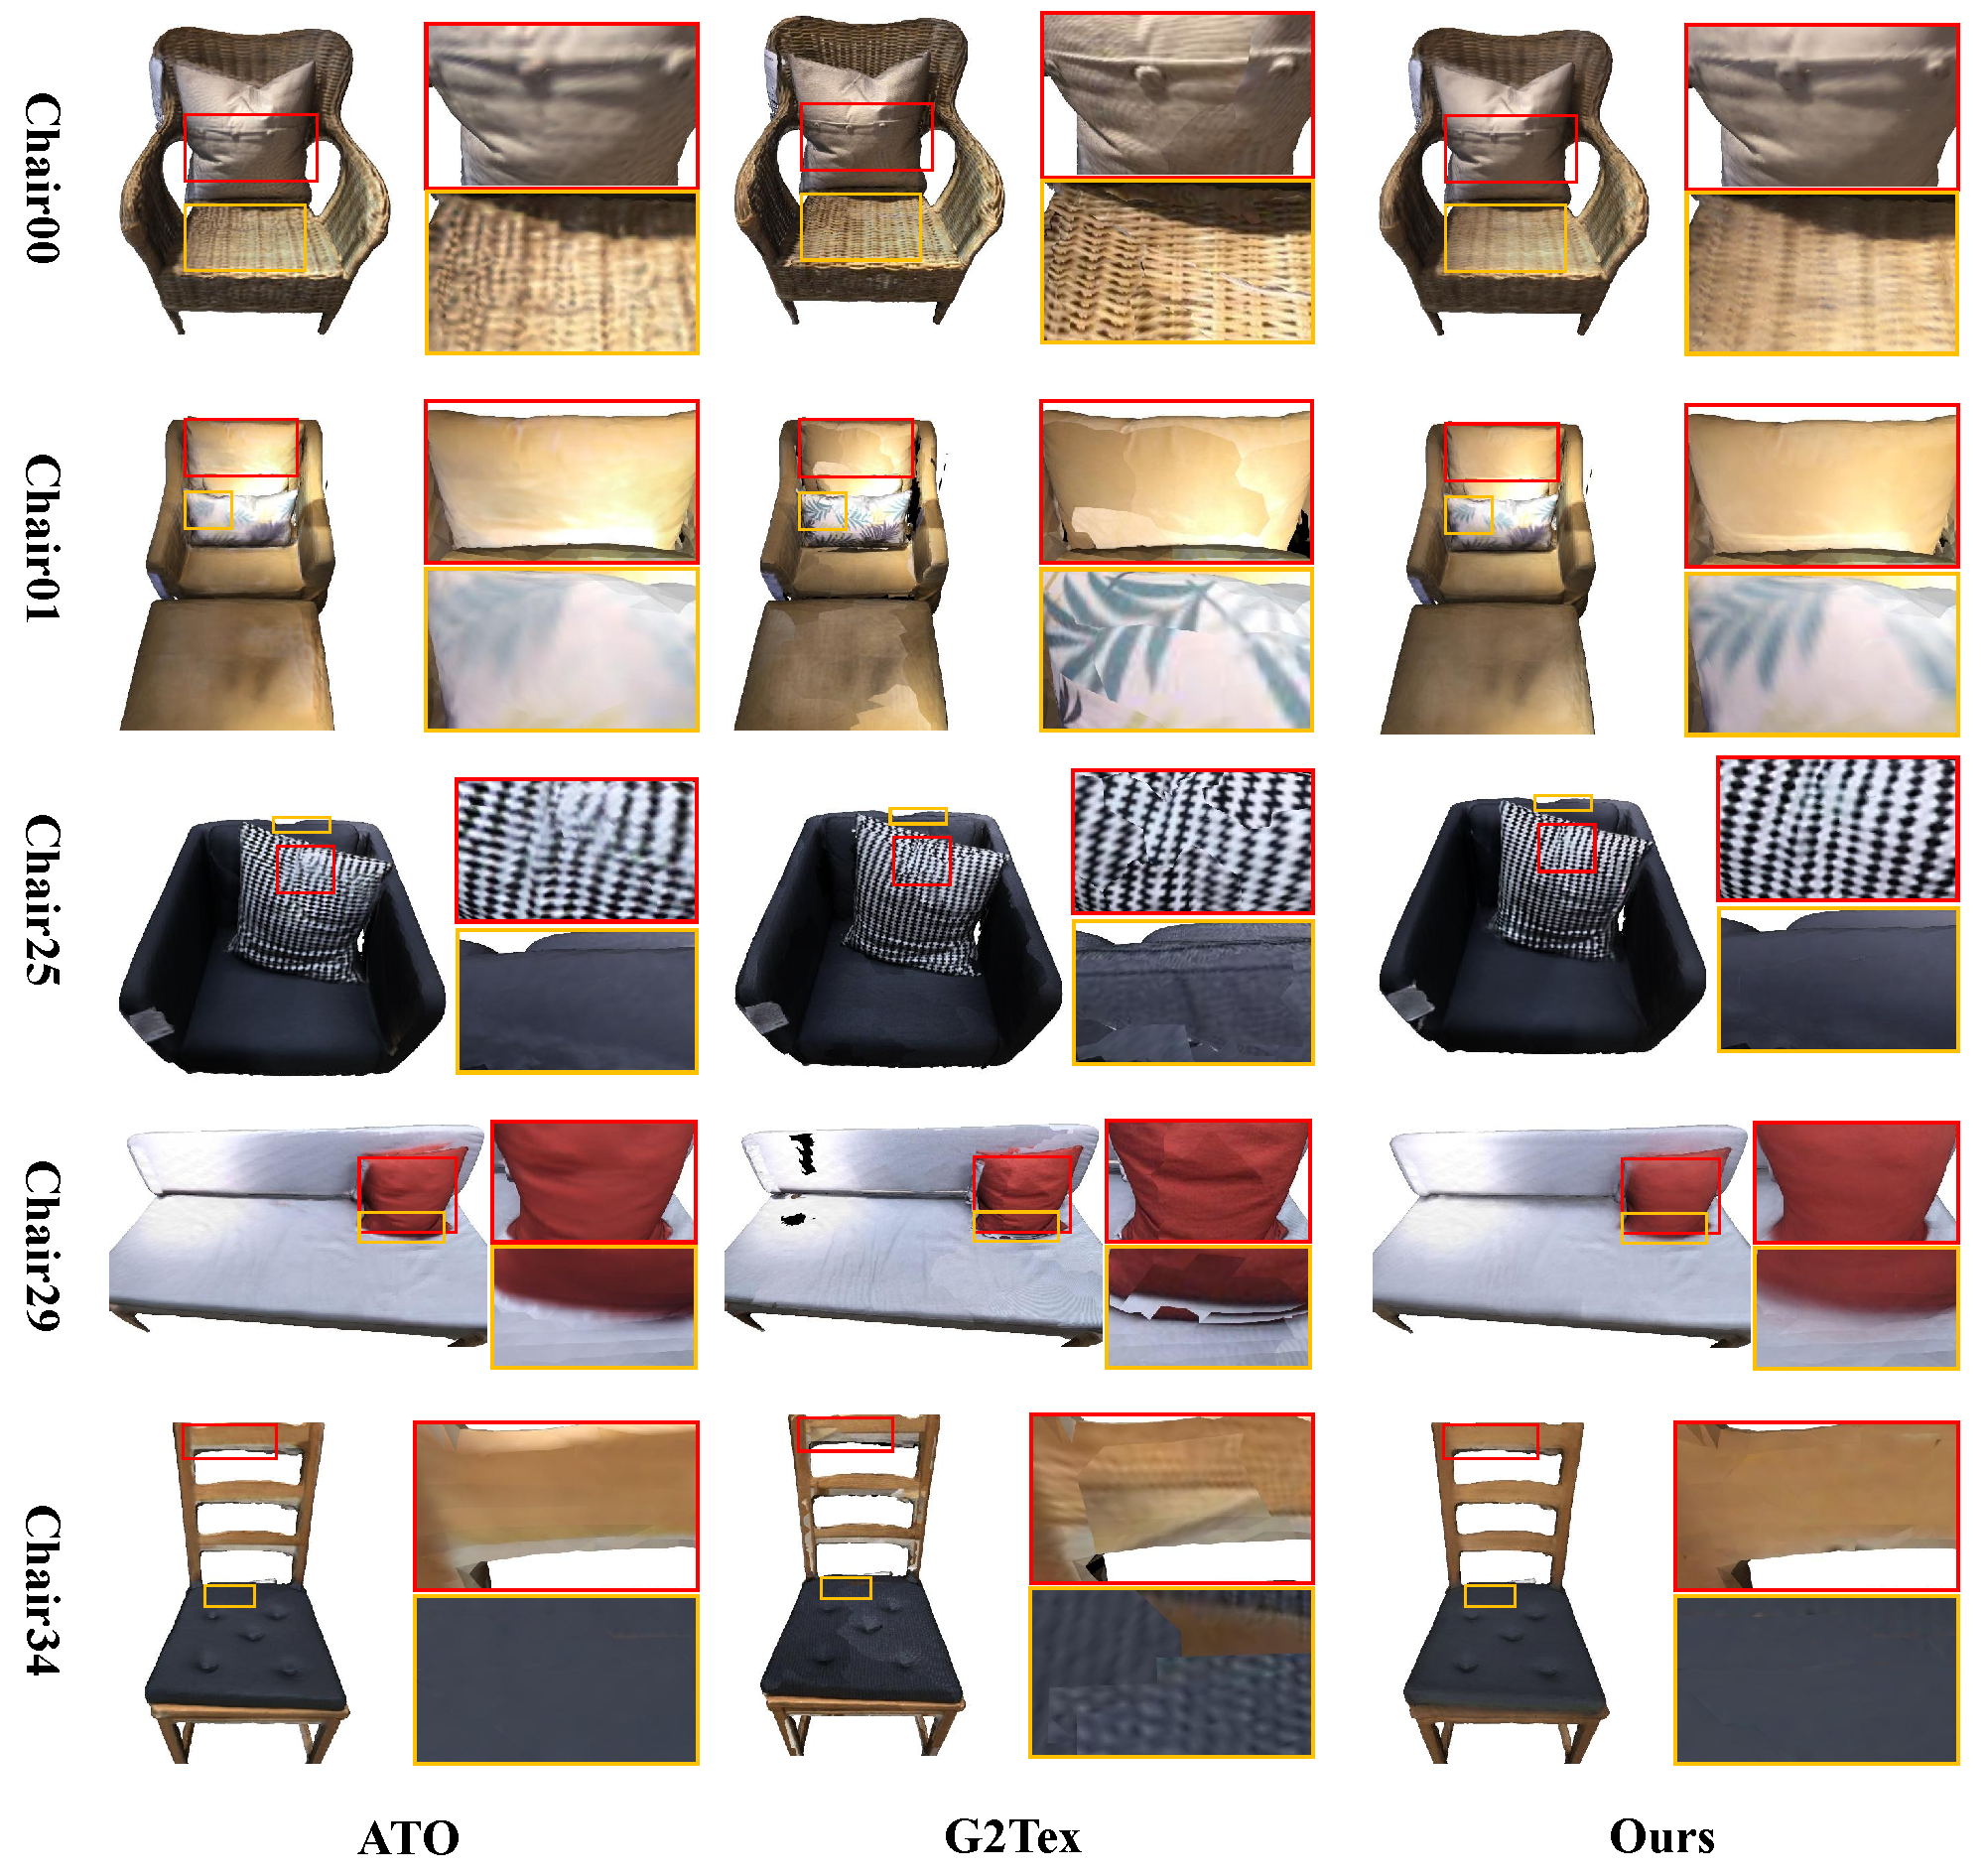
\includegraphics[width=1\linewidth]{pic/work2/compare1.pdf}
\bicaption{公共数据集上不同渲染方法的视觉比较 2}{Visual comparison of different rendering methods on public datasets 2}

\label{fig:ex2_1}
\end{figure}

本文在Chairs数据集同样做了对比,如图~\ref{fig:ex2_1}所示。该场景与Intrinsic3d数据集相比,纹理较为简单,给相机位姿矫正带来了挑战。由于该场景和模型顶点数量较少,JointTG利用顶点颜色表示物体表面外观的方法并不适用,所以本文不做比较。从图中所展示,本文与ATO均可得出全局一致的纹理,而G2Tex的全局矫正和局部扭曲纹理坐标方案并不能完全消除纹理裂缝。从图中\emph{Chair01}、\emph{Chair25}和\emph{chair29}场景下橙色框所展示,纹理图像间有明显的断裂。本文方法在颜色单一的场景下也能保持鲁棒性,而且从\emph{Chair01}场景的橙色框中可以看出,本文能够恢复出比ATO更丰富的纹理细节。\par

最后,本文在G2Tex发布的公共数据集上进行比较,如图~\ref{fig:ex2_2}所示。该场景使用kinect \emph{v}1深度相机拍摄。图像分辨率低,较为模糊,而且场景受灯光,几何噪声等因素干扰较明显。通过定性结果证明,本文的在恢复纹理外观细节方面优于ATO与JointTG。ATO通过融合来自多个视图的纹理信息和使用对抗网络来获得更好的纹理。尽管如此,它还是无法恢复微小细节,如\emph{Bolster1}场景。JointTG生成的纹理和网格在视觉上是和谐的,但是由于在优化网格过程中顶点发生移位使得平滑的表面变的粗糙,同时纹理也变得更加模糊。如\emph{Car}场景中橙色框,\emph{Desk}场景中红色框所示,本文能够获得全局一致的纹理外观。\par

\begin{figure}[!t]
\centering
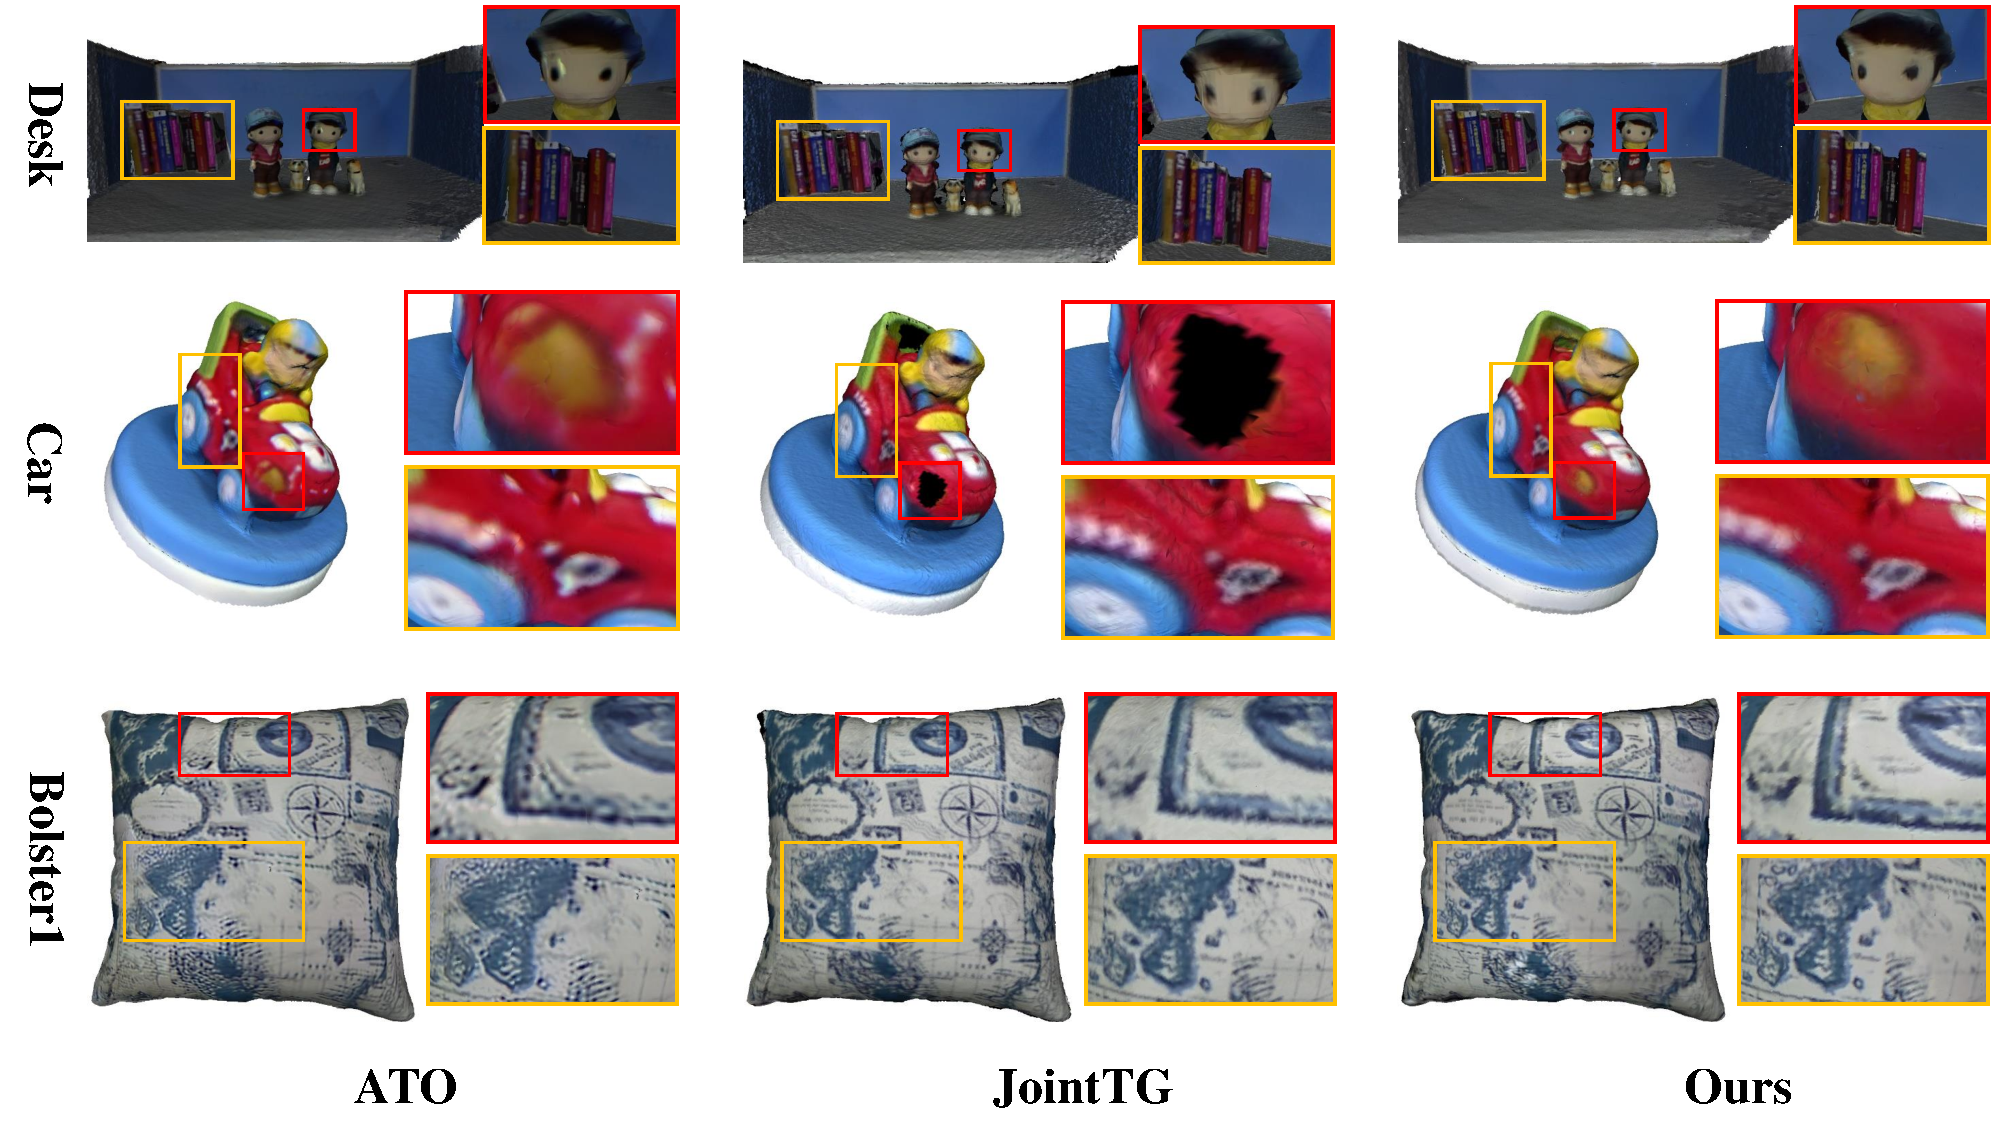
\includegraphics[width=1\linewidth]{pic/work2/compare2.pdf}
\bicaption{公共数据集上不同渲染方法的视觉比较 3}{Visual comparison of different rendering methods on public datasets 3}
\label{fig:ex2_2}
\end{figure}



\subsection{消融实验}
\begin{figure}[!t]
\centering
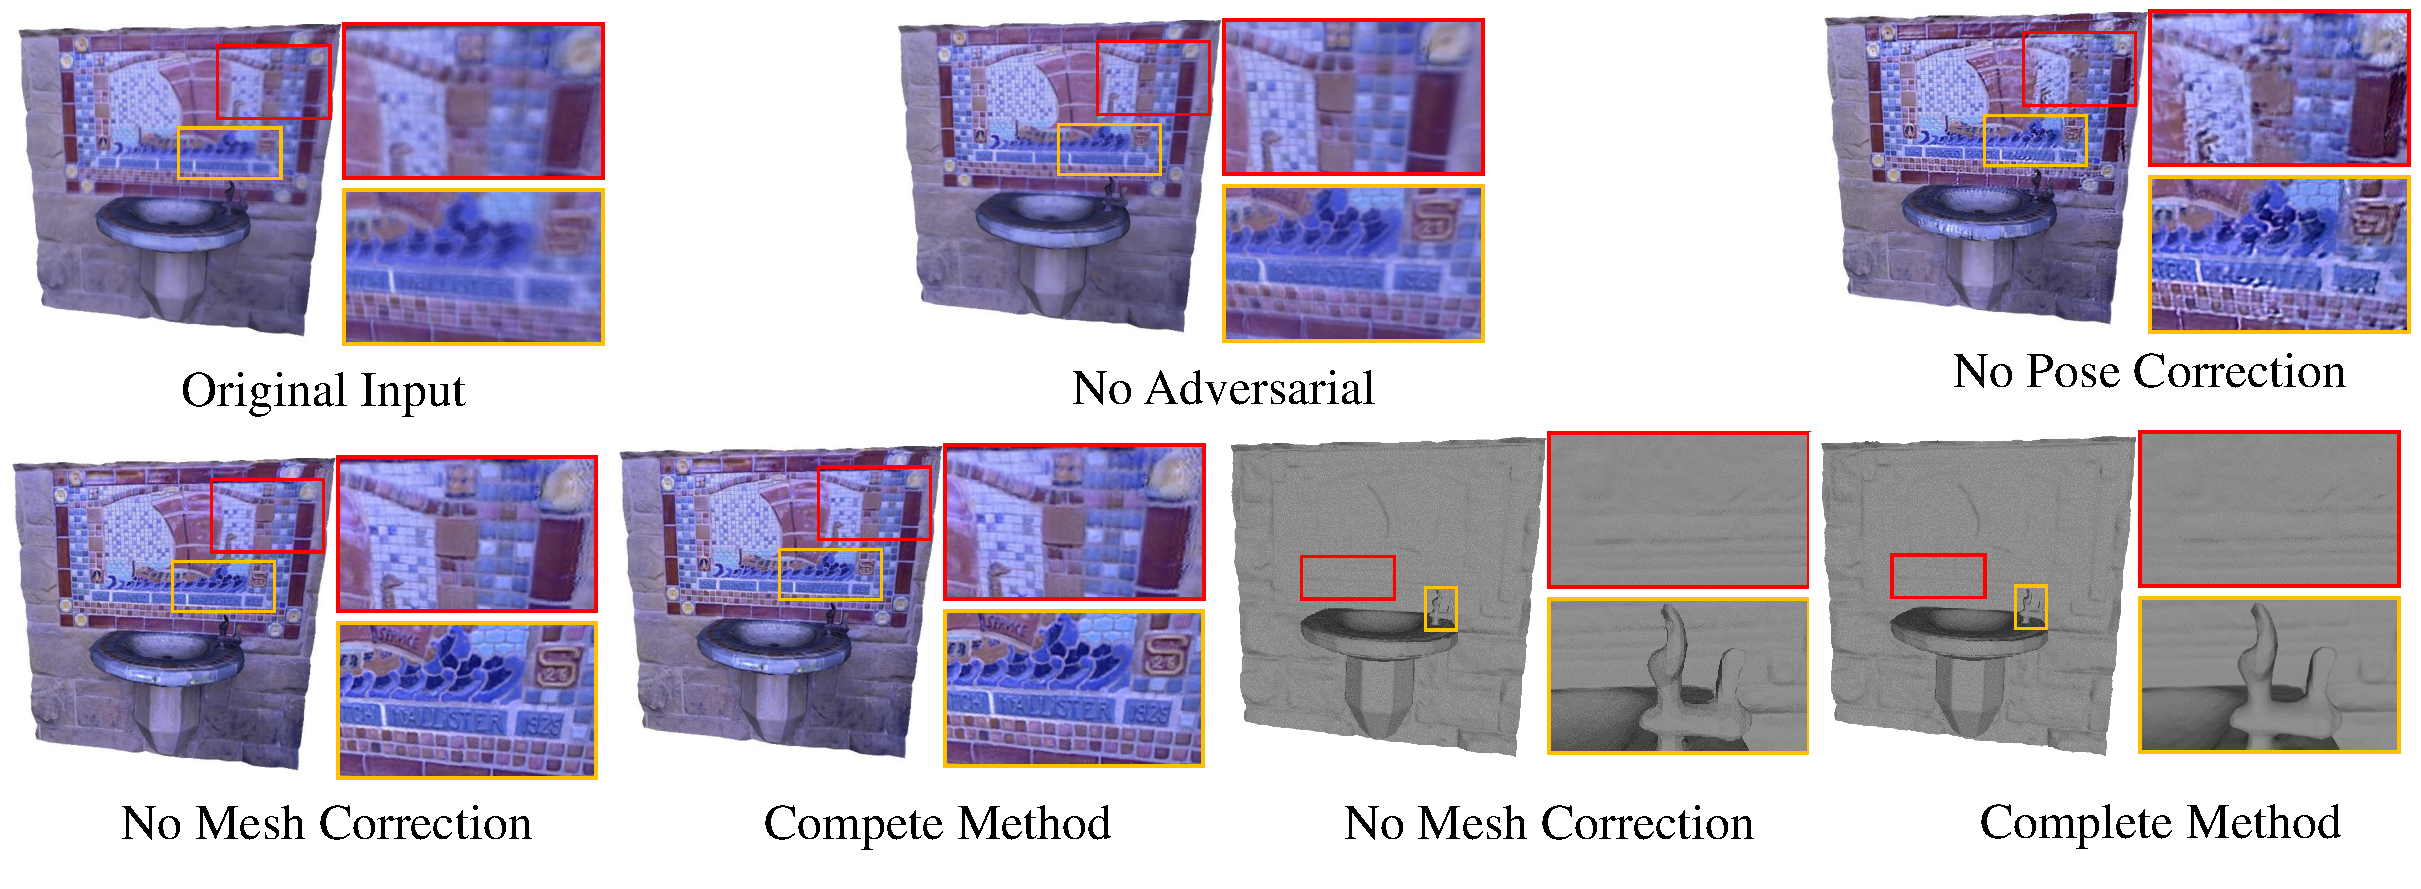
\includegraphics[width=1\linewidth]{pic/work2/compare4.pdf}
\bicaption{消融实验中纹理几何与相机位姿的定性比较}{Qualitative comparison of texture geometry and camera pose in ablation studies}

\label{fig:ex2_5}
\end{figure}





在这个部分,本文研究渲染框架中各个部分的有效性。为了更有说服力,本文选择公共数据集\emph{Fountain}。首先本文在没有矫正相机位姿,没有优化几何模型,没有对抗生成网络的情况下进行实验。最后,本文讨论自适应细分方法中基于面片的细分和基于边的细分区别。\par
如图~\ref{fig:ex2_5}和表~\ref{tab:ablation2}所示,本文展示了移除优化流程中的各个部分效果。没有矫正相机位姿情况下,渲染图片和真实图片会有错位现象,借助于对抗生成本文仍都能得到貌似真实的纹理,但是细节之处会失真。没有几何优化,看起来对纹理生成效果最小,几何误差的影响更多是局部的,因此几何细化不如相机位姿校正重要。本文在图片第二行展示了几何细化的效果。经过几何优化后,模型细节处看起来更加平滑,模型本身的高频几何细节更明细。没有对抗生成网络时,无论是纹理细节还是整体视觉效果都会不同程度的下降。本文消融研究表明,相机姿态、几何形状和纹理相互影响,因此联合优化是必要的。\par

\begin{table}[!h]
\renewcommand{\arraystretch}{1.3}
\bicaption{消融实验中纹理几何与相机位姿的定量比较}{Quantitative comparison of texture geometry and camera pose in ablation studies}
\label{tab:ablation2}
	\centering
%    \scalebox{0.80}{
		\begin{tabular}{lcccc}
			\hline
			{Methods} & \tabincell{c}{No pose \\ correction} & \tabincell{c}{No geometry \\ refinement} & \tabincell{c}{No adversarial \\ loss} & \tabincell{c}{Complete \\ method} \\
			\hline
			PSNR$\uparrow$ & 23.215 & 29.336 & 28.374 & \textbf{30.310}\\
			SSIM$\uparrow$ & 0.810 & 0.844 & 0.864 & \textbf{0.842}\\
			Perceptual$\downarrow$ & 0.094 & 0.067 & 0.055 & \textbf{0.055}\\
			\hline
		\end{tabular}
%	}
%	\normalsize
\end{table}

本文采用自适应细分方法,在纹理丰富处产生更多的顶点,保证视觉效果的同时减少数据量。如图所示,本文分别基于面和基于边的做法,虽然基于边的细分能产生更加均匀的效果,但是会导致未细分面片和已细分面片的公共边上的顶点产生度数不平衡状态,而基于面的做法保持规整。当优化几何模型时,基于边的细分容易导致拓扑结构的破坏,即三角形变形为四边形从而产生奇怪的几何模型。如图~\ref{fig:Triangles}(b)所示,红色圆圈标注的顶点为细分后新增加的顶点,如果该顶点在优化过程中位置发生移动,那么顶点所在边会变为两段折线破坏了三角形的拓扑结构。基于以上原因的考量,本文在自适应细分中采用基于面的质心细分方法。
\begin{figure}[ht]
\centering
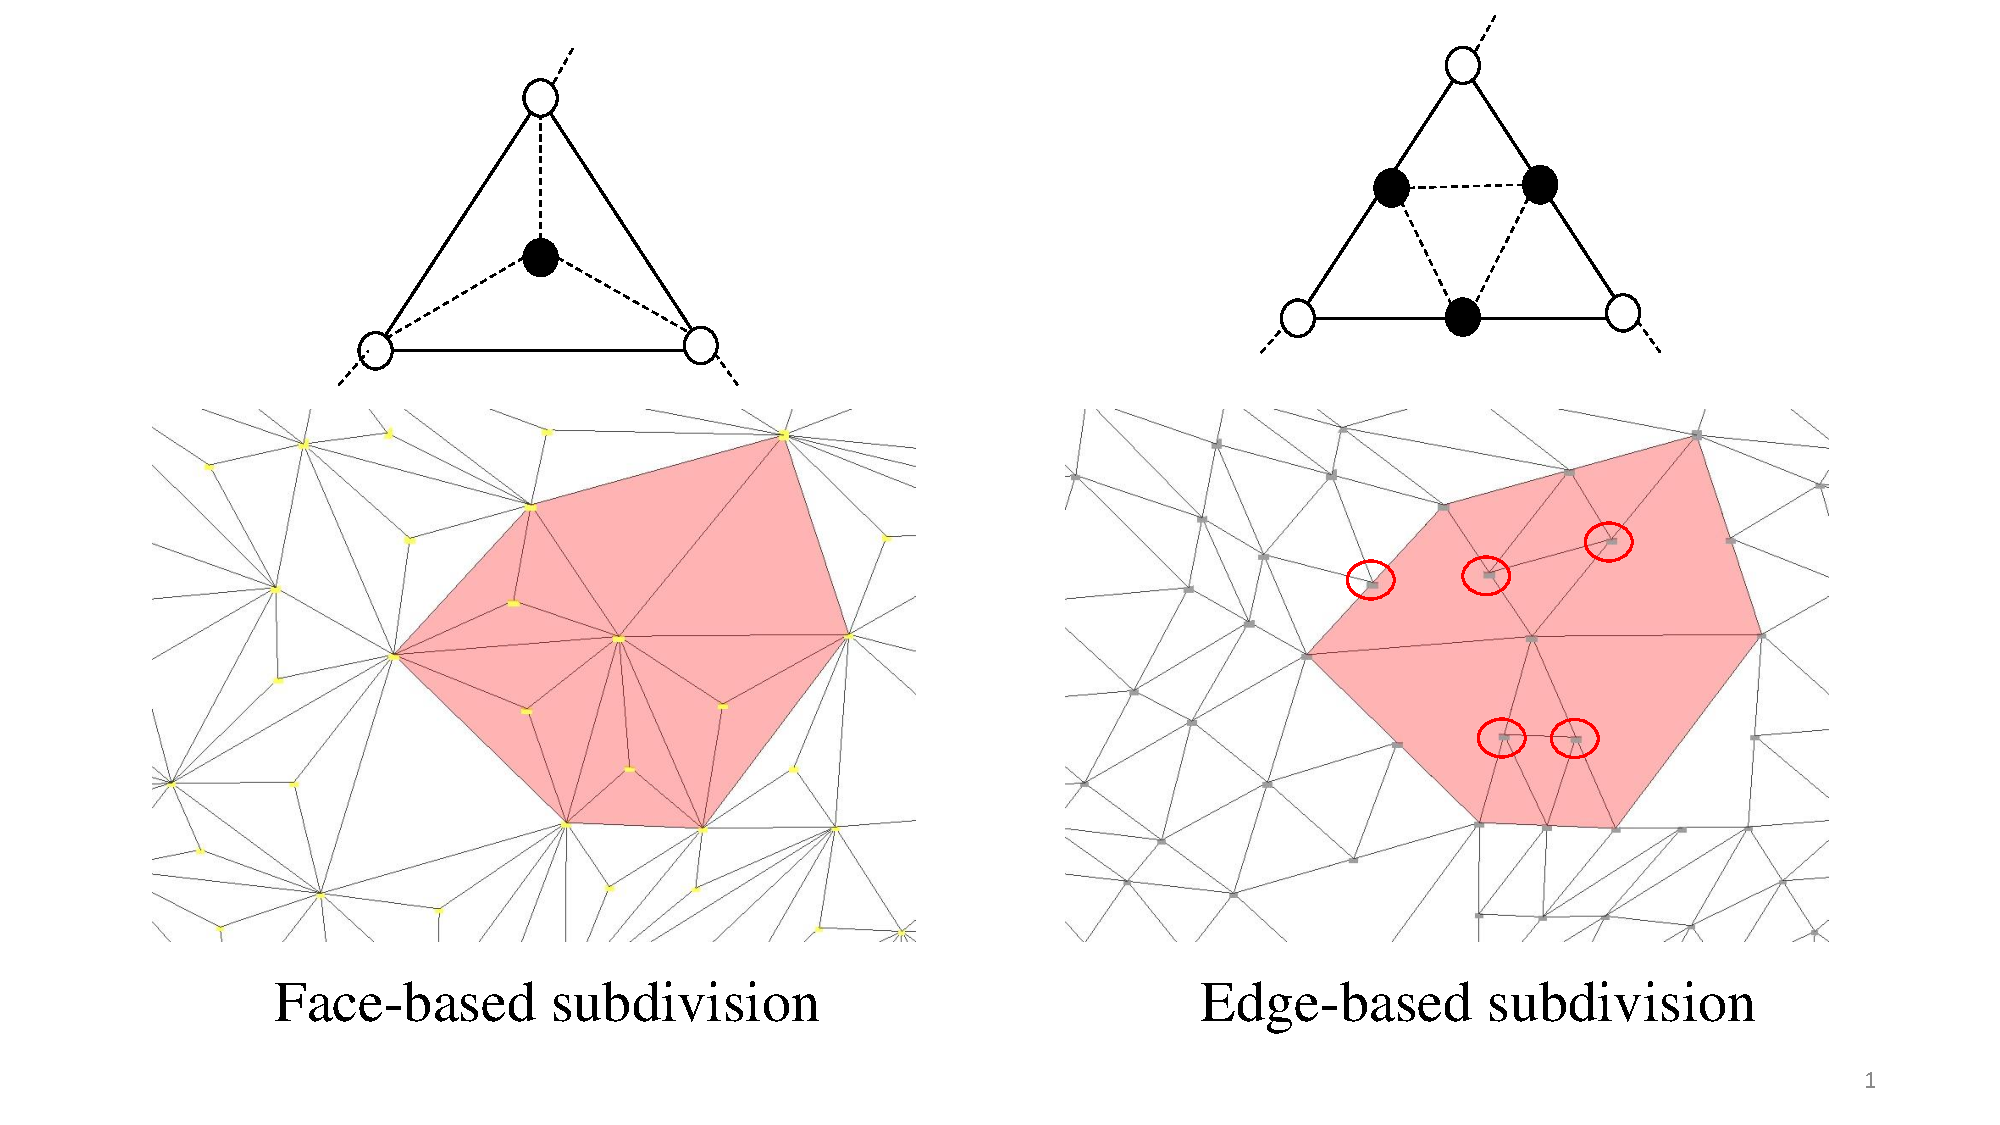
\includegraphics[width=1\linewidth]{pic/work2/Tri.pdf}
\bicaption{基于面和基于边的三角形细分方法的区别}{
Differences between face-based and edge-based triangle subdivision}
\label{fig:Triangles}
\end{figure}
\subsection{算法局限性}
本文采用联合优化方案能够解决三维模型重建误差较大的缺陷取得了一定的效果,但是经过研究发现仍然存在一定的不足。具体地,需要改进的地方如下:\par
\begin{enumerate}[label=(\arabic*),leftmargin=\parindent,align=left,labelwidth=\parindent,labelsep=0pt]
	\item 对于大场景下的纹理优化存在一定的局限性。在大场景下纹理图像需要多张并组合为完整的纹理场景,但是本文无法在优化多张纹理图时保证映射关系,所以本文只关注在单张纹理图可表达的场景。
	\item 无法估计场景光源。在室内点光源以及室外由于反射带来的高光会使被扫描物体表面产生亮点,遮盖了物体表面本身的色彩。优化结果会使物体的漫反射图和高光杂揉到一起无法分离,无法反映物体真实的纹理。 虽然本文能抵抗弱光源带来的误差,但是对于强光源带来的影响无法消除。
	\item 弱纹理场景优化效果不足。本文算法依赖于重投影误差,对于纹理简单的场景,该算法所带来的优化效果并不如纹理丰富的场景那么显著。具体地,无纹理或弱纹理区域,彩色图像上像素值差异不明显,需要利用深度图来协助监督。而且,当场景中弱纹理区域在平面上时,深度差异较小,会进一步减弱算法的监督效果。
\end{enumerate}

\section{本章小结}

本章提出了一种联合优化算法,用于优化RGB-D重建模型的纹理、相机和几何。该算法首先利用重投影误差矫正相机位姿,并应用变形场校正投影像素坐标;随后,利用一致的目标函数更新网格顶点位置,并采用自适应细分来增加网格高频几何细节;最后,本文采用对抗生成网络进行纹理图像重叠,并通过像素重生成管线使像素位置发生位移以抵消重建中的误差。经过联合优化,本文获得了高质量的几何模型、清晰的纹理图像以及精确的相机位姿。实验证明,本文的算法表现出了在各种不同场景下均能重建出高保真度纹理模型的优势。



% 第五章总结与展望
% !TeX root = ../Template.tex
% 总结


\summary

\section*{论文总结}


本文首先阐述了利用RGB-D相机进行三维重建与纹理优化的背景与意义,以及纹理优化领域的研究现状。然后,对纹理优化相关技术做了梳理与总结。针对目前纹理优化中纹理存在模糊伪影以及裂缝现象,本文提出基于深度学习的纹理优化方案,即利用可微分渲染技术矫正相机位姿,借助像素重生成管线重新生成新的纹理图像。为了保证在几何模型重建误差较大的情况下仍能获得高保真的纹理,本文进一步提出了基于可微分渲染的联合优化算法,它可以对初始估计的相机位姿、重建模型、纹理图集进行迭代优化,得到具有高频几何细节和清晰纹理贴图的模型。综上所述,本文贡献点有两个。\par
提出基于可微分渲染的相机位姿矫正与纹理合成算法,获得清晰纹理。首先利用渲染将初始纹理与三维模型渲染至目标视角,通过与真实图片做$L_1$损失,获得期望梯度以更新相机位姿。然后重新初始化纹理图并将纹理图设置为优化变量,利用对抗生成网络重合成清晰的纹理。经过纹理重合成,得到全局一致高保真纹理模型。\par
提出联合优化算法同时对RGB-D重建的相机位姿、几何细节和纹理细节进行联合优化,有效解决纹理重建过程中存在的几何、位姿误差以及各种噪声。在工作一基础上,本文利用可微分渲染优化三维模型顶点位置,对于三维模型中纹理丰富区域进行质心细分,以增加顶点和面片数目增强几何细节,引导顶点位置矫正。紧接着,本文提出交替优化策略分别对几何、纹理、位姿进行优化获取全局最优解。经过实验验证,本文提出的算法可以获得高保真的几何和纹理模型。
%==============================
\section*{未来展望}
由于在VR/AR、动画、视频游戏等领域有着广泛的应用前景,构建具有高保真纹理和几何图形的真实世界3D对象和场景一直是重要的问题。现阶段本文算法在纹理优化领域取得了一定的研究成果,但是还有很多问题需要进行解决。\par
目前,纹理优化领域所使用的数据集均由相关领域论文作者提供,缺乏第三方标准的公共数据集。由于拍摄场景、设备以及模型重建质量等因素的差异,评估纹理优化算法的效果面临一定的挑战。因此,下一步可以构建一些标准数据集,以供其他研究人员使用。这些数据集应该经过充分的策划和设计,以保证其中包含多样化的场景、设备和模型重建质量等。这样可以更加客观地评估纹理优化算法的表现,并促进该领域的发展。\par

当前的纹理优化算法主要以传统方法为主,与深度学习的结合还不够密切。对于基于数据驱动的算法,还存在一些缺陷。首先,这些算法更适合于小型场景的纹理优化,对于大型场景的表现不如传统算法。其次,在缺乏纹理或者仅具有单一颜色值的场景中,这些算法的纹理优化效果也会显著下降。未来的纹理优化算法需要具备更强的鲁棒性,并应当充分利用神经网络的学习能力,以对材质和灯光等因素进行建模,更加贴近真实世界的情况。\par
纹理依赖于几何模型存在,理论上几何模型重建越精确,纹理优化结果越好。不幸的是由于重建算法本身的缺陷或者物理遮挡使得几何模型会发生残缺现象。这破坏了几何模型的拓扑结构,为纹理优化带来新的挑战。未来可以先对几何模型缺失的地方进行补全,为后续获取高质量纹理模型提供保障。


%================= 参考文献(两种引用方法,建议第二种)==============================
% (一)用bib形式引入参考文献(某些参考文献有缺失)
% 2015版国标GBT7714-2015
% 2005版国标GBT7714-2005
% 用.bib文件形式引入参考文献
%\Bib{bst/GBT7714-2015}{ref}

%(二)手动添加参考文献(建议用这种),谷歌学术找国标格式的参考文献放入tex/References.tex中
\bib
\begin{thebibliography}{00}


\bibitem{RichardNewcombe2011KinectFusionRD} Newcombe R A, Izadi S, Hilliges O, et al. Kinectfusion: Real-time dense surface mapping and tracking[C].2011 10th IEEE international symposium on mixed and augmented reality. Ieee, 2011: 127-136.

\bibitem{ThomasWhelan2012KintinuousSE}
Whelan T, Kaess M, Fallon M, et al. Kintinuous: Spatially extended kinectfusion[J]. 2012.

\bibitem{ThomasWhelan2015ElasticFusionDS}Whelan T, Leutenegger S, Salas-Moreno R, et al. ElasticFusion: Dense SLAM without a pose graph[C]. Robotics: Science and Systems, 2015.


\bibitem{VictorAdrianPrisacariu2017InfiniTAMVA} Prisacariu V A, Kähler O, Golodetz S, et al. Infinitam v3: A framework for large-scale 3d reconstruction with loop closure[J]. arXiv preprint arXiv:1708.00783, 2017.

\bibitem{AngelaDai2016BundleFusionRG}Dai A, Nießner M, Zollhöfer M, et al. Bundlefusion: Real-time globally consistent 3d reconstruction using on-the-fly surface reintegration[J]. ACM Transactions on Graphics (ToG), 2017, 36(4): 1.

\bibitem{DejanAzinovic2021NeuralRS} Azinović D, Martin-Brualla R, Goldman D B, et al. Neural rgb-d surface reconstruction[C]. Proceedings of the IEEE/CVF Conference on Computer Vision and Pattern Recognition. 2022: 6290-6301.

\bibitem{fuyanping}付燕平.\enspace 面向RGB-D相机高保真三维重建与纹理映射研究[D]. \enspace 武汉大学,\enspace 2020. DOI:10.27379/d.cnki.gwhdu.2020.000647.
 
\bibitem{tongliyang}童立靖,\enspace 杨鑫坡.\enspace 基于相机标定的纹理映射方法[J].数字技术与应用,\enspace 2022,\enspace 40(09):1-3. DOI:10.19695/j.cnki.cn12-1369.2022.09.01.

\bibitem{maolibo}毛力波.\enspace 实景三维纹理映射与增强方法研究[D].\enspace 山东建筑大学, \! 2022. \enspace DOI:10.27273/d.cnki.gsajc.2022.000004.

\bibitem{lempitsky2007seamless}Lempitsky V, Ivanov D. Seamless mosaicing of image-based texture maps[C]. 2007 IEEE conference on computer vision and pattern recognition. IEEE, 2007: 1-6.


\bibitem{boykov2001fast}Boykov Y, Veksler O, Zabih R. Fast approximate energy minimization via graph cuts[J]. IEEE Transactions on pattern analysis and machine intelligence, 2001, 23(11): 1222-1239.

\bibitem{waechter2014let}Waechter M, Moehrle N, Goesele M. Let there be color! Large-scale texturing of 3D reconstructions[C]. Computer Vision–ECCV 2014: 13th European Conference, Zurich, Switzerland, September 6-12, 2014, Proceedings, Part V 13. Springer International Publishing, 2014: 836-850.


\bibitem{PrezPatrick2003PoissonIE}Pérez P, Gangnet M, Blake A. Poisson image editing[M]. ACM SIGGRAPH 2003 Papers. 2003: 313-318.

\bibitem{fu2018texture}Fu Y, Yan Q, Yang L, et al. Texture mapping for 3d reconstruction with rgb-d sensor[C]. Proceedings of the IEEE conference on computer vision and pattern recognition. 2018: 4645-4653.

\bibitem{franken2005minimizing}Franken T, Dellepiane M, Ganovelli F, et al. Minimizing user intervention in registering 2D images to 3D models[J]. The Visual Computer, 2005, 21: 619-628.

\bibitem{eisemann2008floating}Eisemann M, De Decker B, Magnor M, et al. Floating textures[C]. Computer graphics forum. Oxford, UK: Blackwell Publishing Ltd, 2008, 27(2): 409-418.

\bibitem{dellepiane2011flow}Dellepiane M, Marroquim R, Callieri M, et al. Flow-based local optimization for image-to-geometry projection[J]. IEEE Transactions on Visualization and Computer Graphics, 2011, 18(3): 463-474.

\bibitem{wu20083d}Wu C, Clipp B, Li X, et al. 3D model matching with viewpoint-invariant patches (VIP)[C]. 2008 IEEE Conference on Computer Vision and Pattern Recognition. IEEE, 2008: 1-8.

\bibitem{aganj2010multi}Aganj E, Monasse P, Keriven R. Multi-view texturing of imprecise mesh[C]. Computer Vision–ACCV 2009: 9th Asian Conference on Computer Vision, Xi’an, September 23-27, 2009, Revised Selected Papers, Part II 9. Springer Berlin Heidelberg, 2010: 468-476.

\bibitem{zhou2014color}Zhou Q Y, Koltun V. Color map optimization for 3d reconstruction with consumer depth cameras[J]. ACM Transactions on Graphics (ToG), 2014, 33(4): 1-10.

\bibitem{Barnes:2009:PAR}Barnes C, Shechtman E, Finkelstein A, et al. PatchMatch: A randomized correspondence algorithm for structural image editing[J]. ACM Trans. Graph., 2009, 28(3): 24.

\bibitem{bi2017patch}Bi S, Kalantari N K, Ramamoorthi R. Patch-based optimization for image-based texture mapping[J]. ACM Trans. Graph., 2017, 36(4): 106:1-106:11.

\bibitem{fu2021seamless}Fu Y, Yan Q, Liao J, et al. Seamless texture optimization for RGB-D reconstruction[J]. IEEE Transactions on Visualization and Computer Graphics, 2021.

\bibitem{RobertMaier2017Intrinsic3DH3}Maier R, Kim K, Cremers D, et al. Intrinsic3D: High-quality 3D reconstruction by joint appearance and geometry optimization with spatially-varying lighting[C]. Proceedings of the IEEE international conference on computer vision. 2017: 3114-3122. 

\bibitem{YanpingFu2020JointTA}Fu Y, Yan Q, Liao J, et al. Joint texture and geometry optimization for RGB-D reconstruction[C]. Proceedings of the IEEE/CVF Conference on Computer Vision and Pattern Recognition. 2020: 5950-5959.

\bibitem{NIPS2014_5ca3e9b1}Goodfellow I, Pouget-Abadie J, Mirza M, et al. Generative adversarial networks[J]. Communications of the ACM, 2020, 63(11): 139-144.

\bibitem{isola2017image}Isola P, Zhu J Y, Zhou T, et al. Image-to-image translation with conditional adversarial networks[C]. Proceedings of the IEEE conference on computer vision and pattern recognition. 2017: 1125-1134.

\bibitem{zhu2017unpaired}Zhu J Y, Park T, Isola P, et al. Unpaired image-to-image translation using cycle-consistent adversarial networks[C]. Proceedings of the IEEE international conference on computer vision. 2017: 2223-2232.

\bibitem{JingweiHuang2020AdversarialTO}Huang J, Thies J, Dai A, et al. Adversarial texture optimization from rgb-d scans[C]. Proceedings of the IEEE/CVF Conference on Computer Vision and Pattern Recognition. 2020: 1559-1568.


\bibitem{9705143}Zhang J, Wan Z, Liao J. Adaptive joint optimization for 3D reconstruction with differentiable rendering[J]. IEEE Transactions on Visualization and Computer Graphics, 2022.


\bibitem{chanmonteiro2020pi-GAN}Chan E R, Monteiro M, Kellnhofer P, et al. pi-gan: Periodic implicit generative adversarial networks for 3d-aware image synthesis[C]. Proceedings of the IEEE/CVF conference on computer vision and pattern recognition. 2021: 5799-5809.


\bibitem{888718}Zhang Z. A flexible new technique for camera calibration[J]. IEEE Transactions on pattern analysis and machine intelligence, 2000, 22(11): 1330-1334.

\bibitem{nguyen2018rendernet}Nguyen-Phuoc T H, Li C, Balaban S, et al. Rendernet: A deep convolutional network for differentiable rendering from 3d shapes[J]. Advances in neural information processing systems, 2018, 31.

\bibitem{BrianCurless1996AVM}Curless B, Levoy M. A volumetric method for building complex models from range images[C]. Proceedings of the 23rd annual conference on Computer graphics and interactive techniques. 1996: 303-312.

\bibitem{511}Levoy M. Display of surfaces from volume data[J]. IEEE Computer graphics and Applications, 1988, 8(3): 29-37.

\bibitem{lorensen1987marching}Lorensen W E, Cline H E. Marching cubes: A high resolution 3D surface construction algorithm[J]. ACM siggraph computer graphics, 1987, 21(4): 163-169.


\bibitem{LarsMescheder2018OccupancyNL}Mescheder L, Oechsle M, Niemeyer M, et al. Occupancy networks: Learning 3d reconstruction in function space[C]. Proceedings of the IEEE/CVF conference on computer vision and pattern recognition. 2019: 4460-4470.

\bibitem{mildenhall2021nerf}Mildenhall B, Srinivasan P P, Tancik M, et al. Nerf: Representing scenes as neural radiance fields for view synthesis[J]. Communications of the ACM, 2021, 65(1): 99-106.

\bibitem{park2019deepsdf}Park J J, Florence P, Straub J, et al. Deepsdf: Learning continuous signed distance functions for shape representation[C]. Proceedings of the IEEE/CVF conference on computer vision and pattern recognition. 2019: 165-174.

\bibitem{hart1996sphere}Hart J C. Sphere tracing: A geometric method for the antialiased ray tracing of implicit surfaces[J]. The Visual Computer, 1996, 12(10): 527-545.

\bibitem{Deepvoxels}Sitzmann V, Thies J, Heide F, et al. Deepvoxels: Learning persistent 3d feature embeddings[C]. Proceedings of the IEEE/CVF Conference on Computer Vision and Pattern Recognition. 2019: 2437-2446.

\bibitem{qi2017pointnet}Qi C R, Su H, Mo K, et al. Pointnet: Deep learning on point sets for 3d classification and segmentation[C]. Proceedings of the IEEE conference on computer vision and pattern recognition. 2017: 652-660.


\bibitem{qi2017pointnet++}Qi C R, Yi L, Su H, et al. Pointnet++: Deep hierarchical feature learning on point sets in a metric space[J]. Advances in neural information processing systems, 2017, 30.

\bibitem{kazhdan2006poisson}Kazhdan M, Bolitho M, Hoppe H. Poisson surface reconstruction[C]. Proceedings of the fourth Eurographics symposium on Geometry processing. 2006, 7: 0.

\bibitem {LocalChapterEvents:ItalChap:ItalianChapConf2008:129-136}Cignoni P, Callieri M, Corsini M, et al. Meshlab: an open-source mesh processing tool[C]. Eurographics Italian chapter conference. 2008, 2008: 129-136.

\bibitem{ShichenLiu2019SoftRA}Liu S, Li T, Chen W, et al. Soft rasterizer: A differentiable renderer for image-based 3d reasoning[C]. Proceedings of the IEEE/CVF International Conference on Computer Vision. 2019: 7708-7717.

\bibitem{shapenet2015}Chang A X, Funkhouser T, Guibas L, et al. Shapenet: An information-rich 3d model repository[J]. arXiv preprint arXiv:1512.03012, 2015.

\bibitem{greene1986environment}Greene N. Environment mapping and other applications of world projections[J]. IEEE computer graphics and Applications, 1986, 6(11): 21-29.

\bibitem{tarini2017rethinking} Tarini M, Yuksel C, Lefebvre S. Rethinking texture mapping[M]. ACM SIGGRAPH 2017 Courses. 2017: 1-139.

\bibitem{yuksel2019rethinking}Yuksel C, Lefebvre S, Tarini M. Rethinking texture mapping[C]. Computer Graphics Forum. 2019, 38(2): 535-551.

\bibitem{HiroharuKato2017Neural3M}Kato H, Ushiku Y, Harada T. Neural 3d mesh renderer[C]. Proceedings of the IEEE conference on computer vision and pattern recognition. 2018: 3907-3916.

\bibitem{yariv2020multiview}Yariv L, Kasten Y, Moran D, et al. Multiview neural surface reconstruction by disentangling geometry and appearance[J]. Advances in Neural Information Processing Systems, 2020, 33: 2492-2502.

\bibitem{zhang2020nerf++}Zhang K, Riegler G, Snavely N, et al. Nerf++: Analyzing and improving neural radiance fields[J]. arXiv preprint arXiv:2010.07492, 2020.

\bibitem{tewari2020state}Tewari A, Fried O, Thies J, et al. State of the art on neural rendering[C]. Computer Graphics Forum. 2020, 39(2): 701-727.


\bibitem{kajiya1986rendering}Kajiya J T. The rendering equation[C]. Proceedings of the 13th annual conference on Computer graphics and interactive techniques. 1986: 143-150.

\bibitem{blinn1977models}Blinn J F. Models of light reflection for computer synthesized pictures[C]. Proceedings of the 4th annual conference on Computer graphics and interactive techniques. 1977: 192-198.

\bibitem{niemeyer2020differentiable}Niemeyer M, Mescheder L, Oechsle M, et al. Differentiable volumetric rendering: Learning implicit 3d representations without 3d supervision[C]. Proceedings of the IEEE/CVF Conference on Computer Vision and Pattern Recognition. 2020: 3504-3515.

\bibitem{jiang2020sdfdiff}Jiang Y, Ji D, Han Z, et al. Sdfdiff: Differentiable rendering of signed distance fields for 3d shape optimization[C]. Proceedings of the IEEE/CVF Conference on Computer Vision and Pattern Recognition. 2020: 1251-1261.

\bibitem{liu2020dist}Liu S, Zhang Y, Peng S, et al. Dist: Rendering deep implicit signed distance function with differentiable sphere tracing[C]. Proceedings of the IEEE/CVF Conference on Computer Vision and Pattern Recognition. 2020: 2019-2028.

\bibitem{wiles2020synsin}Wiles O, Gkioxari G, Szeliski R, et al. Synsin: End-to-end view synthesis from a single image[C]. Proceedings of the IEEE/CVF Conference on Computer Vision and Pattern Recognition. 2020: 7467-7477.

\bibitem{lassner2021pulsar}Lassner C, Zollhofer M. Pulsar: Efficient sphere-based neural rendering[C]. Proceedings of the IEEE/CVF Conference on Computer Vision and Pattern Recognition. 2021: 1440-1449.

\bibitem{ravi2020pytorch3d}Ravi N, Reizenstein J, Novotny D, et al. Accelerating 3d deep learning with pytorch3d[J]. arXiv preprint arXiv:2007.08501, 2020.

\bibitem{SungjoonChoi2015RobustRO}Choi S, Zhou Q Y, Koltun V. Robust reconstruction of indoor scenes[C]. Proceedings of the IEEE Conference on Computer Vision and Pattern Recognition. 2015: 5556-5565.

 \bibitem{MatthiasNiener2013Realtime3R}Nießner M, Zollhöfer M, Izadi S, et al. Real-time 3D reconstruction at scale using voxel hashing[J]. ACM Transactions on Graphics (ToG), 2013, 32(6): 1-11.


\bibitem{sola2018micro}Sola J, Deray J, Atchuthan D. A micro Lie theory for state estimation in robotics[J]. arXiv preprint arXiv:1812.01537, 2018.


\bibitem{liu2020general}Liu S, Li T, Chen W, et al. A general differentiable mesh renderer for image-based 3D reasoning[J]. IEEE Transactions on Pattern Analysis and Machine Intelligence, 2020, 44(1): 50-62.

\bibitem{huang20173dlite}Huang J, Dai A, Guibas L J, et al. 3Dlite: towards commodity 3D scanning for content creation[J]. ACM Trans. Graph., 2017, 36(6): 203:1-203:14.

\bibitem{MatthewLoper2014OpenDRAA}Loper M M, Black M J. OpenDR: An approximate differentiable renderer[C]. Computer Vision–ECCV 2014: 13th European Conference, Zurich, Switzerland, September 6-12, 2014, Proceedings, Part VII 13. Springer International Publishing, 2014: 154-169.

\bibitem{niessner2013real}Nießner M, Zollhöfer M, Izadi S, et al. Real-time 3D reconstruction at scale using voxel hashing[J]. ACM Transactions on Graphics (ToG), 2013, 32(6): 1-11.

\bibitem{KyleGenova2018UnsupervisedTF}Genova K, Cole F, Maschinot A, et al. Unsupervised training for 3d morphable model regression[C]. Proceedings of the IEEE Conference on Computer Vision and Pattern Recognition. 2018: 8377-8386.

\bibitem{HelgeRhodin2015AVS}Rhodin H, Robertini N, Richardt C, et al. A versatile scene model with differentiable visibility applied to generative pose estimation[C]. Proceedings of the IEEE International Conference on Computer Vision. 2015: 765-773.

\bibitem{chen2019_dibr}Lyu H, Sha N, Qin S, et al. Advances in neural information processing systems[J]. Advances in neural information processing systems, 2019, 32.

\bibitem{fu2021auto}Fu L, Zhou C, Guo Q, et al. Auto-exposure fusion for single-image shadow removal[C]. Proceedings of the IEEE/CVF conference on computer vision and pattern recognition. 2021: 10571-10580.

\bibitem{fu2021multi}Fu G, Zhang Q, Zhu L, et al. A multi-task network for joint specular highlight detection and removal[C]. Proceedings of the IEEE/CVF Conference on Computer Vision and Pattern Recognition. 2021: 7752-7761.

\bibitem{sauer2023stylegan}Sauer A, Karras T, Laine S, et al. Stylegan-t: Unlocking the power of gans for fast large-scale text-to-image synthesis[J]. arXiv preprint arXiv:2301.09515, 2023.

\bibitem{yu2018generative}Yu J, Lin Z, Yang J, et al. Generative image inpainting with contextual attention[C]. Proceedings of the IEEE conference on computer vision and pattern recognition. 2018: 5505-5514.

\bibitem{wang2018high}Wang T C, Liu M Y, Zhu J Y, et al. High-resolution image synthesis and semantic manipulation with conditional gans[C]. Proceedings of the IEEE conference on computer vision and pattern recognition. 2018: 8798-8807.


\bibitem{LongYang2018SurfaceRV}Yang L, Yan Q, Fu Y, et al. Surface reconstruction via fusing sparse-sequence of depth images[J]. IEEE transactions on visualization and computer graphics, 2017, 24(2): 1190-1203.



\bibitem{FrederiqueCrete2007TheBE}Crete F, Dolmiere T, Ladret P, et al. The blur effect: perception and estimation with a new no-reference perceptual blur metric[C]. Human vision and electronic imaging XII. SPIE, 2007, 6492: 196-206.


\bibitem{besl1992method}Besl P J, McKay N D. Method for registration of 3-D shapes[C]. Sensor fusion IV: control paradigms and data structures. Spie, 1992, 1611: 586-606.


\bibitem{chen1992object}Chen Y, Medioni G. Object modelling by registration of multiple range images[J]. Image and vision computing, 1992, 10(3): 145-155.

\bibitem{wedderburn1974quasi}Wedderburn R W M. Quasi-likelihood functions, generalized linear models, and the Gauss—Newton method[J]. Biometrika, 1974, 61(3): 439-447.


\bibitem{liu2018intriguing}Liu R, Lehman J, Molino P, et al. An intriguing failing of convolutional neural networks and the coordconv solution[J]. Advances in neural information processing systems, 2018, 31.

\bibitem{de2003improved}De Boer J F, Cense B, Park B H, et al. Improved signal-to-noise ratio in spectral-domain compared with time-domain optical coherence tomography[J]. Optics letters, 2003, 28(21): 2067-2069.

\bibitem{brunet2011mathematical}Brunet D, Vrscay E R, Wang Z. On the mathematical properties of the structural similarity index[J]. IEEE Transactions on Image Processing, 2011, 21(4): 1488-1499.

\bibitem{zhang2018unreasonable}Zhang R, Isola P, Efros A A, et al. The unreasonable effectiveness of deep features as a perceptual metric[C]. Proceedings of the IEEE conference on computer vision and pattern recognition. 2018: 586-595.

\bibitem{kingma2014adam}Kingma D P, Ba J. Adam: A method for stochastic optimization[J]. arXiv preprint arXiv:1412.6980, 2014.

\bibitem{newcombe2015dynamicfusion} Newcombe R A, Fox D, Seitz S M. Dynamicfusion: Reconstruction and tracking of non-rigid scenes in real-time[C]. Proceedings of the IEEE conference on computer vision and pattern recognition. 2015: 343-352.

\bibitem{innmann2016volumedeform} Innmann M, Zollhöfer M, Nießner M, et al. Volumedeform: Real-time volumetric non-rigid reconstruction[C]. Computer Vision–ECCV 2016: 14th European Conference, Amsterdam, The Netherlands, October 11-14, 2016, Proceedings, Part VIII 14. Springer International Publishing, 2016: 362-379.

\bibitem{yu2017bodyfusion}Yu T, Guo K, Xu F, et al. Bodyfusion: Real-time capture of human motion and surface geometry using a single depth camera[C]. Proceedings of the IEEE International Conference on Computer Vision. 2017: 910-919.

\bibitem{yu2018doublefusion}Yu T, Zheng Z, Guo K, et al. Doublefusion: Real-time capture of human performances with inner body shapes from a single depth sensor[C]. Proceedings of the IEEE conference on computer vision and pattern recognition. 2018: 7287-7296.

\bibitem{xu2019unstructuredfusion}Xu L, Su Z, Han L, et al. Unstructuredfusion: realtime 4d geometry and texture reconstruction using commercial rgbd cameras[J]. IEEE transactions on pattern analysis and machine intelligence, 2019, 42(10): 2508-2522.

\bibitem{su2020robustfusion} Su Z, Xu L, Zheng Z, et al. Robustfusion: Human volumetric capture with data-driven visual cues using a rgbd camera[C]. Computer Vision–ECCV 2020: 16th European Conference, Glasgow, UK, August 23–28, 2020, Proceedings, Part IV 16. Springer International Publishing, 2020: 246-264.


\bibitem{slavcheva2017killingfusion}Slavcheva M, Baust M, Cremers D, et al. Killingfusion: Non-rigid 3d reconstruction without correspondences[C]. Proceedings of the IEEE Conference on Computer Vision and Pattern Recognition. 2017: 1386-1395.

\bibitem{gao2019surfelwarp}Gao W, Tedrake R. Surfelwarp: Efficient non-volumetric single view dynamic reconstruction[J]. arXiv preprint arXiv:1904.13073, 2019.

\bibitem{dou2016fusion4d}Dou M, Khamis S, Degtyarev Y, et al. Fusion4d: Real-time performance capture of challenging scenes[J]. ACM Transactions on Graphics (ToG), 2016, 35(4): 1-13.

\bibitem{ChengleiWu2014RealtimeSR}Wu C, Zollhöfer M, Nießner M, et al. Real-time shading-based refinement for consumer depth cameras[J]. ACM Transactions on Graphics (ToG), 2014, 33(6): 1-10.

\bibitem{HiroharuKato2020DifferentiableRA}Kato H, Beker D, Morariu M, et al. Differentiable rendering: A survey[J]. arXiv preprint arXiv:2006.12057, 2020.

\bibitem{agarap2018deep}Agarap A F. Deep learning using rectified linear units (relu)[J]. arXiv preprint arXiv:1803.08375, 2018.

\bibitem{jiang2021focal}Jiang L, Dai B, Wu W, et al. Focal frequency loss for image reconstruction and synthesis[C]. Proceedings of the IEEE/CVF International Conference on Computer Vision. 2021: 13919-13929.
\bibitem{Zhou2018}Zhou Q Y, Park J, Koltun V. Open3D: A modern library for 3D data processing[J]. arXiv preprint arXiv:1801.09847, 2018.





%------------------------------------------未引用--------------------------
% \bibitem{dosovitskiy2016generating}Dosovitskiy A, Brox T. Generating images with perceptual similarity metrics based on deep networks[J]. Advances in neural information processing systems, 2016, 29.
% \bibitem{dessein2014seamless}Dessein A, Smith W A P, Wilson R C, et al. Seamless texture stitching on a 3D mesh by poisson blending in patches[C]. 2014 IEEE International Conference on Image Processing (ICIP). IEEE, 2014: 2031-2035.
% \bibitem{johnson2016perceptual}Johnson J, Alahi A, Fei-Fei L. Perceptual losses for real-time style transfer and super-resolution[C]. Computer Vision–ECCV 2016: 14th European Conference, Amsterdam, The Netherlands, October 11-14, 2016, Proceedings, Part II 14. Springer International Publishing, 2016: 694-711.
% \bibitem{karras2017progressive}Karras T, Aila T, Laine S, et al. Progressive growing of gans for improved quality, stability, and variation[J]. arXiv preprint arXiv:1710.10196, 2017.
% \bibitem{vu2011bf}Vu C T, Phan T D, Chandler D M. ${\bf S} _ {3} $: a spectral and spatial measure of local perceived sharpness in natural images[J]. IEEE transactions on image processing, 2011, 21(3): 934-945.
% \bibitem{simakov2008summarizing}Simakov D, Caspi Y, Shechtman E, et al. Summarizing visual data using bidirectional similarity[C]. 2008 IEEE Conference on Computer Vision and Pattern Recognition. IEEE, 2008: 1-8.
% \bibitem{KaolinLibrary}Jatavallabhula K M, Smith E, Lafleche J F, et al. Kaolin: A pytorch library for accelerating 3d deep learning research[J]. arXiv preprint arXiv:1911.05063, 2019.
% \bibitem{fuyanping}[1]付燕平. 面向RGB-D相机高保真三维重建与纹理映射研究[D].武汉大学,2020.DOI:10.27379/d.cnki.gwhdu.2020.000647.
% \bibitem{tongliyang}[1]童立靖,杨鑫坡.基于相机标定的纹理映射方法[J].数字技术与应用,2022,40(09):1-3.DOI:10.19695/j.cnki.cn12-1369.2022.09.01.

% \bibitem{maolibo}[1]毛力波. 实景三维纹理映射与增强方法研究[D].山东建筑大学,2022.DOI:10.27273/d.cnki.gsajc.2022.000004.


\end{thebibliography}

% 附录,暂时用不到
% % !TeX root = ../Template.tex
% [附录]
\appendix

下列内容可以作为附录:

\begin{enumerate}[label=\arabic*)]
\item 为了整篇论文材料的完整,但编入正文又有损于编排的条理和逻辑性,这一材料包括比正文更为详尽的信息、研究方法和技术更深入的叙述,建议可以阅读的参考文献题录,对了解正文内容有用的补充信息等;
\item 由于篇幅过大或取材于复制品而不便于编入正文的材料;
\item 不便于编入正文的罕见的珍贵或需要特别保密的技术细节和详细方案(这中情况可单列成册);
\item 对一般读者并非必要阅读,但对专业同行有参考价值的资料;
\item 某些重要的原始数据、过长的数学推导、计算程序、框图、结构图、注释、统计表、计算机打印输出文件等。
\end{enumerate}

\par * 嗯,自由发挥吧 * \par

% 攻读学位期间成果
% !TeX root = ../Template.tex
% [攻读学位期间取得的成果]
% \clearemptydoublepage

\achievement

\begin{enumerate}[leftmargin =0.7cm]
\renewcommand{\labelenumi}{[\theenumi]}
\item  一种基于几何先验与shading线索的三维重建方法(专利,初审合格)
% \item Neural Reconstruction of Indoor Scenes using Geometric and Shading Cues(论文,在审)
\item 本人第一作者、导师通讯作者。 3D Reconstruction and Texture Optimization Based on Differentiable Rendering[C]. In 2023 8th International Conference on Intelligent Computing and Signal Processing (ICSP 2023)(已录用)

\end{enumerate}



% 攻读学位参与的科研项目
% !TeX root = ../Template.tex
% [攻读学位期间参与的科研项目]
% \clearemptydoublepage

\program


% (1)安徽省教育厅,安徽高校协同创新,GXXT-2022-029,基于三维视觉的MRI头动实时定量监测和MRI图像重建,2022-07 至 2024-07,100万元,在研,主持
\noindent[1] CCF-腾讯犀牛鸟科研基金,技术开发,CCF-Tencent RAGR20210117,面向移动终端基于RGB-D 相机的人体三维重建与纹理优化,2021-10 至 2022-10,15万元,本人在研,导师主持

% 致谢,在盲审模式下需要注释掉。
% !TeX root = ../Template.tex
% [致谢]
% \clearemptydoublepage

\acknowledgments

% 在我的硕士研究期间,我得到了很多人的支持和帮助。在此,我想向他们表达我的真挚感谢和敬意。\par

% 首先,我要感谢我的导师付燕平和赵海峰老师。他们是我研究工作的指导者和启蒙者。他们在我的研究过程中给予了我很多的指导和建议,让我不断成长和进步。他们的热情和专业精神激励着我,让我有了更深刻的认识和更广阔的眼界。他们的严谨治学精神、卓越学术水平、和渊博的学识都让我受益匪浅。在此,我向他们表达我最崇高的敬意和感谢之情。

% 其次,我要感谢我的同学们。他们是我研究过程中的知音和朋友。我们在实验室里一起讨论问题,分享研究成果,交流心得体会。他们的智慧和思考方式对我的研究有着很大的帮助。我也很感激他们对我的鼓励和支持,让我能够一路走来。

% 此外,我还要感谢我的朋友们。他们在我研究过程中给予了我很多的支持和帮助。他们在我最困难的时候给予我精神上的支持和鼓励,帮助我克服了许多困难。
% 我还要感谢我的家人。他们是我坚实的后盾和支持者。在我研究过程中,他们给予了我无微不至的关爱和支持。他们为我排忧解难,鼓励我不断前行,让我能够全心全意地投入研究工作,无后顾之忧。我感激他们一直以来的鼓励和支持,让我成为了一个更加自信和坚强的人。他们的支持和鼓励是我前进的动力源泉。

% 总之,我要再次感谢所有支持和帮助我的人。在这个过程中,我得到了很多的启示和启发,学到了很多的知识和技能。我也学会了如何独立思考和解决问题。这些经验和知识将对我今后的学习和工作产生重要的影响和指导。再次感谢大家,祝愿大家在未来的学习和工作中,取得更大的成就和进步!
% \par 


在我完成硕士研究的这段时间里,我受到了许多人的支持和帮助。在此,我想向所有给予我支持和鼓励的人表示最衷心的感谢和敬意。

首先,我要衷心感谢我的导师付燕平和赵海峰老师。他们是我研究工作的指导者和启蒙者,他们对我学术上的悉心指导和研究思路的启发使我受益匪浅。付燕平老师的严谨治学精神和卓越学术水平,赵海峰老师的渊博知识和学术见解,都深深地影响和激励着我。他们的耐心指导和不断鼓励让我能够顺利完成研究工作。在此,我向付燕平和赵海峰老师表达我最崇高的敬意和由衷的感谢。
我要特别感谢我的师兄聂和兵(博士),你对我的悉心指导和无私帮助让我受益匪浅。你的经验和见解对我的研究起到了重要的推动作用。
我还要感谢我的同门陈俏俏、盖振宇、韩润杰、邵愉快、刘晨、刘金宇、颜坤、晁胜阳、陈泉满、万宏志、刘浩。在这段时间里,我们一起度过了许多宝贵的时光。你们的智慧和思考方式一直是我学习的榜样,我们共同探讨问题、交流经验,互相鼓励和支持。你们的友谊和合作使得我的研究之旅更加丰富多彩。
特别感谢我的师弟们周锐、闫奇和王子阳等人,你们的努力和进步给我留下了深刻的印象。希望你们在未来的学术道路上不断努力,取得更好的成绩。我要特别感谢我的师妹江海燕,平时对我的鼓励使我受益匪浅。你的聪明才智和勤奋努力是我们大家的榜样,衷心感谢你的支持,祝你以后取得更好的成就。我还要感谢我的室友们章岩松、杨超和王锦涛。你们在生活中的陪伴和支持让我感到温暖和快乐。在你们的陪伴下,我能够更好地投入到研究工作中。

最后,我要感谢我的家人。你们是我坚实的后盾和永远的支持者。在我整个研究过程中,你们给予了我无微不至
的关怀和支持。无论是物质上的帮助还是精神上的鼓励,都让我感到无比幸福和感激。你们对我的包容和理解使我能够专注于研究,无后顾之忧。我感激你们一直以来的鼓励和支持,你们是我前进的动力源泉。

在这个研究过程中,我得到了很多宝贵的启示和经验,学到了许多知识和技能。这些将对我未来的学习和工作产生重要的影响和指导。我也学会了独立思考和解决问题的能力,这些都离不开各位的支持和帮助。再次向所有给予我支持和帮助的人表示最真挚的感谢。愿你们在未来的学习和工作中取得更大的成就和进步!







% 作者简介,暂时用不到
%% !TeX root = ../Template.tex
% [作者简介]
\biography
博士学位论文应该提供作者简介,主要包括:姓名、性别、出生年月日、民族、出生的;简要学历、工作经历(职务);以及攻读博士学位期间获得的其他奖项(除攻读学位期间取得的研究成果之外)。

\par * 嗯,“硕士学位论文无此项”,《手册》上是这么说的 * \par

\end{document} 

%-======================================================
% %添加空白页面命令
% \myemptypage